% Options for packages loaded elsewhere
\PassOptionsToPackage{unicode}{hyperref}
\PassOptionsToPackage{hyphens}{url}
%
\documentclass[
]{book}
\usepackage{amsmath,amssymb}
\usepackage{lmodern}
\usepackage{iftex}
\ifPDFTeX
  \usepackage[T1]{fontenc}
  \usepackage[utf8]{inputenc}
  \usepackage{textcomp} % provide euro and other symbols
\else % if luatex or xetex
  \usepackage{unicode-math}
  \defaultfontfeatures{Scale=MatchLowercase}
  \defaultfontfeatures[\rmfamily]{Ligatures=TeX,Scale=1}
\fi
% Use upquote if available, for straight quotes in verbatim environments
\IfFileExists{upquote.sty}{\usepackage{upquote}}{}
\IfFileExists{microtype.sty}{% use microtype if available
  \usepackage[]{microtype}
  \UseMicrotypeSet[protrusion]{basicmath} % disable protrusion for tt fonts
}{}
\makeatletter
\@ifundefined{KOMAClassName}{% if non-KOMA class
  \IfFileExists{parskip.sty}{%
    \usepackage{parskip}
  }{% else
    \setlength{\parindent}{0pt}
    \setlength{\parskip}{6pt plus 2pt minus 1pt}}
}{% if KOMA class
  \KOMAoptions{parskip=half}}
\makeatother
\usepackage{xcolor}
\usepackage{color}
\usepackage{fancyvrb}
\newcommand{\VerbBar}{|}
\newcommand{\VERB}{\Verb[commandchars=\\\{\}]}
\DefineVerbatimEnvironment{Highlighting}{Verbatim}{commandchars=\\\{\}}
% Add ',fontsize=\small' for more characters per line
\usepackage{framed}
\definecolor{shadecolor}{RGB}{248,248,248}
\newenvironment{Shaded}{\begin{snugshade}}{\end{snugshade}}
\newcommand{\AlertTok}[1]{\textcolor[rgb]{0.94,0.16,0.16}{#1}}
\newcommand{\AnnotationTok}[1]{\textcolor[rgb]{0.56,0.35,0.01}{\textbf{\textit{#1}}}}
\newcommand{\AttributeTok}[1]{\textcolor[rgb]{0.77,0.63,0.00}{#1}}
\newcommand{\BaseNTok}[1]{\textcolor[rgb]{0.00,0.00,0.81}{#1}}
\newcommand{\BuiltInTok}[1]{#1}
\newcommand{\CharTok}[1]{\textcolor[rgb]{0.31,0.60,0.02}{#1}}
\newcommand{\CommentTok}[1]{\textcolor[rgb]{0.56,0.35,0.01}{\textit{#1}}}
\newcommand{\CommentVarTok}[1]{\textcolor[rgb]{0.56,0.35,0.01}{\textbf{\textit{#1}}}}
\newcommand{\ConstantTok}[1]{\textcolor[rgb]{0.00,0.00,0.00}{#1}}
\newcommand{\ControlFlowTok}[1]{\textcolor[rgb]{0.13,0.29,0.53}{\textbf{#1}}}
\newcommand{\DataTypeTok}[1]{\textcolor[rgb]{0.13,0.29,0.53}{#1}}
\newcommand{\DecValTok}[1]{\textcolor[rgb]{0.00,0.00,0.81}{#1}}
\newcommand{\DocumentationTok}[1]{\textcolor[rgb]{0.56,0.35,0.01}{\textbf{\textit{#1}}}}
\newcommand{\ErrorTok}[1]{\textcolor[rgb]{0.64,0.00,0.00}{\textbf{#1}}}
\newcommand{\ExtensionTok}[1]{#1}
\newcommand{\FloatTok}[1]{\textcolor[rgb]{0.00,0.00,0.81}{#1}}
\newcommand{\FunctionTok}[1]{\textcolor[rgb]{0.00,0.00,0.00}{#1}}
\newcommand{\ImportTok}[1]{#1}
\newcommand{\InformationTok}[1]{\textcolor[rgb]{0.56,0.35,0.01}{\textbf{\textit{#1}}}}
\newcommand{\KeywordTok}[1]{\textcolor[rgb]{0.13,0.29,0.53}{\textbf{#1}}}
\newcommand{\NormalTok}[1]{#1}
\newcommand{\OperatorTok}[1]{\textcolor[rgb]{0.81,0.36,0.00}{\textbf{#1}}}
\newcommand{\OtherTok}[1]{\textcolor[rgb]{0.56,0.35,0.01}{#1}}
\newcommand{\PreprocessorTok}[1]{\textcolor[rgb]{0.56,0.35,0.01}{\textit{#1}}}
\newcommand{\RegionMarkerTok}[1]{#1}
\newcommand{\SpecialCharTok}[1]{\textcolor[rgb]{0.00,0.00,0.00}{#1}}
\newcommand{\SpecialStringTok}[1]{\textcolor[rgb]{0.31,0.60,0.02}{#1}}
\newcommand{\StringTok}[1]{\textcolor[rgb]{0.31,0.60,0.02}{#1}}
\newcommand{\VariableTok}[1]{\textcolor[rgb]{0.00,0.00,0.00}{#1}}
\newcommand{\VerbatimStringTok}[1]{\textcolor[rgb]{0.31,0.60,0.02}{#1}}
\newcommand{\WarningTok}[1]{\textcolor[rgb]{0.56,0.35,0.01}{\textbf{\textit{#1}}}}
\usepackage{longtable,booktabs,array}
\usepackage{calc} % for calculating minipage widths
% Correct order of tables after \paragraph or \subparagraph
\usepackage{etoolbox}
\makeatletter
\patchcmd\longtable{\par}{\if@noskipsec\mbox{}\fi\par}{}{}
\makeatother
% Allow footnotes in longtable head/foot
\IfFileExists{footnotehyper.sty}{\usepackage{footnotehyper}}{\usepackage{footnote}}
\makesavenoteenv{longtable}
\usepackage{graphicx}
\makeatletter
\def\maxwidth{\ifdim\Gin@nat@width>\linewidth\linewidth\else\Gin@nat@width\fi}
\def\maxheight{\ifdim\Gin@nat@height>\textheight\textheight\else\Gin@nat@height\fi}
\makeatother
% Scale images if necessary, so that they will not overflow the page
% margins by default, and it is still possible to overwrite the defaults
% using explicit options in \includegraphics[width, height, ...]{}
\setkeys{Gin}{width=\maxwidth,height=\maxheight,keepaspectratio}
% Set default figure placement to htbp
\makeatletter
\def\fps@figure{htbp}
\makeatother
\setlength{\emergencystretch}{3em} % prevent overfull lines
\providecommand{\tightlist}{%
  \setlength{\itemsep}{0pt}\setlength{\parskip}{0pt}}
\setcounter{secnumdepth}{5}
\usepackage{booktabs}
\ifLuaTeX
  \usepackage{selnolig}  % disable illegal ligatures
\fi
\usepackage[]{natbib}
\bibliographystyle{plainnat}
\IfFileExists{bookmark.sty}{\usepackage{bookmark}}{\usepackage{hyperref}}
\IfFileExists{xurl.sty}{\usepackage{xurl}}{} % add URL line breaks if available
\urlstyle{same} % disable monospaced font for URLs
\hypersetup{
  pdftitle={r4Casal2},
  pdfauthor={C. Marsh \& A. Dunn},
  hidelinks,
  pdfcreator={LaTeX via pandoc}}

\title{r4Casal2}
\author{C. Marsh \& A. Dunn}
\date{2023-06-22}

\begin{document}
\maketitle

{
\setcounter{tocdepth}{1}
\tableofcontents
}
\hypertarget{welcolme-to-r4casal2}{%
\chapter{\texorpdfstring{Welcolme to \textbf{r4Casal2}}{Welcolme to r4Casal2}}\label{welcolme-to-r4casal2}}

This book demonstrates functionality of the \texttt{r4Casal2} R package. This is an R package that works with the \texttt{Casal2} base R-library \href{https://github.com/alistairdunn1/CASAL2/tree/master/R-libraries}{found here}, although it is advised to use the R-library that is included with the Casal2 binary and usermanual you acquired. The \texttt{Casal2} base R-library is responsible for reading in output and interacting with Casal2 configuration files. The \texttt{r4Casal2} R package has been built for summarising and visualising objects read in from the base \texttt{Casal2} R-library.

This repository is a clone of Casal2 of \url{https://github.com/NIWAFisheriesModelling/r4Casal2}. It is intended to have additional bug fixes and enhancements for potential inclusion into the original NIWA codebase.

All functions in this package should be documented using the \texttt{roxygen} syntax with input parameters available using the \texttt{?} query. For example \texttt{?get\_fisheries}. To get a list of functions and general info on the package you can use \texttt{library(help="r4Casal2")} or see Section \ref{functionlist} for another list

\begin{Shaded}
\begin{Highlighting}[]
\FunctionTok{library}\NormalTok{(r4Casal2)}
\FunctionTok{library}\NormalTok{(Casal2)}
\FunctionTok{library}\NormalTok{(knitr)}
\FunctionTok{library}\NormalTok{(ggplot2)}
\FunctionTok{library}\NormalTok{(dplyr)}
\FunctionTok{library}\NormalTok{(reshape2)}
\FunctionTok{library}\NormalTok{(tidyr)}
\end{Highlighting}
\end{Shaded}

The core functionality of \texttt{r4Casal2} are its accessor functions. These are functions that will return a specific object from a range of Casal2 objects in long format that are \texttt{ggplot}, \texttt{dplyr} friendly. Most accessors start with \texttt{get\_} and should be self explanatory. There are some plotting functions, but I have found that I often want to custom ggplots and so mainly have custom plots. The accessors are coded to deal with three types of outpus. These are;

\begin{itemize}
\tightlist
\item
  \texttt{extract.mpd()} where Casal2 has been run with default report style. These objects are of class \texttt{casal2MPD} which are set by the Casal2 base function
\item
  \texttt{extract.mpd()} where Casal2 has been run with tabular reports \texttt{casal2\ -\/-tabular} or \texttt{casal2\ -t}. These objects are of class \texttt{casal2TAB} which are set by the Casal2 base function
\item
  \texttt{list} this is a list of \texttt{casal2MPD} which is a useful format for comparing MPD runs see Section \ref{summarisemultipleinputs}
\end{itemize}

\hypertarget{functionlist}{%
\chapter{\texorpdfstring{A list of key functions in the \texttt{r4Casal2} package}{A list of key functions in the r4Casal2 package}}\label{functionlist}}

\hypertarget{accessor-functions}{%
\section{Accessor functions}\label{accessor-functions}}

\begin{itemize}
\item
  \texttt{get\_derived\_quantities()} (or in shorthand form \texttt{get\_dqs()}). These will return all the derived quantities for a model output.
\item
  \texttt{get\_selectivities} will return a data frame with all the selectivity reports for a model output.
\item
  \texttt{get\_selectivities\_by\_year} will return a data frame with all the reports of type \texttt{selectivity\_by\_year} from a model output.
\item
  \texttt{get\_catchabilities} will return a data frame with all the catchability reports for a model output.
\item
  \texttt{get\_fisheries} will return a data frame with information from an \texttt{instantaneous\_mortality} process for a model output.
\item
  \texttt{get\_BH\_recruitment} will return a data frame with information from a \texttt{recruitment\_beverton\_holt} process for a model output.
\item
  \texttt{get\_abundance\_observations} will return a data frame with information from an \texttt{abundance} or \texttt{biomass} observation for a model output.
\item
  \texttt{get\_composition\_observations} will return a data frame with information from an \texttt{proportion\_at\_length}, \texttt{proportion\_at\_age}, \texttt{process\_removals\_by\_age} and \texttt{process\_removals\_by\_length} observation for a model output.
\item
  \texttt{get\_composition\_mean\_bin} will return a data frame with information from an \texttt{proportion\_at\_length}, \texttt{proportion\_at\_age}, \texttt{process\_removals\_by\_age} and \texttt{process\_removals\_by\_length} summarised as the mean length or mean age.
\item
  \texttt{get\_tag\_recapture\_observations} will return a data frame with information from an \texttt{tag\_recapture\_by\_length\_for\_growth}, \texttt{tag\_recapture\_by\_length} and \texttt{tag\_recapture\_by\_age} observation for a model output.
\item
  \texttt{get\_partition} will return a data frame with partition data from \texttt{partition} report.
\item
  \texttt{get\_initial\_partition} will return a data frame with initial partition \texttt{initialisation\_partition} report.
\item
  \texttt{get\_profile} Will return a data frame for a \texttt{profile} report.
\item
  \texttt{get\_estimated\_values} Will return a data frame for a \texttt{estimate\_value} report.
\item
  \texttt{get\_transformed\_parameters} Will return a data frame for a \texttt{parameter\_transformations} report.
\item
  \texttt{get\_timevarying\_parameters} Will return a data frame for a \texttt{time\_varying} report.
\item
  \texttt{get\_simulated\_age\_resids} Will reformat simulated data read in by the \texttt{read.simulated.data} function.
\item
  \texttt{get\_projections} will return a data frame of all \texttt{projection} reports from a model output.
\item
  \texttt{get\_growth} will return a data frame of all \texttt{age\_length} report from a model output.
\item
  \texttt{get\_covariance} will return a data frame of all \texttt{covariance\_matrix} report from a model output.
\end{itemize}

\hypertarget{other-useful-functions}{%
\section{Other useful functions}\label{other-useful-functions}}

\begin{itemize}
\item
  \texttt{aggregate\_objective\_report} This reformats an objective function report to be ``similar'' to CASALs output.
\item
  \texttt{create\_simulation\_reports} This will create a range of \texttt{@report.type=simulated\_observation} Casal2 reports that can help set up simulations. See Section \ref{PPC} on why you want to do this.
\item
  \texttt{build\_assessment\_bookdown} This will create a bookdown template for an assessment model MPD run.
\item
  \texttt{summarise\_config} Will summarize input files see Section \ref{summariseinputs}
\item
  \texttt{calculate\_composition\_stage\_two\_weights} Calculates the stage-two weights using \citet{francis2011data} TA1.8 method.
\item
  \texttt{get\_high\_correlations} Returns index of parameters that have high correlations from MPD. This requires the Casal2 model to have reported the \texttt{correlation\_matrix}
\item
  \texttt{run\_automatic\_reweighting} Automatically apply iterative reweighting methods for a Casal2 model
\item
  \texttt{extract\_reweighted\_mpds} extract all the reweighted mpds that are created by \texttt{run\_automatic\_reweighting}. Useful to then plot the effect of reweighting
\item
  \texttt{error\_value\_table} Create a data.frame of all observations from a casal2 mpd run outlining likelihood type, observation type and error value by year and observation.
\item
  \texttt{summarise\_estimated\_parameters} If a model reports \texttt{estimate\_summary} this function will extract two data frames that can be used to assess starting values and estimated values along with prior assumptions.
\item
  \texttt{plot\_profile} Will plot profiles for reports that have been run with \texttt{casal2\ -p} format.
\end{itemize}

\hypertarget{summariseinputs}{%
\chapter{Summarise configuration inputs}\label{summariseinputs}}

The \texttt{r4Casal2} has some functions that summarise a set of input files and returns a summary of the key model attributes. It can be difficult to know all the working parts in a Casal2 model. This is compounded when users make tweaks during an assessment and so the initial assumptions will not correspond to the final assumptions. The key function is \texttt{summarise\_config}

\hypertarget{example-files}{%
\section{Example files}\label{example-files}}

\begin{Shaded}
\begin{Highlighting}[]
\NormalTok{config\_dir }\OtherTok{=} \FunctionTok{system.file}\NormalTok{(}\StringTok{"extdata"}\NormalTok{, }\StringTok{"TestModelComplex"}\NormalTok{, }\AttributeTok{package =} \StringTok{"r4Casal2"}\NormalTok{, }\AttributeTok{mustWork =} \ConstantTok{TRUE}\NormalTok{)}
\DocumentationTok{\#\# This function is the key function will read a Casal config file and report useful information}
\DocumentationTok{\#\# should be used when describing model structures and assumptions}
\DocumentationTok{\#\# as well as validation.}
\NormalTok{summary }\OtherTok{=} \FunctionTok{summarise\_config}\NormalTok{(config\_dir, }\AttributeTok{config\_file =} \StringTok{"config.csl2"}\NormalTok{, }\AttributeTok{quiet =}\NormalTok{ T)}
\FunctionTok{names}\NormalTok{(summary)}
\end{Highlighting}
\end{Shaded}

\begin{verbatim}
##  [1] "category_df"           "estimate_df"           "full_category_df"      "method_df"            
##  [5] "catch_df"              "time_step_df"          "time_step_df_just_lab" "obs_year_df"          
##  [9] "model_years"           "model_ages"            "model_length_bins"     "M_by_category"        
## [13] "model_block"
\end{verbatim}

\begin{Shaded}
\begin{Highlighting}[]
\FunctionTok{ggplot}\NormalTok{(summary}\SpecialCharTok{$}\NormalTok{catch\_df, }\FunctionTok{aes}\NormalTok{(}\AttributeTok{x =}\NormalTok{ year, }\AttributeTok{y =}\NormalTok{ catch, }\AttributeTok{col =}\NormalTok{ fishery)) }\SpecialCharTok{+}
  \FunctionTok{geom\_line}\NormalTok{(}\AttributeTok{size =} \FloatTok{1.5}\NormalTok{) }\SpecialCharTok{+}
  \FunctionTok{labs}\NormalTok{(}\AttributeTok{x =} \StringTok{"Year"}\NormalTok{, }\AttributeTok{y =} \StringTok{"Catch (t)"}\NormalTok{, }\AttributeTok{col =} \StringTok{"Fishery"}\NormalTok{)}
\end{Highlighting}
\end{Shaded}

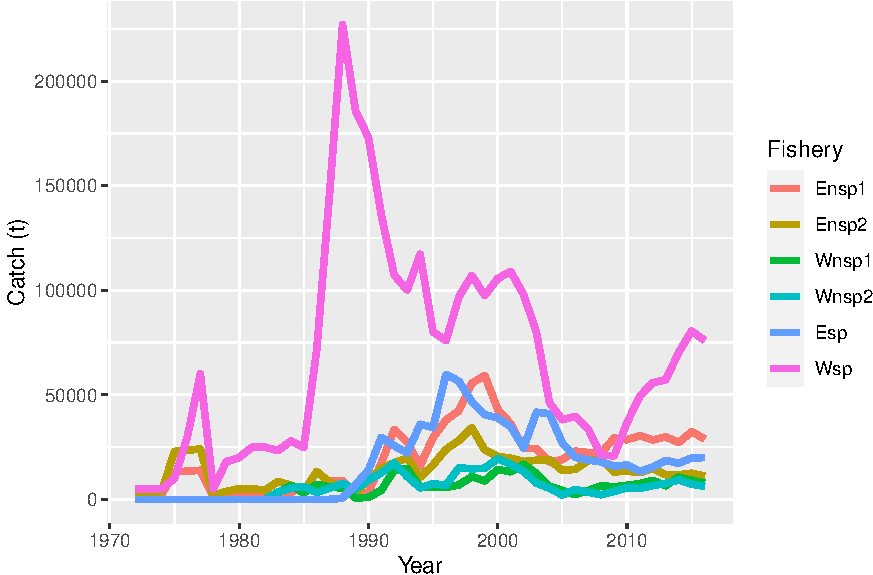
\includegraphics{_main_files/figure-latex/input_catches-1.pdf}

\begin{Shaded}
\begin{Highlighting}[]
\FunctionTok{ggplot}\NormalTok{(summary}\SpecialCharTok{$}\NormalTok{obs\_year\_df, }\FunctionTok{aes}\NormalTok{(}\AttributeTok{x =}\NormalTok{ year, }\AttributeTok{y =}\NormalTok{ observation, }\AttributeTok{col =}\NormalTok{ observation, }\AttributeTok{size =}\NormalTok{ active)) }\SpecialCharTok{+}
  \FunctionTok{geom\_point}\NormalTok{() }\SpecialCharTok{+}
  \FunctionTok{guides}\NormalTok{(}\AttributeTok{colour =} \StringTok{"none"}\NormalTok{, }\AttributeTok{size =} \StringTok{"none"}\NormalTok{)}
\end{Highlighting}
\end{Shaded}

\begin{verbatim}
## Warning: Removed 509 rows containing missing values (`geom_point()`).
\end{verbatim}

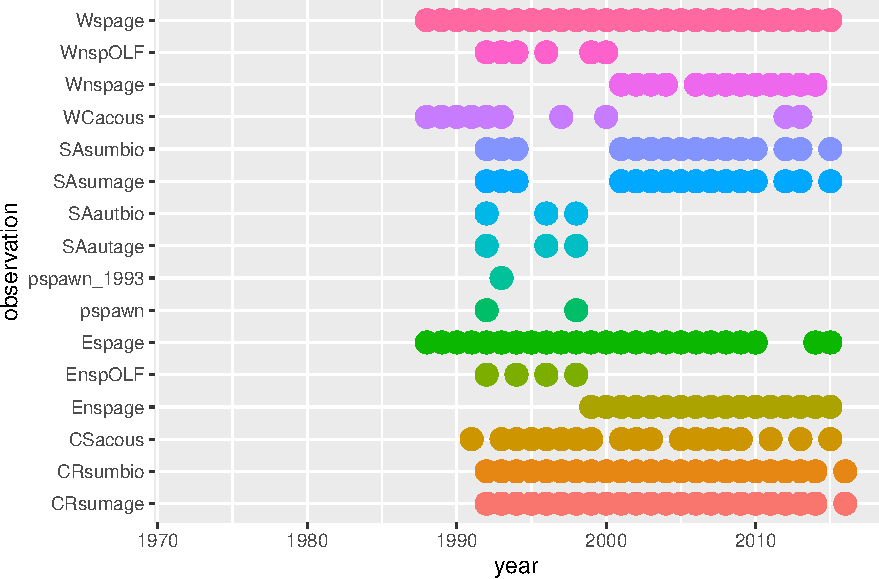
\includegraphics{_main_files/figure-latex/input_observations-1.pdf}

\begin{Shaded}
\begin{Highlighting}[]
\FunctionTok{kable}\NormalTok{(}\AttributeTok{x =}\NormalTok{ summary}\SpecialCharTok{$}\NormalTok{time\_step\_df, }\AttributeTok{caption =} \StringTok{"Annual cycle"}\NormalTok{)}
\end{Highlighting}
\end{Shaded}

\begin{table}

\caption{(\#tab:$annual_cycle$)Annual cycle}
\centering
\begin{tabular}[t]{l|l|l|l|l|l}
\hline
Time-step & Processes (type) & age\_size\_W\_male (assumed growth) & age\_size\_E\_male (assumed growth) & age\_size\_W\_female (assumed growth) & age\_size\_E\_female (assumed growth)\\
\hline
Oct\_Nov & Wrtn (transition\_category), Ertn (transition\_category), Instant\_mortality (mortality\_instantaneous) & 0.25 & 0.25 & 0.25 & 0.25\\
\hline
Dec\_Mar & recruit\_W (recruitment\_beverton\_holt), recruit\_E (recruitment\_beverton\_holt), Instant\_mortality (mortality\_instantaneous) & 0.6 & 0.6 & 0.6 & 0.6\\
\hline
Apr\_Jun & Whome (transition\_category), Instant\_mortality (mortality\_instantaneous) & 0.9 & 0.9 & 0.9 & 0.9\\
\hline
End\_Jun & Wspmg (transition\_category), Espmg (transition\_category) & 0.9 & 0.9 & 0.9 & 0.9\\
\hline
Jul\_Sep & Ageing (ageing), Instant\_mortality (mortality\_instantaneous), SSB\_E (derived-quantity 0.5), SSB\_W (derived-quantity 0.5) & 0.0 & 0.0 & 0.0 & 0.0\\
\hline
\end{tabular}
\end{table}

\begin{Shaded}
\begin{Highlighting}[]
\FunctionTok{kable}\NormalTok{(}\AttributeTok{x =}\NormalTok{ summary}\SpecialCharTok{$}\NormalTok{full\_category\_df, }\AttributeTok{caption =} \StringTok{"Category information"}\NormalTok{)}
\end{Highlighting}
\end{Shaded}

\begin{table}

\caption{\label{tab:categories}Category information}
\centering
\begin{tabular}[t]{l|l|l|l}
\hline
Category & AgeLength & LengthWeight & Distribution\\
\hline
male.west.sa & age\_size\_W\_male (von\_bertalanffy) & Length\_weight (basic) & normal\\
\hline
male.east.cr & age\_size\_E\_male (von\_bertalanffy) & Length\_weight (basic) & normal\\
\hline
male.west.cr & age\_size\_W\_male (von\_bertalanffy) & Length\_weight (basic) & normal\\
\hline
male.west.wc & age\_size\_W\_male (von\_bertalanffy) & Length\_weight (basic) & normal\\
\hline
male.east.cs & age\_size\_E\_male (von\_bertalanffy) & Length\_weight (basic) & normal\\
\hline
female.west.sa & age\_size\_W\_female (von\_bertalanffy) & Length\_weight (basic) & normal\\
\hline
female.east.cr & age\_size\_E\_female (von\_bertalanffy) & Length\_weight (basic) & normal\\
\hline
female.west.cr & age\_size\_W\_female (von\_bertalanffy) & Length\_weight (basic) & normal\\
\hline
female.west.wc & age\_size\_W\_female (von\_bertalanffy) & Length\_weight (basic) & normal\\
\hline
female.east.cs & age\_size\_E\_female (von\_bertalanffy) & Length\_weight (basic) & normal\\
\hline
\end{tabular}
\end{table}

\begin{Shaded}
\begin{Highlighting}[]
\FunctionTok{kable}\NormalTok{(}\AttributeTok{x =}\NormalTok{ summary}\SpecialCharTok{$}\NormalTok{estimate\_df, }\AttributeTok{caption =} \StringTok{"Estimate summary"}\NormalTok{)}
\end{Highlighting}
\end{Shaded}

\begin{table}

\caption{\label{tab:estimates}Estimate summary}
\centering
\begin{tabular}[t]{l|l|l|l|l}
\hline
label & same & prior & lower\_bound & upper\_bound\\
\hline
CSacousq & - & lognormal & 0.01 & 4.53\\
\hline
WCacousq & - & lognormal & 0.01 & 3.35\\
\hline
CRsumq & - & lognormal & 0.016 & 0.51\\
\hline
SAsumq & - & lognormal & 0.020 & 0.51\\
\hline
SAautq & - & lognormal & 0.020 & 0.51\\
\hline
CR\_process\_error & - & uniform & 0.0 & 1\\
\hline
SA\_process\_error & - & uniform & 0.0 & 1\\
\hline
B0\_E\_with\_total\_log\_b0\_prior & - & uniform & 12.6 & 16.2\\
\hline
B0\_W\_with\_proportion\_prior & - & beta & 0.11 & 0.59\\
\hline
YCS\_E & - & lognormal & 0.06 0.06 0.06 0.06 0.06 0.06 0.06 0.06 0.06 0.06 0.06 0.06 0.06 0.06 0.06 0.06 0.06 0.06 0.06 0.06 0.06 0.06 0.06 0.06 0.06 0.06 0.06 0.06 0.06 0.06 0.06 0.06 0.06 0.06 0.06 0.06 0.06 0.06 0.06 0.06 & 8.60 8.60 8.60 8.60 8.60 8.60 8.60 8.60 8.60 8.60 8.60 8.60 8.60 8.60 8.60 8.60 8.60 8.60 8.60 8.60 8.60 8.60 8.60 8.60 8.60 8.60 8.60 8.60 8.60 8.60 8.60 8.60 8.60 8.60 8.60 8.60 8.60 8.60 8.60 8.60\\
\hline
YCS\_W & - & lognormal & 0.06 0.06 0.06 0.06 0.06 0.06 0.06 0.06 0.06 0.06 0.06 0.06 0.06 0.06 0.06 0.06 0.06 0.06 0.06 0.06 0.06 0.06 0.06 0.06 0.06 0.06 0.06 0.06 0.06 0.06 0.06 0.06 0.06 0.06 0.06 0.06 0.06 0.06 0.06 0.06 & 8.60 8.60 8.60 8.60 8.60 8.60 8.60 8.60 8.60 8.60 8.60 8.60 8.60 8.60 8.60 8.60 8.60 8.60 8.60 8.60 8.60 8.60 8.60 8.60 8.60 8.60 8.60 8.60 8.60 8.60 8.60 8.60 8.60 8.60 8.60 8.60 8.60 8.60 8.60 8.60\\
\hline
M\_male\_x0 & - & uniform & 5.1 & 9.1\\
\hline
M\_male\_y0 & - & uniform & 0.01 & 0.30\\
\hline
M\_male\_y1 & - & uniform & 0.5 & 2.0\\
\hline
M\_male\_y2 & - & uniform & 0.5 & 2.0\\
\hline
M\_female\_x0 & - & uniform & 5.1 & 9.1\\
\hline
M\_female\_y0 & - & uniform & 0.01 & 0.30\\
\hline
M\_female\_y1 & - & uniform & 0.5 & 2.0\\
\hline
M\_female\_y2 & - & uniform & 0.5 & 2.0\\
\hline
sel\_Whome & - & uniform & 0.01 0.01 0.01 0 0 0 0 1 & 1 1 1 1 1 1 1 1\\
\hline
sel\_Espmg\_male & - & uniform & 0 0 0 0 0 0 0 0 & 1 1 1 1 1 1 1 1\\
\hline
sel\_Wspmg\_male & - & uniform & 0 0 0 0 0 0 0 0 & 1 1 1 1 1 1 1 1\\
\hline
sel\_Espmg\_female & - & uniform & 0 0 0 0 0 0 0 0.6 & 1 1 1 1 1 1 1 1\\
\hline
sel\_Wspmg\_female & - & uniform & 0 0 0 0 0 0 0 0.6 & 1 1 1 1 1 1 1 1\\
\hline
Enspsl\_mu & - & uniform & 64 & 84\\
\hline
Enspsl\_s\_l & - & uniform & 4 & 44\\
\hline
Enspsl\_s\_r & - & uniform & 4 & 44\\
\hline
Wnspsl\_mu & - & uniform & 64 & 84\\
\hline
Wnspsl\_s\_l & - & uniform & 4 & 44\\
\hline
Wnspsl\_s\_r & - & uniform & 4 & 44\\
\hline
Espsl\_a50 & - & uniform & 6 & 80\\
\hline
Espsl\_ato95 & - & uniform & 4 & 60\\
\hline
Wspsl\_shift\_param & - & normal\_by\_stdev & -10.24 & 2.24\\
\hline
CRsl\_mu & - & uniform & 64 & 84\\
\hline
CRsl\_s\_l & - & uniform & 4 & 44\\
\hline
CRsl\_s\_r & - & uniform & 4 & 44\\
\hline
SAsl\_mu & - & uniform & 64 & 84\\
\hline
SAsl\_s\_l & - & uniform & 4 & 44\\
\hline
SAsl\_s\_r & - & uniform & 4 & 44\\
\hline
\end{tabular}
\end{table}

\hypertarget{mpd-summaries}{%
\chapter{MPD summaries}\label{mpd-summaries}}

\hypertarget{single-model-output}{%
\section{Single Model Output}\label{single-model-output}}

\begin{Shaded}
\begin{Highlighting}[]
\NormalTok{file\_name }\OtherTok{=} \FunctionTok{system.file}\NormalTok{(}\StringTok{"extdata"}\NormalTok{,}\StringTok{"SimpleTestModel"}\NormalTok{, }
                        \StringTok{"estimate.log"}\NormalTok{, }\AttributeTok{package =} \StringTok{"r4Casal2"}\NormalTok{, }\AttributeTok{mustWork =} \ConstantTok{TRUE}\NormalTok{)}
\NormalTok{mpd }\OtherTok{=} \FunctionTok{extract.mpd}\NormalTok{(}\AttributeTok{file =}\NormalTok{ file\_name)}
\end{Highlighting}
\end{Shaded}

\hypertarget{model-convergence}{%
\subsection{Model Convergence}\label{model-convergence}}

There are a range of appproaches for checking your model has converged. The approaches we will be working through include checking the hessian is positive definite, checking parameters are not running to bounds and reestimate with random starting locations.

When estimating models in Casal2, it is recommended to have the following report included

\begin{Shaded}
\begin{Highlighting}[]
\ExtensionTok{@report}\NormalTok{ covariance\_matrix}
\BuiltInTok{type}\NormalTok{ covariance\_matrix}
\CommentTok{\#\# or the Hessian}
\ExtensionTok{@report}\NormalTok{ hessian\_matrix}
\BuiltInTok{type}\NormalTok{ hessian\_matrix}
\end{Highlighting}
\end{Shaded}

When estimation is complete and you have read in the Casal2 output using \texttt{Casal2::extract.mpd()}.

\begin{Shaded}
\begin{Highlighting}[]
\CommentTok{\# file name}
\NormalTok{mpd\_file\_name }\OtherTok{=} \FunctionTok{system.file}\NormalTok{(}\StringTok{"extdata"}\NormalTok{, }\StringTok{"PosteriorPredictiveChecks"}\NormalTok{,}\StringTok{"estimate.log"}\NormalTok{, }
                            \AttributeTok{package =} \StringTok{"r4Casal2"}\NormalTok{, }\AttributeTok{mustWork =} \ConstantTok{TRUE}\NormalTok{)}
\CommentTok{\# read in output}
\NormalTok{mpd }\OtherTok{=} \FunctionTok{extract.mpd}\NormalTok{(}\AttributeTok{file =}\NormalTok{ mpd\_file\_name)}
\CommentTok{\# is covariance symmetric}
\FunctionTok{isSymmetric}\NormalTok{(mpd}\SpecialCharTok{$}\NormalTok{covar}\SpecialCharTok{$}\NormalTok{covariance\_matrix)}
\CommentTok{\# is hessian invertable}
\FunctionTok{is\_matrix\_invertable}\NormalTok{(mpd}\SpecialCharTok{$}\NormalTok{hess}\SpecialCharTok{$}\NormalTok{hessian\_matrix)}
\CommentTok{\# check high correlations}
\NormalTok{correlation\_matrix }\OtherTok{=} \FunctionTok{cov2cor}\NormalTok{(mpd}\SpecialCharTok{$}\NormalTok{covar}\SpecialCharTok{$}\NormalTok{covariance\_matrix)}
\NormalTok{corr\_df }\OtherTok{=} \FunctionTok{get\_high\_correlations}\NormalTok{(}\AttributeTok{correlation\_matrix =}\NormalTok{ correlation\_matrix, }\AttributeTok{max\_correlation =} \FloatTok{0.8}\NormalTok{, }
                      \AttributeTok{labels =} \FunctionTok{names}\NormalTok{(mpd}\SpecialCharTok{$}\NormalTok{estimate\_value}\SpecialCharTok{$}\NormalTok{values))}
\NormalTok{corr\_df}\SpecialCharTok{$}\NormalTok{correlation }\OtherTok{=} \FunctionTok{round}\NormalTok{(corr\_df}\SpecialCharTok{$}\NormalTok{correlation, }\DecValTok{3}\NormalTok{)}
\end{Highlighting}
\end{Shaded}

\begin{Shaded}
\begin{Highlighting}[]
\FunctionTok{kable}\NormalTok{(}\AttributeTok{x =}\NormalTok{ corr\_df[,}\FunctionTok{c}\NormalTok{(}\StringTok{"correlation"}\NormalTok{, }\StringTok{"row\_param"}\NormalTok{, }\StringTok{"col\_param"}\NormalTok{)], }
      \AttributeTok{caption =} \StringTok{"Correlated Parameters"}\NormalTok{)}
\end{Highlighting}
\end{Shaded}

\begin{table}

\caption{(\#tab:$correlated_params$)Correlated Parameters}
\centering
\begin{tabular}[t]{r|l|l}
\hline
correlation & row\_param & col\_param\\
\hline
-0.974 & process[Recruitment].b0 & catchability[chatTANq].q\\
\hline
0.830 & selectivity[chatTANSel].mu & selectivity[chatTANSel].sigma\_l\\
\hline
0.951 & selectivity[eastFSel].mu & selectivity[eastFSel].sigma\_l\\
\hline
0.925 & selectivity[westFSel].mu & selectivity[westFSel].sigma\_l\\
\hline
0.810 & process[Recruitment].ycs\_values\{1978\} & process[Recruitment].ycs\_values\{1979\}\\
\hline
0.818 & process[Recruitment].ycs\_values\{1979\} & process[Recruitment].ycs\_values\{1980\}\\
\hline
0.827 & process[Recruitment].ycs\_values\{1980\} & process[Recruitment].ycs\_values\{1981\}\\
\hline
0.831 & process[Recruitment].ycs\_values\{1981\} & process[Recruitment].ycs\_values\{1982\}\\
\hline
0.835 & process[Recruitment].ycs\_values\{1982\} & process[Recruitment].ycs\_values\{1983\}\\
\hline
\end{tabular}
\end{table}

You will want to try remove high correlations from the covariance to help estimation and MCMC simulations. We recommend you explore parameter transformations to remove high correlations or alternative parameterisations.

Once these are satisfied you will have more confidence in your standard errors, in addition to being able to run MCMC run mode.

Another useful convergence diagnostic is re-estimating Casal2 with difference starting locations. The function used for this is \texttt{?generate.starting.pars}. This will read a Casal2 config file that contains all the \texttt{@estimate} definitions are generate a bunch of random starting values in the format of useable for \texttt{-i} in Casal2. Below is some example R code of running Casal2 from R with randomly generated starting values.

\begin{Shaded}
\begin{Highlighting}[]
\NormalTok{working\_dir }\OtherTok{=} \StringTok{"Directory to Casal output"}
\DocumentationTok{\#\# generate starting values}
\NormalTok{start\_pars }\OtherTok{=} \FunctionTok{generate.starting.pars}\NormalTok{(}\AttributeTok{path =}\NormalTok{ working\_dir, }
                                    \AttributeTok{estimation\_csl2\_file  =} \StringTok{"estimation.csl2"}\NormalTok{,}
                                    \AttributeTok{par\_file\_name =} \StringTok{"starting\_pars.out"}\NormalTok{)}
\DocumentationTok{\#\# re{-}run Casal2}
\NormalTok{current\_dir }\OtherTok{=} \FunctionTok{getwd}\NormalTok{()}
\FunctionTok{setwd}\NormalTok{(working\_dir)}
\FunctionTok{system2}\NormalTok{(}\AttributeTok{command =} \StringTok{"casal2"}\NormalTok{, }\AttributeTok{args =} \StringTok{"{-}e {-}o multi\_start\_pars.par {-}i starting\_pars.out"}\NormalTok{,}
        \AttributeTok{stdout =} \StringTok{"multi\_start.log"}\NormalTok{,}
        \AttributeTok{stderr =} \StringTok{"multi\_start.err"}\NormalTok{, }\AttributeTok{wait=}\ConstantTok{TRUE}\NormalTok{)}
\FunctionTok{system2}\NormalTok{(}\AttributeTok{command =} \StringTok{"casal2"}\NormalTok{, }\AttributeTok{args =} \StringTok{"{-}r {-}i starting\_pars.out"}\NormalTok{,}
        \AttributeTok{stdout =} \StringTok{"multi\_start\_init.log"}\NormalTok{,}
        \AttributeTok{stderr =} \StringTok{"multi\_start\_init.err"}\NormalTok{, }\AttributeTok{wait=}\ConstantTok{TRUE}\NormalTok{)}
\FunctionTok{setwd}\NormalTok{(current\_dir)}

\DocumentationTok{\#\# read in jitter\_start run}
\NormalTok{multi\_est }\OtherTok{=} \FunctionTok{extract.mpd}\NormalTok{(}\StringTok{"multi\_start.log"}\NormalTok{, }\AttributeTok{path =}\NormalTok{ working\_dir)}
\NormalTok{multi\_run }\OtherTok{=} \FunctionTok{extract.mpd}\NormalTok{(}\StringTok{"multi\_start\_init.log"}\NormalTok{, }\AttributeTok{path =}\NormalTok{ working\_dir)}
\DocumentationTok{\#\# check if any didn\textquotesingle{}t converge}

\DocumentationTok{\#\# plot SSBS}
\NormalTok{ssb\_df }\OtherTok{=} \FunctionTok{get\_derived\_quantities}\NormalTok{(multi\_est)}
\FunctionTok{ggplot}\NormalTok{(ssb\_df, }\FunctionTok{aes}\NormalTok{(}\AttributeTok{x =}\NormalTok{ years, }\AttributeTok{y =}\NormalTok{ values, }\AttributeTok{col =}\NormalTok{ par\_set, }\AttributeTok{linetype =}\NormalTok{ par\_set)) }\SpecialCharTok{+}
  \FunctionTok{geom\_line}\NormalTok{(}\AttributeTok{size =} \FloatTok{1.5}\NormalTok{) }\SpecialCharTok{+}
  \FunctionTok{labs}\NormalTok{(}\AttributeTok{x =} \StringTok{"Years"}\NormalTok{,}\AttributeTok{y =} \StringTok{"SSB"}\NormalTok{, }\AttributeTok{linetype =} \StringTok{"Starting}\SpecialCharTok{\textbackslash{}n}\StringTok{values"}\NormalTok{, }\AttributeTok{col =} \StringTok{"Starting}\SpecialCharTok{\textbackslash{}n}\StringTok{values"}\NormalTok{)}
\NormalTok{ssb\_df }\OtherTok{=} \FunctionTok{get\_derived\_quantities}\NormalTok{(multi\_run)}
\FunctionTok{ggplot}\NormalTok{(ssb\_df, }\FunctionTok{aes}\NormalTok{(}\AttributeTok{x =}\NormalTok{ years, }\AttributeTok{y =}\NormalTok{ values, }\AttributeTok{col =}\NormalTok{ par\_set, }\AttributeTok{linetype =}\NormalTok{ par\_set)) }\SpecialCharTok{+}
  \FunctionTok{geom\_line}\NormalTok{(}\AttributeTok{size =} \FloatTok{1.5}\NormalTok{) }\SpecialCharTok{+}
  \FunctionTok{labs}\NormalTok{(}\AttributeTok{x =} \StringTok{"Years"}\NormalTok{,}\AttributeTok{y =} \StringTok{"SSB"}\NormalTok{, }\AttributeTok{linetype =} \StringTok{"Starting}\SpecialCharTok{\textbackslash{}n}\StringTok{values"}\NormalTok{, }\AttributeTok{col =} \StringTok{"Starting}\SpecialCharTok{\textbackslash{}n}\StringTok{values"}\NormalTok{)}

\DocumentationTok{\#\# get aggregated objective functions}
\NormalTok{obj }\OtherTok{=} \FunctionTok{aggregate\_objective\_report}\NormalTok{(}\AttributeTok{model =}\NormalTok{ multi\_est)}
\FunctionTok{head}\NormalTok{(obj)}
\end{Highlighting}
\end{Shaded}

A useful diagnostic that is encouraged to explore is to run Casal2 as an age-structured population model (ASPM) \citep{MINTEVERA2017114, CARVALHO2021105959}. This is useful for asking the following question ``do we need to know the variability in recruitment to get the ``correct'' trends in relative abundance and the absolute scale of the model?'' The diagnostic is run following these steps
1. Estimate the full integrated model
2. Fix selectivity parameters at MPD values from step 2
3. Turn off recruitment variability i.e., assume \(R_0\) for all years
4. fit the model (ASPM) to the indices of abundance only. Just estimating \(R_0\), \(q\) etc.
5. fit the above model again but estimate YCS parameters (ASPMdev)
6. fit the model again with the recruitment deviates set equal to the MPD values from the integrated model (ASPMfix)

This runs will help you explore the fit and production assumptions in the data. The idea is to understand what parameters are informing what population signals and how perhaps identify misspecifications. For more information on this diagnostic we recommend users read \citet{MINTEVERA2017114}.

\hypertarget{data-weighting}{%
\subsection{Data Weighting}\label{data-weighting}}

Some pseudo r code to help with data weighting according to \citet{francis2011data} with multinomial data.

\begin{Shaded}
\begin{Highlighting}[]
\NormalTok{working\_dir }\OtherTok{=} \StringTok{"Directory to Casal output"}
\NormalTok{reweight\_folder }\OtherTok{=} \StringTok{"Reweight"}
\DocumentationTok{\#\# Don\textquotesingle{}t always want to re{-}run this code}
\ControlFlowTok{if}\NormalTok{(}\ConstantTok{FALSE}\NormalTok{) \{}
\NormalTok{  weights }\OtherTok{=} \FunctionTok{run\_automatic\_reweighting}\NormalTok{(}\AttributeTok{config\_dir =}\NormalTok{ working\_dir,}
                                      \AttributeTok{config\_filename =} \StringTok{"config.csl2"}\NormalTok{,}
                                      \AttributeTok{weighting\_folder\_name =}\NormalTok{ reweight\_folder,}
                                      \AttributeTok{mpd\_file\_name =} \StringTok{"estimate.log"}\NormalTok{,}
                                      \AttributeTok{n\_loops =} \DecValTok{3}\NormalTok{, }
                                      \AttributeTok{approximate\_single\_year\_obs =}\NormalTok{ T)}
  \FunctionTok{saveRDS}\NormalTok{(weights, }\AttributeTok{file =} \FunctionTok{file.path}\NormalTok{(working\_dir, reweight\_folder, }\StringTok{"Weights.RDS"}\NormalTok{))}
\NormalTok{\}}
\DocumentationTok{\#\# get reweighted MPDs to observe the effect}
\NormalTok{MPD\_list }\OtherTok{=} \FunctionTok{extract\_reweighted\_mpds}\NormalTok{(}\FunctionTok{file.path}\NormalTok{(working\_dir,reweight\_folder))}

\DocumentationTok{\#\# plot SSBs}
\FunctionTok{plot\_derived\_quantities}\NormalTok{(MPD\_list)}
\FunctionTok{plot\_fishery}\NormalTok{(MPD\_list, }\AttributeTok{quantity =} \StringTok{"exploitation"}\NormalTok{)}
\FunctionTok{plot\_recruitment}\NormalTok{(MPD\_list, }\AttributeTok{quantity =} \StringTok{"standardised\_recruitment\_multipliers"}\NormalTok{)}
\end{Highlighting}
\end{Shaded}

\hypertarget{model-quantities}{%
\subsection{Model quantities}\label{model-quantities}}

\hypertarget{fishing-pressures}{%
\subsubsection*{Fishing Pressures}\label{fishing-pressures}}
\addcontentsline{toc}{subsubsection}{Fishing Pressures}

Below illustrates code to plot fishing pressure, but you can also easily adapt the code to plot catches. One thing to note, is Casal2 will report both \texttt{exploitation\_rate} (actual a proportion also called harvest rate) and \texttt{fishing\_pressures}. For models that only have a single fishery per time-step and area these quantities will be the same. If there are multiple fisheries interacting with the partition in the same time-step then these quantities will differ. Fishing pressure is the maximum exploitation applied to the partition for that time-step. See the Casal2 user manual for more detail on the difference. \texttt{exploitation\_rate} reported is just
\[
\frac{catch}{vulnerable}
\]

Some R-code used to summarise fishing pressures.

\begin{Shaded}
\begin{Highlighting}[]
\NormalTok{file\_name }\OtherTok{=} \FunctionTok{system.file}\NormalTok{(}\StringTok{"extdata"}\NormalTok{, }\StringTok{"SimpleTestModel"}\NormalTok{, }\StringTok{"estimate.log"}\NormalTok{, }
                        \AttributeTok{package =} \StringTok{"r4Casal2"}\NormalTok{, }\AttributeTok{mustWork =} \ConstantTok{TRUE}\NormalTok{)}
\NormalTok{mpd }\OtherTok{=} \FunctionTok{extract.mpd}\NormalTok{(}\AttributeTok{file =}\NormalTok{ file\_name)}
\CommentTok{\# Report labels}
\CommentTok{\# names(mpd) }
\CommentTok{\# plot fishing pressures}
\NormalTok{fishery\_info }\OtherTok{=} \FunctionTok{get\_fisheries}\NormalTok{(mpd)}
\FunctionTok{head}\NormalTok{(fishery\_info)}
\CommentTok{\# Note this will print both fishing pressure and exploitation}
\NormalTok{my\_plot }\OtherTok{=} \FunctionTok{ggplot}\NormalTok{(fishery\_info, }\FunctionTok{aes}\NormalTok{(}\AttributeTok{x =}\NormalTok{ year, }\AttributeTok{y =}\NormalTok{ exploitation, }\AttributeTok{col =}\NormalTok{ fishery, }\AttributeTok{linetype =}\NormalTok{ fishery)) }\SpecialCharTok{+}
                   \FunctionTok{geom\_line}\NormalTok{(}\AttributeTok{size =}\DecValTok{2}\NormalTok{)}
\NormalTok{my\_plot}
\end{Highlighting}
\end{Shaded}

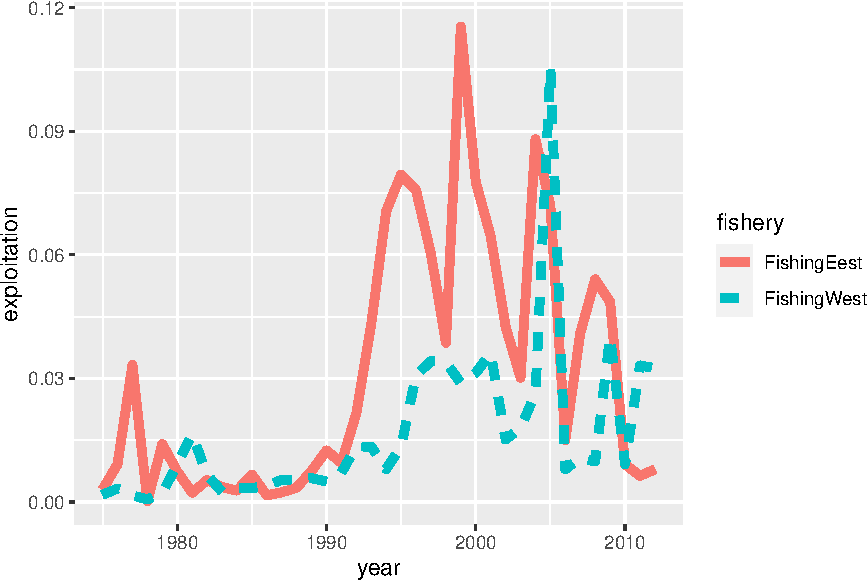
\includegraphics{_main_files/figure-latex/pressures-1.pdf}
Flexibility using standard ggplot functions

\begin{Shaded}
\begin{Highlighting}[]
\CommentTok{\# you can add adjust it as you please, for example if you want 3 panels for each fishery}
\NormalTok{my\_plot }\SpecialCharTok{+} 
  \FunctionTok{facet\_wrap}\NormalTok{(}\SpecialCharTok{\textasciitilde{}}\NormalTok{fishery) }\SpecialCharTok{+} 
  \FunctionTok{theme}\NormalTok{(}\AttributeTok{axis.text.x =} \FunctionTok{element\_text}\NormalTok{(}\AttributeTok{angle =} \DecValTok{90}\NormalTok{))}
\end{Highlighting}
\end{Shaded}

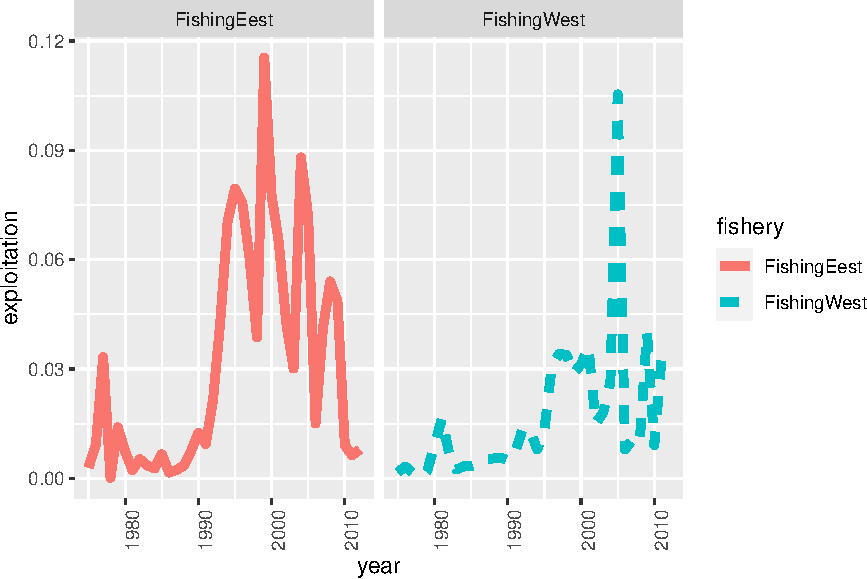
\includegraphics{_main_files/figure-latex/pressures_alt-1.pdf}

\begin{Shaded}
\begin{Highlighting}[]
\CommentTok{\# Adjust ylim and add a reference limit}
\NormalTok{my\_plot }\SpecialCharTok{+} \FunctionTok{ylim}\NormalTok{(}\DecValTok{0}\NormalTok{,}\FloatTok{0.09}\NormalTok{) }\SpecialCharTok{+} \FunctionTok{geom\_hline}\NormalTok{(}\AttributeTok{yintercept =} \FloatTok{0.05}\NormalTok{, }\AttributeTok{linetype =} \StringTok{"dashed"}\NormalTok{)}
\end{Highlighting}
\end{Shaded}

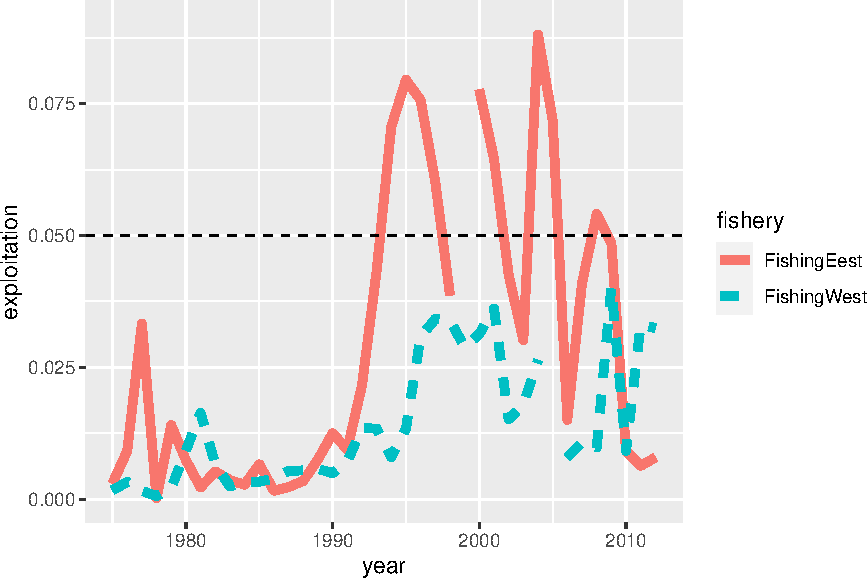
\includegraphics{_main_files/figure-latex/pressures_alt_again-1.pdf}
\#\#\#\# SSBs \{-\}

\begin{Shaded}
\begin{Highlighting}[]
\CommentTok{\# get SSB and recruit}
\NormalTok{ssb\_df }\OtherTok{=} \FunctionTok{get\_dqs}\NormalTok{(mpd)}
\NormalTok{ssb\_df}\SpecialCharTok{$}\NormalTok{model\_year }\OtherTok{=}\NormalTok{ ssb\_df}\SpecialCharTok{$}\NormalTok{years}
\NormalTok{recruit\_df }\OtherTok{=} \FunctionTok{get\_BH\_recruitment}\NormalTok{(mpd)}
\CommentTok{\# merge these two data frames}
\NormalTok{joint\_df }\OtherTok{=} \FunctionTok{right\_join}\NormalTok{(}\AttributeTok{x =}\NormalTok{ ssb\_df, }\AttributeTok{y =}\NormalTok{ recruit\_df, }\AttributeTok{by =} \FunctionTok{c}\NormalTok{(}\StringTok{"model\_year"}\NormalTok{, }\StringTok{"par\_set"}\NormalTok{))}
\DocumentationTok{\#\# for multi{-}stock models, you will need to also join by stock id}
\NormalTok{joint\_df}\SpecialCharTok{$}\NormalTok{percent\_b0 }\OtherTok{=}\NormalTok{ joint\_df}\SpecialCharTok{$}\NormalTok{values }\SpecialCharTok{/}\NormalTok{ joint\_df}\SpecialCharTok{$}\NormalTok{b0 }\SpecialCharTok{*} \DecValTok{100}
\DocumentationTok{\#\# plot percent B0}
\FunctionTok{ggplot}\NormalTok{(joint\_df, }\FunctionTok{aes}\NormalTok{(}\AttributeTok{x =}\NormalTok{ years, }\AttributeTok{y =}\NormalTok{ percent\_b0)) }\SpecialCharTok{+}
  \FunctionTok{geom\_line}\NormalTok{(}\AttributeTok{size =} \DecValTok{2}\NormalTok{) }\SpecialCharTok{+}
  \FunctionTok{ylim}\NormalTok{(}\DecValTok{0}\NormalTok{,}\ConstantTok{NA}\NormalTok{) }\SpecialCharTok{+}
  \FunctionTok{labs}\NormalTok{(}\AttributeTok{x =} \StringTok{"Year"}\NormalTok{, }\AttributeTok{y =} \FunctionTok{expression}\NormalTok{(}\FunctionTok{paste}\NormalTok{(S[t], }\StringTok{" / "}\NormalTok{, S[}\DecValTok{0}\NormalTok{], }\StringTok{" (\%)"}\NormalTok{))) }\SpecialCharTok{+}
  \FunctionTok{geom\_hline}\NormalTok{(}\AttributeTok{yintercept =} \DecValTok{40}\NormalTok{, }\AttributeTok{col =} \StringTok{"darkgreen"}\NormalTok{, }\AttributeTok{linetype =} \StringTok{"dashed"}\NormalTok{, }\AttributeTok{size =} \FloatTok{1.5}\NormalTok{) }\SpecialCharTok{+}
  \FunctionTok{geom\_label}\NormalTok{(}\AttributeTok{x =} \DecValTok{1900}\NormalTok{, }\AttributeTok{y =} \DecValTok{40}\NormalTok{, }\AttributeTok{label =} \StringTok{"Target"}\NormalTok{) }\SpecialCharTok{+}
  \FunctionTok{geom\_hline}\NormalTok{(}\AttributeTok{yintercept =} \DecValTok{20}\NormalTok{, }\AttributeTok{col =} \StringTok{"orange"}\NormalTok{, }\AttributeTok{linetype =} \StringTok{"dashed"}\NormalTok{, }\AttributeTok{size =} \FloatTok{1.5}\NormalTok{) }\SpecialCharTok{+}
  \FunctionTok{geom\_label}\NormalTok{(}\AttributeTok{x =} \DecValTok{1900}\NormalTok{, }\AttributeTok{y =} \DecValTok{20}\NormalTok{, }\AttributeTok{label =} \StringTok{"Soft"}\NormalTok{) }\SpecialCharTok{+}
  \FunctionTok{geom\_hline}\NormalTok{(}\AttributeTok{yintercept =} \DecValTok{10}\NormalTok{, }\AttributeTok{col =} \StringTok{"red"}\NormalTok{, }\AttributeTok{linetype =} \StringTok{"dashed"}\NormalTok{, }\AttributeTok{size =} \FloatTok{1.5}\NormalTok{) }\SpecialCharTok{+}
  \FunctionTok{geom\_label}\NormalTok{(}\AttributeTok{x =} \DecValTok{1900}\NormalTok{, }\AttributeTok{y =} \DecValTok{10}\NormalTok{, }\AttributeTok{label =} \StringTok{"Hard"}\NormalTok{)}\SpecialCharTok{+}
  \FunctionTok{ggtitle}\NormalTok{(}\StringTok{"Percent B0"}\NormalTok{) }\SpecialCharTok{+}
  \FunctionTok{theme\_classic}\NormalTok{() }\SpecialCharTok{+}
  \FunctionTok{theme}\NormalTok{(}\AttributeTok{legend.position =} \StringTok{"bottom"}\NormalTok{, }
        \AttributeTok{axis.text =} \FunctionTok{element\_text}\NormalTok{(}\AttributeTok{size =} \DecValTok{16}\NormalTok{), }
        \AttributeTok{axis.title =} \FunctionTok{element\_text}\NormalTok{(}\AttributeTok{size =} \DecValTok{16}\NormalTok{),}
        \AttributeTok{strip.text =} \FunctionTok{element\_text}\NormalTok{(}\AttributeTok{size=}\DecValTok{16}\NormalTok{),}
        \AttributeTok{title=}\FunctionTok{element\_blank}\NormalTok{(),}
        \AttributeTok{legend.text =} \FunctionTok{element\_text}\NormalTok{(}\AttributeTok{size=}\DecValTok{16}\NormalTok{))}
\end{Highlighting}
\end{Shaded}

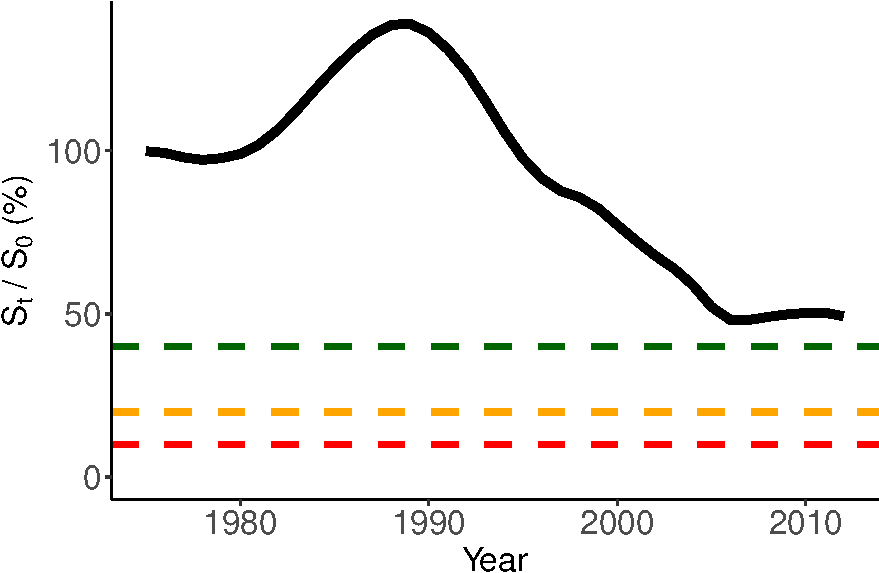
\includegraphics{_main_files/figure-latex/ssbs-1.pdf}

\hypertarget{plotting-selectivities}{%
\subsubsection{Plotting selectivities}\label{plotting-selectivities}}

\begin{Shaded}
\begin{Highlighting}[]
\NormalTok{selectivity\_df }\OtherTok{=} \FunctionTok{get\_selectivities}\NormalTok{(}\AttributeTok{model =}\NormalTok{ mpd)}
\FunctionTok{ggplot}\NormalTok{(selectivity\_df, }\FunctionTok{aes}\NormalTok{(}\AttributeTok{x =}\NormalTok{ bin, }\AttributeTok{y =}\NormalTok{ selectivity, }\AttributeTok{col =}\NormalTok{ selectivity\_label)) }\SpecialCharTok{+}
  \FunctionTok{geom\_line}\NormalTok{(}\AttributeTok{size =} \FloatTok{1.5}\NormalTok{) }\SpecialCharTok{+}
  \FunctionTok{facet\_wrap}\NormalTok{(}\SpecialCharTok{\textasciitilde{}}\NormalTok{selectivity\_label)}
\end{Highlighting}
\end{Shaded}

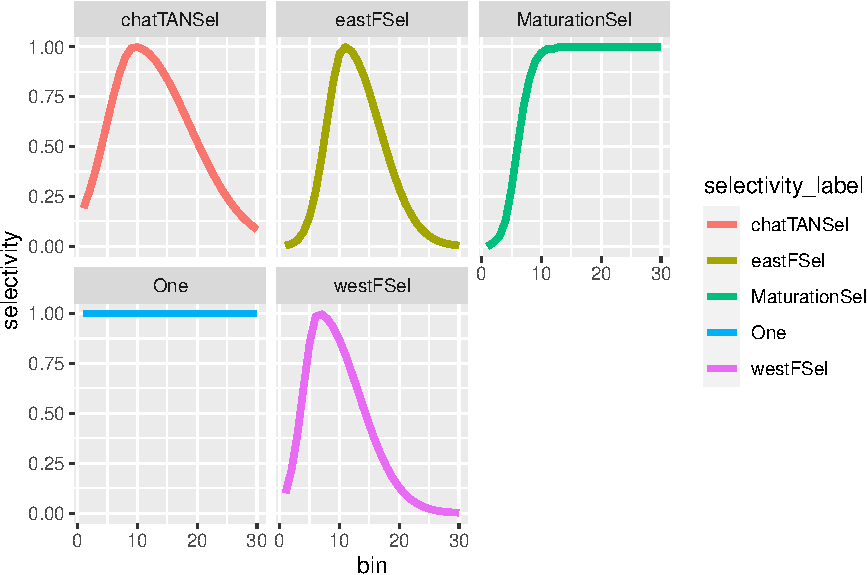
\includegraphics{_main_files/figure-latex/selectivities_mpd-1.pdf}
\#\#\#\# Growth \{-\}

\begin{Shaded}
\begin{Highlighting}[]
\NormalTok{growth\_df }\OtherTok{=} \FunctionTok{get\_growth}\NormalTok{(mpd)}
\FunctionTok{head}\NormalTok{(growth\_df)}
\end{Highlighting}
\end{Shaded}

\begin{verbatim}
##   age year time_step cvs_by_age mean_length_at_age mean_weight_at_age            label par_set
## 1   1 1975     step1        0.1            29.6178        0.000143136 age_length_step1       1
## 2   2 1975     step1        0.1            44.7450        0.000555816 age_length_step1       1
## 3   3 1975     step1        0.1            55.5000        0.001128550 age_length_step1       1
## 4   4 1975     step1        0.1            63.8482        0.001789010 age_length_step1       1
## 5   5 1975     step1        0.1            70.5854        0.002488050 age_length_step1       1
## 6   6 1975     step1        0.1            76.1440        0.003192290 age_length_step1       1
\end{verbatim}

\begin{Shaded}
\begin{Highlighting}[]
\DocumentationTok{\#\# if time{-}varying or type data summarise mean length and weight by year}
\NormalTok{avg\_summarises }\OtherTok{=}\NormalTok{ growth\_df }\SpecialCharTok{\%\textgreater{}\%} \FunctionTok{group\_by}\NormalTok{(year) }\SpecialCharTok{\%\textgreater{}\%} \FunctionTok{summarise}\NormalTok{(}
  \AttributeTok{mean\_length =} \FunctionTok{mean}\NormalTok{(mean\_length\_at\_age), }
  \AttributeTok{mean\_weight =} \FunctionTok{mean}\NormalTok{(mean\_weight\_at\_age))}

\FunctionTok{ggplot}\NormalTok{(avg\_summarises, }\FunctionTok{aes}\NormalTok{(}\AttributeTok{x =}\NormalTok{ year, }\AttributeTok{y =}\NormalTok{ mean\_length)) }\SpecialCharTok{+}
  \FunctionTok{geom\_point}\NormalTok{(}\AttributeTok{size =}\DecValTok{2}\NormalTok{) }\SpecialCharTok{+}
  \FunctionTok{geom\_line}\NormalTok{(}\AttributeTok{col =} \StringTok{"gray60"}\NormalTok{, }\AttributeTok{linetype =} \StringTok{"dashed"}\NormalTok{) }\SpecialCharTok{+}
  \FunctionTok{ylab}\NormalTok{(}\StringTok{"Mean length (cm)"}\NormalTok{) }\SpecialCharTok{+}
  \FunctionTok{theme\_classic}\NormalTok{()}
\end{Highlighting}
\end{Shaded}

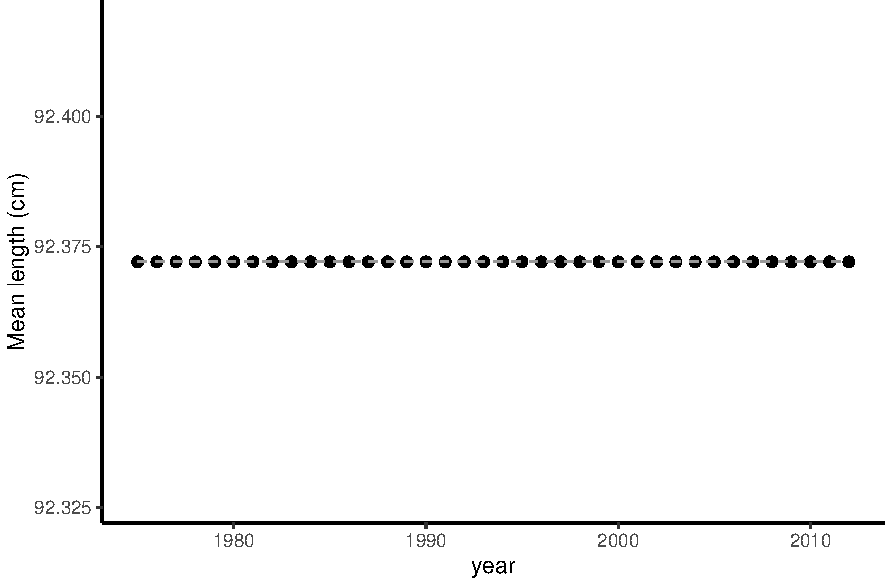
\includegraphics{_main_files/figure-latex/growth_df-1.pdf}

\begin{Shaded}
\begin{Highlighting}[]
\FunctionTok{ggplot}\NormalTok{(avg\_summarises, }\FunctionTok{aes}\NormalTok{(}\AttributeTok{x =}\NormalTok{ year, }\AttributeTok{y =}\NormalTok{ mean\_weight }\SpecialCharTok{*} \DecValTok{1000}\NormalTok{)) }\SpecialCharTok{+}
  \FunctionTok{geom\_point}\NormalTok{(}\AttributeTok{size =}\DecValTok{2}\NormalTok{) }\SpecialCharTok{+}
  \FunctionTok{geom\_line}\NormalTok{(}\AttributeTok{col =} \StringTok{"gray60"}\NormalTok{, }\AttributeTok{linetype =} \StringTok{"dashed"}\NormalTok{) }\SpecialCharTok{+}
  \FunctionTok{ylab}\NormalTok{(}\StringTok{"Mean weight (kg)"}\NormalTok{) }\SpecialCharTok{+}
  \FunctionTok{theme\_classic}\NormalTok{() }
\end{Highlighting}
\end{Shaded}

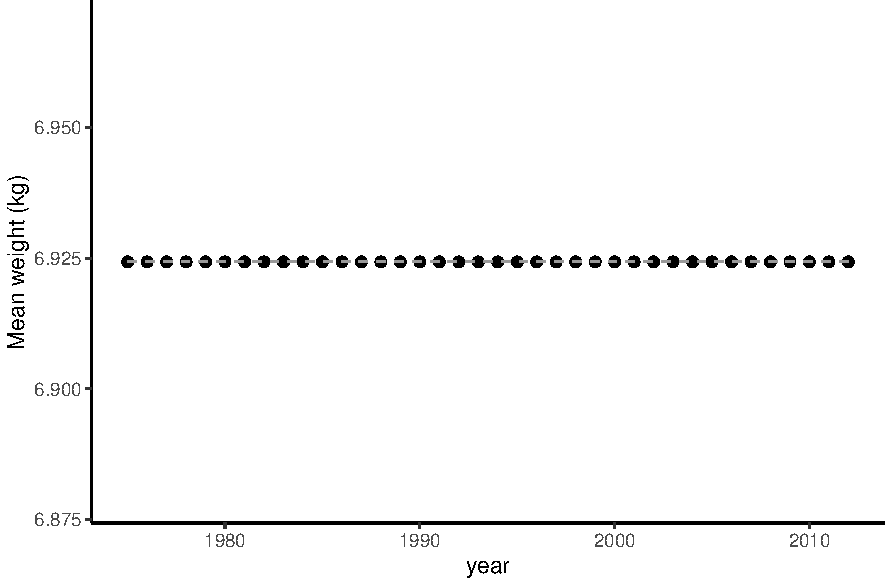
\includegraphics{_main_files/figure-latex/growth_df-2.pdf}

\begin{Shaded}
\begin{Highlighting}[]
\DocumentationTok{\#\# if not time{-}varying just pick one year to plot}
\FunctionTok{ggplot}\NormalTok{(growth\_df }\SpecialCharTok{\%\textgreater{}\%} \FunctionTok{filter}\NormalTok{(year }\SpecialCharTok{==} \DecValTok{1990}\NormalTok{)) }\SpecialCharTok{+}
  \FunctionTok{geom\_line}\NormalTok{(}\FunctionTok{aes}\NormalTok{(}\AttributeTok{x =}\NormalTok{ age, }\AttributeTok{y =}\NormalTok{ mean\_length\_at\_age, }\AttributeTok{col =}\NormalTok{ time\_step, }\AttributeTok{linetype =}\NormalTok{ time\_step), }\AttributeTok{size =} \FloatTok{1.2}\NormalTok{) }\SpecialCharTok{+}
  \FunctionTok{labs}\NormalTok{(}\AttributeTok{x =} \StringTok{"Age"}\NormalTok{, }\AttributeTok{y =} \StringTok{"Length (cm)"}\NormalTok{, }\AttributeTok{col =} \StringTok{"Time{-}step"}\NormalTok{)}
\end{Highlighting}
\end{Shaded}

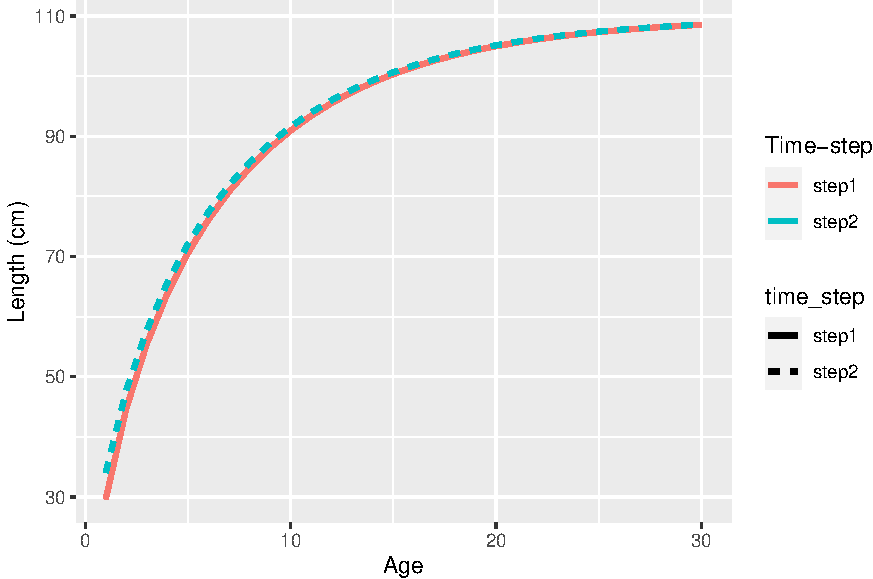
\includegraphics{_main_files/figure-latex/growth_by_time_step_df-1.pdf}

\hypertarget{plotting-fits}{%
\subsection{Plotting Fits}\label{plotting-fits}}

\hypertarget{relative-abundance}{%
\subsubsection*{Relative abundance}\label{relative-abundance}}
\addcontentsline{toc}{subsubsection}{Relative abundance}

\begin{Shaded}
\begin{Highlighting}[]
\DocumentationTok{\#\# define a palette}
\NormalTok{obs\_palette }\OtherTok{\textless{}{-}} \FunctionTok{c}\NormalTok{(}\StringTok{"\#E69F00"}\NormalTok{, }\StringTok{"\#56B4E9"}\NormalTok{,}\StringTok{"\#009E73"}\NormalTok{)}
\FunctionTok{names}\NormalTok{(obs\_palette) }\OtherTok{=} \FunctionTok{c}\NormalTok{(}\StringTok{"Observed"}\NormalTok{, }\StringTok{"Predicted"}\NormalTok{,}\StringTok{"Pearson\textquotesingle{}s Residuals"}\NormalTok{)}
\DocumentationTok{\#\# get abundance data frames}
\NormalTok{abundance\_obs }\OtherTok{=} \FunctionTok{get\_abundance\_observations}\NormalTok{(mpd)}
\NormalTok{abundance\_obs\_label }\OtherTok{=} \FunctionTok{unique}\NormalTok{((abundance\_obs}\SpecialCharTok{$}\NormalTok{observation\_label))}

\DocumentationTok{\#\# plot observed vs fitted}
\FunctionTok{ggplot}\NormalTok{(abundance\_obs, }\FunctionTok{aes}\NormalTok{(}\AttributeTok{x =}\NormalTok{ year)) }\SpecialCharTok{+}
    \FunctionTok{geom\_line}\NormalTok{(}\FunctionTok{aes}\NormalTok{(}\AttributeTok{y =}\NormalTok{ expected, }\AttributeTok{col =} \StringTok{"Predicted"}\NormalTok{), }\AttributeTok{size =} \FloatTok{1.2}\NormalTok{, }
              \AttributeTok{linetype =} \StringTok{"dashed"}\NormalTok{) }\SpecialCharTok{+}
    \FunctionTok{geom\_point}\NormalTok{(}\FunctionTok{aes}\NormalTok{(}\AttributeTok{y =}\NormalTok{ expected, }\AttributeTok{col =} \StringTok{"Predicted"}\NormalTok{), }\AttributeTok{size =} \FloatTok{2.5}\NormalTok{) }\SpecialCharTok{+}
    \FunctionTok{geom\_errorbar}\NormalTok{(}\FunctionTok{aes}\NormalTok{(}\AttributeTok{ymin =}\NormalTok{ L\_CI, }\AttributeTok{ymax =}\NormalTok{ U\_CI, }\AttributeTok{col =} \StringTok{"Observed"}\NormalTok{), }
                  \AttributeTok{width=}\NormalTok{.}\DecValTok{5}\NormalTok{, }\AttributeTok{position =} \FunctionTok{position\_dodge}\NormalTok{(}\AttributeTok{width=}\FloatTok{0.9}\NormalTok{)) }\SpecialCharTok{+}
    \FunctionTok{geom\_point}\NormalTok{(}\FunctionTok{aes}\NormalTok{(}\AttributeTok{y =}\NormalTok{ observed, }\AttributeTok{col =} \StringTok{"Observed"}\NormalTok{), }\AttributeTok{size =} \FloatTok{2.5}\NormalTok{) }\SpecialCharTok{+}
    \FunctionTok{labs}\NormalTok{(}\AttributeTok{x =} \StringTok{"Year"}\NormalTok{, }\AttributeTok{y =} \StringTok{"Relative index"}\NormalTok{, }\AttributeTok{color =} \StringTok{""}\NormalTok{) }\SpecialCharTok{+}
    \FunctionTok{ylim}\NormalTok{(}\DecValTok{0}\NormalTok{,}\ConstantTok{NA}\NormalTok{) }\SpecialCharTok{+}
    \FunctionTok{theme\_classic}\NormalTok{() }\SpecialCharTok{+}
    \FunctionTok{facet\_wrap}\NormalTok{(}\SpecialCharTok{\textasciitilde{}}\NormalTok{observation\_label, }\AttributeTok{ncol =} \DecValTok{1}\NormalTok{, }\AttributeTok{scales =} \StringTok{"free\_y"}\NormalTok{) }\SpecialCharTok{+}
    \FunctionTok{theme}\NormalTok{(}\AttributeTok{legend.position =} \StringTok{"bottom"}\NormalTok{, }
          \AttributeTok{axis.text =} \FunctionTok{element\_text}\NormalTok{(}\AttributeTok{size =} \DecValTok{14}\NormalTok{), }
          \AttributeTok{axis.title =} \FunctionTok{element\_text}\NormalTok{(}\AttributeTok{size =} \DecValTok{14}\NormalTok{),}
          \AttributeTok{strip.text =} \FunctionTok{element\_text}\NormalTok{(}\AttributeTok{size=}\DecValTok{14}\NormalTok{),}
          \AttributeTok{legend.text =} \FunctionTok{element\_text}\NormalTok{(}\AttributeTok{size=}\DecValTok{14}\NormalTok{)) }\SpecialCharTok{+}
    \FunctionTok{scale\_color\_manual}\NormalTok{(}\AttributeTok{values =}\NormalTok{ obs\_palette[}\DecValTok{1}\SpecialCharTok{:}\DecValTok{2}\NormalTok{])}
\end{Highlighting}
\end{Shaded}

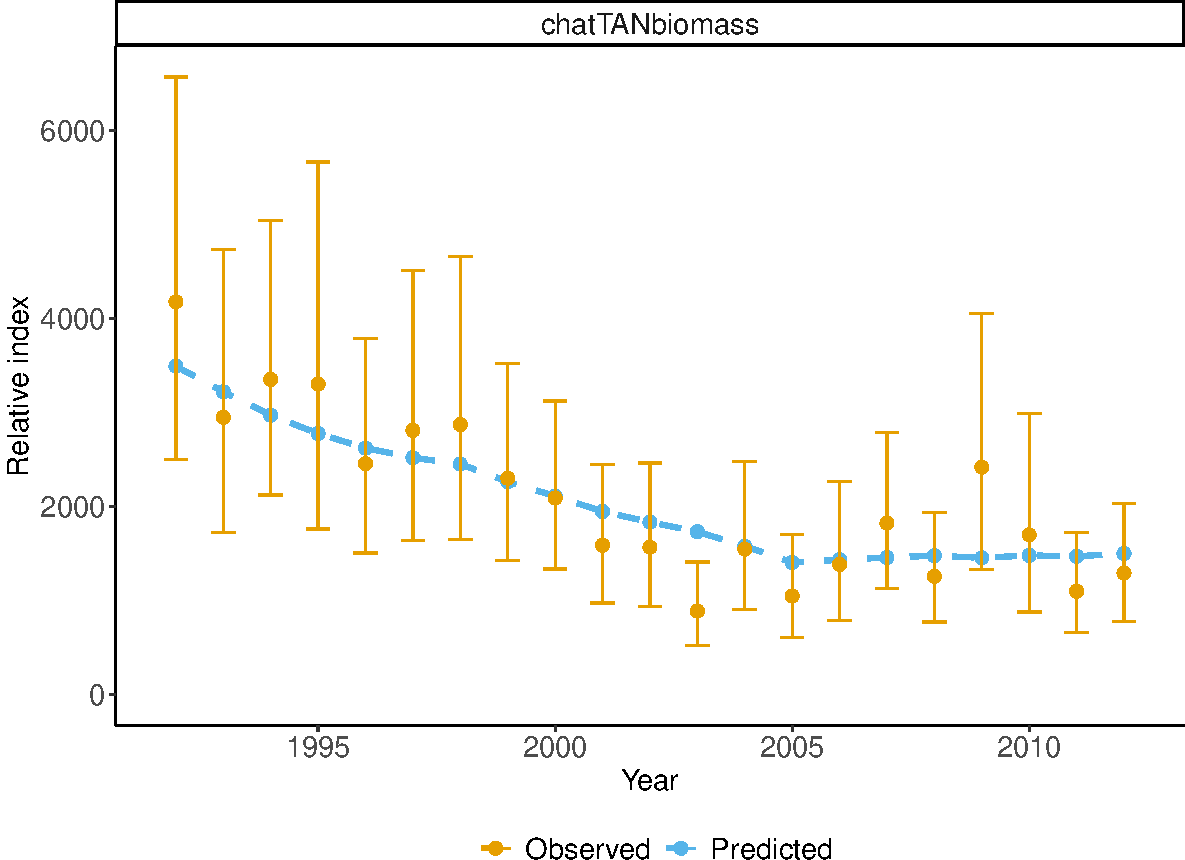
\includegraphics{_main_files/figure-latex/plot_relative_index-1.pdf}

\begin{Shaded}
\begin{Highlighting}[]
\DocumentationTok{\#\# Plot pearsons residuals}
\FunctionTok{ggplot}\NormalTok{(abundance\_obs, }\FunctionTok{aes}\NormalTok{(}\AttributeTok{x =}\NormalTok{ year)) }\SpecialCharTok{+}
  \FunctionTok{geom\_point}\NormalTok{(}\FunctionTok{aes}\NormalTok{(}\AttributeTok{y =}\NormalTok{ pearsons\_residuals, }\AttributeTok{col =} \StringTok{"Pearson\textquotesingle{}s Residuals"}\NormalTok{), }
             \AttributeTok{size =} \DecValTok{2}\NormalTok{) }\SpecialCharTok{+}
  \FunctionTok{geom\_smooth}\NormalTok{(}\FunctionTok{aes}\NormalTok{(}\AttributeTok{y =}\NormalTok{ pearsons\_residuals, }\AttributeTok{col =} \StringTok{"Pearson\textquotesingle{}s Residuals"}\NormalTok{, }
                  \AttributeTok{fill =} \StringTok{"Pearson\textquotesingle{}s Residuals"}\NormalTok{), }\AttributeTok{size =} \FloatTok{1.5}\NormalTok{, }\AttributeTok{alpha =} \FloatTok{0.4}\NormalTok{,}
              \AttributeTok{linetype =} \StringTok{"dashed"}\NormalTok{) }\SpecialCharTok{+}
  \FunctionTok{labs}\NormalTok{(}\AttributeTok{x =} \StringTok{"Age"}\NormalTok{, }\AttributeTok{y =} \StringTok{"Pearson\textquotesingle{}s Residuals"}\NormalTok{, }\AttributeTok{fill =} \StringTok{""}\NormalTok{, }\AttributeTok{col =} \StringTok{""}\NormalTok{) }\SpecialCharTok{+}
  \FunctionTok{geom\_hline}\NormalTok{(}\AttributeTok{yintercept =} \DecValTok{0}\NormalTok{, }\AttributeTok{col =} \StringTok{"\#999999"}\NormalTok{, }\AttributeTok{linetype =} \StringTok{"dashed"}\NormalTok{, }
             \AttributeTok{size =} \FloatTok{1.2}\NormalTok{) }\SpecialCharTok{+}
  \FunctionTok{geom\_hline}\NormalTok{(}\AttributeTok{yintercept =} \FunctionTok{c}\NormalTok{(}\SpecialCharTok{{-}}\DecValTok{2}\NormalTok{,}\DecValTok{2}\NormalTok{), }\AttributeTok{col =} \StringTok{"red"}\NormalTok{, }\AttributeTok{linetype =} \StringTok{"dashed"}\NormalTok{, }
             \AttributeTok{size =} \FloatTok{1.2}\NormalTok{) }\SpecialCharTok{+} 
  \FunctionTok{facet\_wrap}\NormalTok{(}\SpecialCharTok{\textasciitilde{}}\NormalTok{observation\_label, }\AttributeTok{ncol =} \DecValTok{4}\NormalTok{) }\SpecialCharTok{+}
  \CommentTok{\#ylim(3,{-}3) +}
  \FunctionTok{theme\_classic}\NormalTok{() }\SpecialCharTok{+}
  \FunctionTok{facet\_wrap}\NormalTok{(}\SpecialCharTok{\textasciitilde{}}\NormalTok{observation\_label, }\AttributeTok{ncol =} \DecValTok{1}\NormalTok{, }\AttributeTok{scales =} \StringTok{"free\_y"}\NormalTok{) }\SpecialCharTok{+}
  \FunctionTok{list}\NormalTok{(}\FunctionTok{theme}\NormalTok{(}\AttributeTok{legend.position =} \StringTok{"bottom"}\NormalTok{, }
        \AttributeTok{axis.text =} \FunctionTok{element\_text}\NormalTok{(}\AttributeTok{size =} \DecValTok{14}\NormalTok{), }
        \AttributeTok{axis.title =} \FunctionTok{element\_text}\NormalTok{(}\AttributeTok{size =} \DecValTok{14}\NormalTok{),}
        \AttributeTok{strip.text =} \FunctionTok{element\_text}\NormalTok{(}\AttributeTok{size=}\DecValTok{14}\NormalTok{),}
        \AttributeTok{legend.text =} \FunctionTok{element\_text}\NormalTok{(}\AttributeTok{size=}\DecValTok{14}\NormalTok{)),}
  \FunctionTok{scale\_color\_manual}\NormalTok{(}\AttributeTok{values =}\NormalTok{ obs\_pallete[}\DecValTok{3}\NormalTok{]),}
  \FunctionTok{scale\_fill\_manual}\NormalTok{(}\AttributeTok{values =}\NormalTok{ obs\_pallete[}\DecValTok{3}\NormalTok{]))}
\end{Highlighting}
\end{Shaded}

\begin{verbatim}
## `geom_smooth()` using method = 'loess' and formula = 'y ~ x'
\end{verbatim}

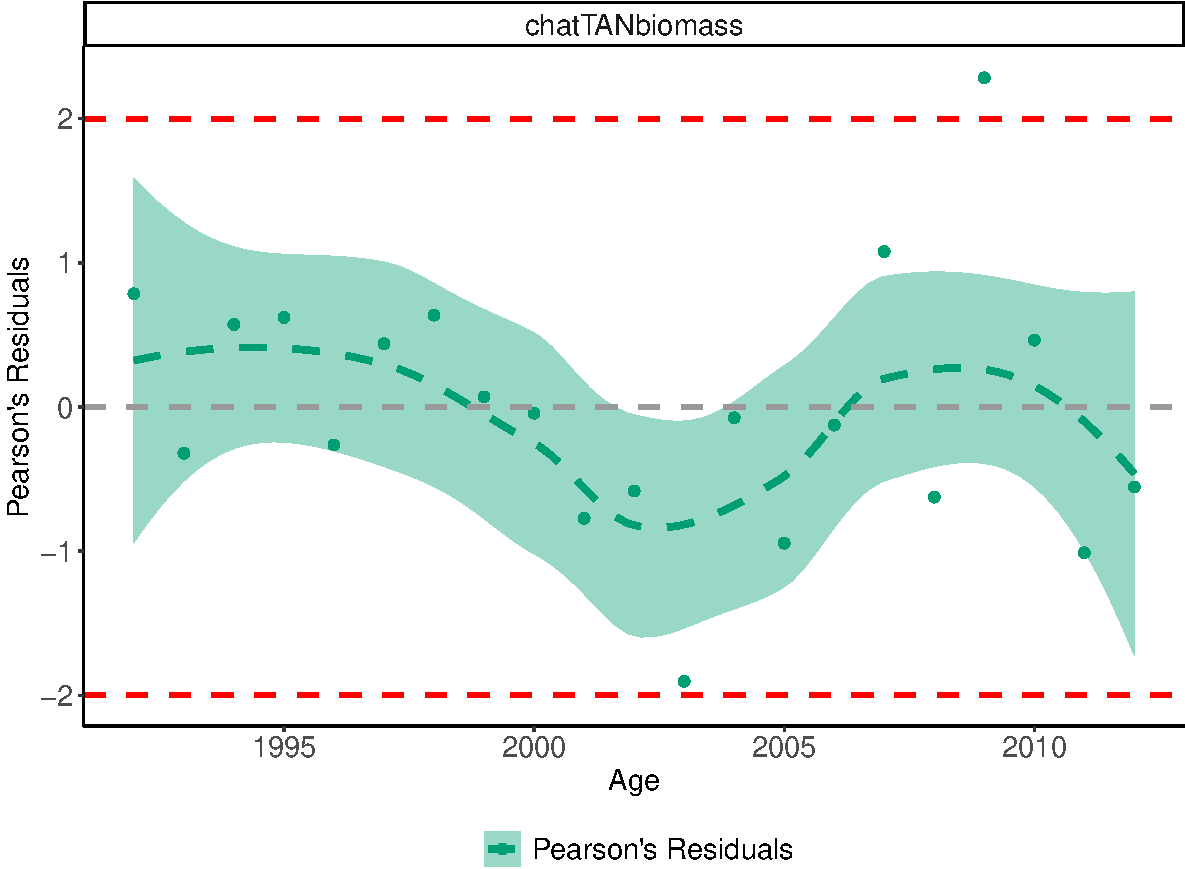
\includegraphics{_main_files/figure-latex/plot_resid_index-1.pdf}

\begin{Shaded}
\begin{Highlighting}[]
\DocumentationTok{\#\# complete a Wald{-}Wolfowitz Runs Test}
\DocumentationTok{\#\# are residuals a random sequence}
\FunctionTok{runs\_test\_residuals}\NormalTok{(abundance\_obs}\SpecialCharTok{$}\NormalTok{pearsons\_residuals)}
\end{Highlighting}
\end{Shaded}

\begin{verbatim}
## $siglim
## [1] -2.340038  2.340038
## 
## $p.runs
## [1] 0.556
\end{verbatim}

\begin{Shaded}
\begin{Highlighting}[]
\DocumentationTok{\#\# seem fine i.e. not rejecting Null hypothesis }
\DocumentationTok{\#\# H0: "The order of the data is random "}
\end{Highlighting}
\end{Shaded}

\hypertarget{age-composition}{%
\subsubsection*{Age composition}\label{age-composition}}
\addcontentsline{toc}{subsubsection}{Age composition}

\begin{Shaded}
\begin{Highlighting}[]
\DocumentationTok{\#\# define a palette}
\NormalTok{comp\_obs }\OtherTok{=} \FunctionTok{get\_composition\_observations}\NormalTok{(mpd)}
\FunctionTok{unique}\NormalTok{(comp\_obs}\SpecialCharTok{$}\NormalTok{observation\_label)}
\end{Highlighting}
\end{Shaded}

\begin{verbatim}
## [1] "chatTANage" "chatOBSwst" "chatOBSest"
\end{verbatim}

\begin{Shaded}
\begin{Highlighting}[]
\DocumentationTok{\#\# just plot one of them}
\DocumentationTok{\#\# and the first 12 years}
\NormalTok{this\_obs }\OtherTok{=}\NormalTok{ comp\_obs }\SpecialCharTok{\%\textgreater{}\%} \FunctionTok{filter}\NormalTok{(observation\_label }\SpecialCharTok{==} \StringTok{"chatTANage"}\NormalTok{)}
\NormalTok{years\_to\_plot }\OtherTok{=} \FunctionTok{unique}\NormalTok{(this\_obs}\SpecialCharTok{$}\NormalTok{year)[}\DecValTok{1}\SpecialCharTok{:}\DecValTok{12}\NormalTok{]}
\DocumentationTok{\#\# calculate effective N for plot}
\NormalTok{this\_obs }\OtherTok{=}\NormalTok{ this\_obs }\SpecialCharTok{\%\textgreater{}\%} \FunctionTok{group\_by}\NormalTok{(year, observation\_label) }\SpecialCharTok{\%\textgreater{}\%} 
  \FunctionTok{mutate}\NormalTok{(}\AttributeTok{Nassumed =} \FunctionTok{mean}\NormalTok{(adjusted\_error))}
\NormalTok{  this\_obs}\SpecialCharTok{$}\NormalTok{label }\OtherTok{=} \FunctionTok{paste0}\NormalTok{(this\_obs}\SpecialCharTok{$}\NormalTok{year, }\StringTok{" N = "}\NormalTok{, }\FunctionTok{round}\NormalTok{(this\_obs}\SpecialCharTok{$}\NormalTok{Nassumed,}\DecValTok{1}\NormalTok{))}

\FunctionTok{ggplot}\NormalTok{(this\_obs, }\FunctionTok{aes}\NormalTok{(}\AttributeTok{x =}\NormalTok{ age)) }\SpecialCharTok{+}
  \FunctionTok{geom\_line}\NormalTok{(}\FunctionTok{aes}\NormalTok{(}\AttributeTok{y =}\NormalTok{ expected, }\AttributeTok{col =} \StringTok{"Predicted"}\NormalTok{), }\AttributeTok{size =} \FloatTok{1.5}\NormalTok{) }\SpecialCharTok{+}
  \FunctionTok{geom\_point}\NormalTok{(}\FunctionTok{aes}\NormalTok{(}\AttributeTok{y =}\NormalTok{ observed, }\AttributeTok{col =} \StringTok{"Observed"}\NormalTok{), }\AttributeTok{size =} \FloatTok{2.5}\NormalTok{) }\SpecialCharTok{+}
  \FunctionTok{labs}\NormalTok{(}\AttributeTok{x =} \StringTok{"Age"}\NormalTok{, }\AttributeTok{y =} \StringTok{"Proportions"}\NormalTok{) }\SpecialCharTok{+}
  \FunctionTok{facet\_wrap}\NormalTok{(}\SpecialCharTok{\textasciitilde{}}\NormalTok{label, }\AttributeTok{ncol =} \DecValTok{4}\NormalTok{) }\SpecialCharTok{+}
  \FunctionTok{ggtitle}\NormalTok{(}\StringTok{"chatTANage"}\NormalTok{) }\SpecialCharTok{+}
  \FunctionTok{theme\_classic}\NormalTok{() }\SpecialCharTok{+}
  \FunctionTok{theme}\NormalTok{(}\AttributeTok{legend.position =} \StringTok{"bottom"}\NormalTok{, }
        \AttributeTok{axis.text =} \FunctionTok{element\_text}\NormalTok{(}\AttributeTok{size =} \DecValTok{14}\NormalTok{), }
        \AttributeTok{axis.title =} \FunctionTok{element\_text}\NormalTok{(}\AttributeTok{size =} \DecValTok{14}\NormalTok{),}
        \AttributeTok{strip.text =} \FunctionTok{element\_text}\NormalTok{(}\AttributeTok{size=}\DecValTok{14}\NormalTok{),}
        \AttributeTok{legend.text =} \FunctionTok{element\_text}\NormalTok{(}\AttributeTok{size=}\DecValTok{14}\NormalTok{)) }\SpecialCharTok{+}
  \FunctionTok{scale\_color\_manual}\NormalTok{(}\AttributeTok{values =}\NormalTok{ obs\_palette[}\DecValTok{1}\SpecialCharTok{:}\DecValTok{2}\NormalTok{])}
\end{Highlighting}
\end{Shaded}

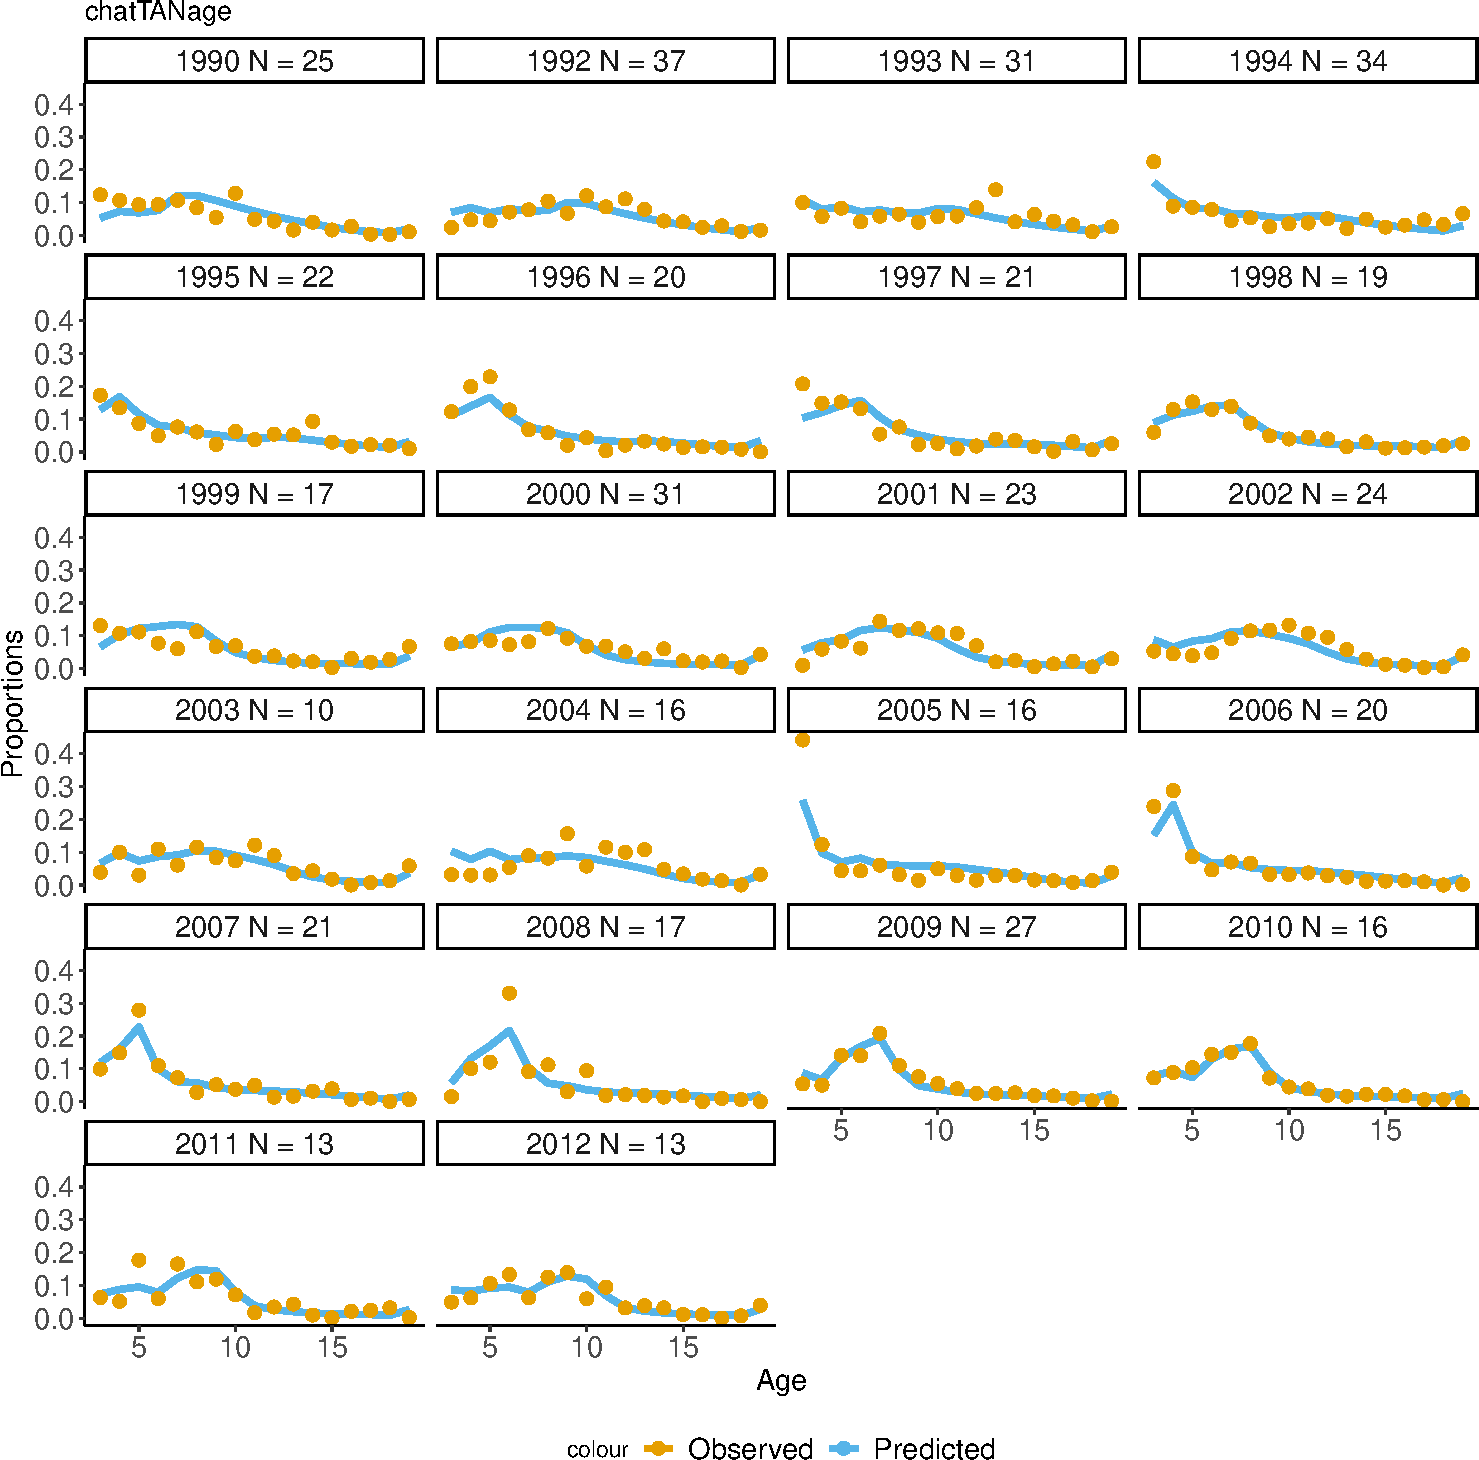
\includegraphics{_main_files/figure-latex/plot_comp_fit-1.pdf}

\begin{Shaded}
\begin{Highlighting}[]
\NormalTok{mean\_age\_df }\OtherTok{=} \FunctionTok{get\_composition\_mean\_bin}\NormalTok{(mpd)}
\NormalTok{n\_obs }\OtherTok{=} \FunctionTok{unique}\NormalTok{(mean\_age\_df}\SpecialCharTok{$}\NormalTok{observation\_label)}
\DocumentationTok{\#\# create a nice plot with separate axis}
\FunctionTok{ggplot}\NormalTok{(mean\_age\_df, }\FunctionTok{aes}\NormalTok{(}\AttributeTok{x =}\NormalTok{ year, }\AttributeTok{col =}\NormalTok{ observation\_label)) }\SpecialCharTok{+}
  \FunctionTok{geom\_errorbar}\NormalTok{(}\FunctionTok{aes}\NormalTok{(}\AttributeTok{ymin =}\NormalTok{ Oy}\DecValTok{{-}2}\SpecialCharTok{*}\NormalTok{SEy, }\AttributeTok{ymax =}\NormalTok{ Oy }\SpecialCharTok{+} \DecValTok{2}\SpecialCharTok{*}\NormalTok{SEy), }\AttributeTok{width=}\NormalTok{.}\DecValTok{5}\NormalTok{, }
                \AttributeTok{position =} \FunctionTok{position\_dodge}\NormalTok{(}\AttributeTok{width=}\DecValTok{0}\NormalTok{)) }\SpecialCharTok{+}
  \FunctionTok{geom\_point}\NormalTok{(}\FunctionTok{aes}\NormalTok{(}\AttributeTok{y =}\NormalTok{ Oy), }\AttributeTok{position =} \FunctionTok{position\_dodge}\NormalTok{(}\AttributeTok{width=}\FloatTok{0.9}\NormalTok{)) }\SpecialCharTok{+}
  \FunctionTok{geom\_line}\NormalTok{(}\FunctionTok{aes}\NormalTok{(}\AttributeTok{y =}\NormalTok{ Ey), }\AttributeTok{linetype =} \StringTok{"dashed"}\NormalTok{) }\SpecialCharTok{+}
  \FunctionTok{labs}\NormalTok{(}\AttributeTok{x =} \StringTok{"Years"}\NormalTok{,}\AttributeTok{y =} \StringTok{"Mean age (+{-} 2 SE)"}\NormalTok{) }\SpecialCharTok{+}
  \FunctionTok{facet\_wrap}\NormalTok{(}\SpecialCharTok{\textasciitilde{}}\NormalTok{observation\_label, }\AttributeTok{nrow =} \FunctionTok{length}\NormalTok{(n\_obs))  }\SpecialCharTok{+}
  \FunctionTok{theme}\NormalTok{(}\AttributeTok{legend.position =} \StringTok{"bottom"}\NormalTok{, }
        \AttributeTok{axis.text =} \FunctionTok{element\_text}\NormalTok{(}\AttributeTok{size =} \DecValTok{14}\NormalTok{), }
        \AttributeTok{axis.title =} \FunctionTok{element\_text}\NormalTok{(}\AttributeTok{size =} \DecValTok{14}\NormalTok{),}
        \AttributeTok{strip.text =} \FunctionTok{element\_text}\NormalTok{(}\AttributeTok{size=}\DecValTok{14}\NormalTok{),}
        \AttributeTok{legend.text =} \FunctionTok{element\_text}\NormalTok{(}\AttributeTok{size=}\DecValTok{14}\NormalTok{))}
\end{Highlighting}
\end{Shaded}

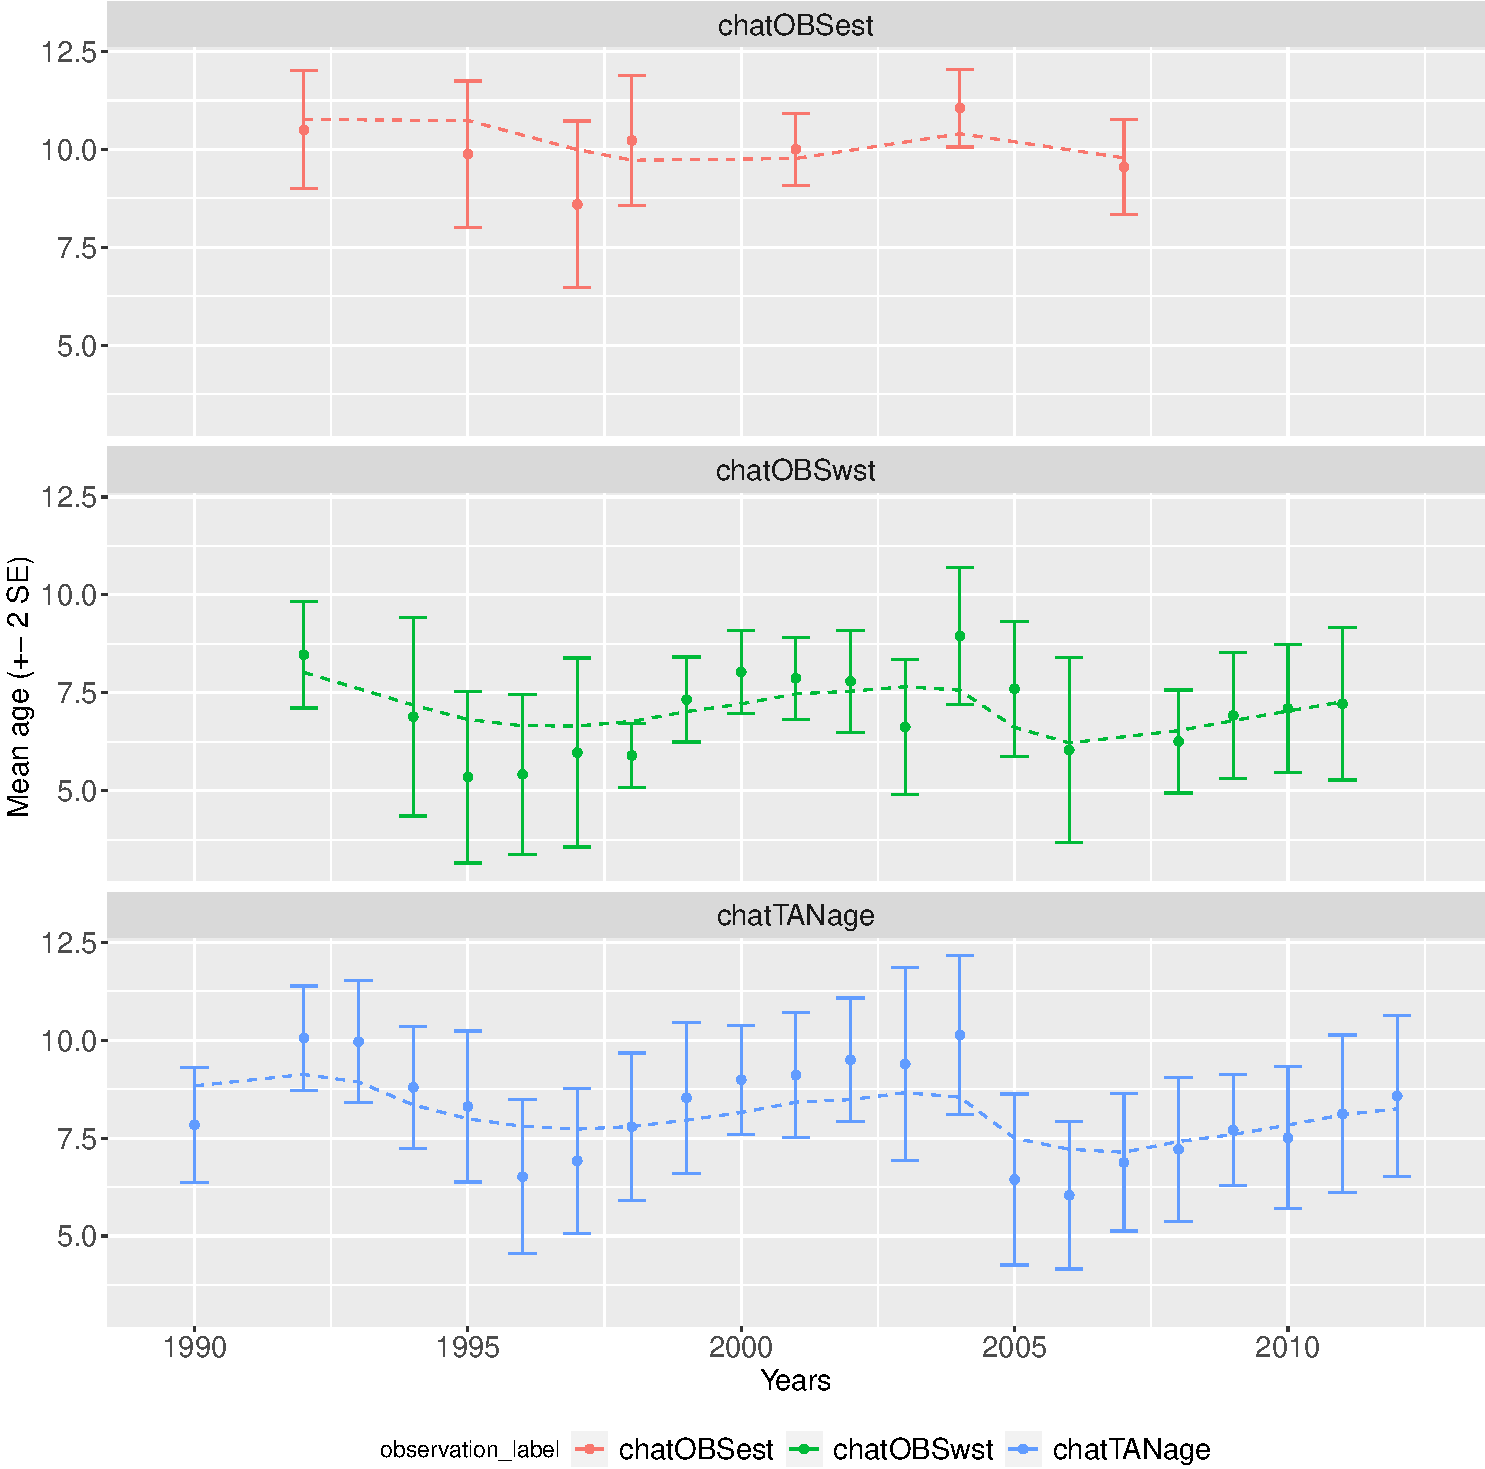
\includegraphics{_main_files/figure-latex/plot_mean_age_fit-1.pdf}

\begin{Shaded}
\begin{Highlighting}[]
\DocumentationTok{\#\# a nice plot with overlapping mean age}
\FunctionTok{ggplot}\NormalTok{(mean\_age\_df, }\FunctionTok{aes}\NormalTok{(}\AttributeTok{x =}\NormalTok{ year, }\AttributeTok{col =}\NormalTok{ observation\_label)) }\SpecialCharTok{+}
  \FunctionTok{geom\_errorbar}\NormalTok{(}\FunctionTok{aes}\NormalTok{(}\AttributeTok{ymin =}\NormalTok{ Oy}\DecValTok{{-}2}\SpecialCharTok{*}\NormalTok{SEy, }\AttributeTok{ymax =}\NormalTok{ Oy }\SpecialCharTok{+} \DecValTok{2}\SpecialCharTok{*}\NormalTok{SEy), }\AttributeTok{width=}\NormalTok{.}\DecValTok{5}\NormalTok{, }
                \AttributeTok{position =} \FunctionTok{position\_dodge}\NormalTok{(}\AttributeTok{width=}\FloatTok{0.9}\NormalTok{)) }\SpecialCharTok{+}
  \FunctionTok{geom\_point}\NormalTok{(}\FunctionTok{aes}\NormalTok{(}\AttributeTok{y =}\NormalTok{ Oy), }\AttributeTok{position =} \FunctionTok{position\_dodge}\NormalTok{(}\AttributeTok{width=}\FloatTok{0.9}\NormalTok{)) }\SpecialCharTok{+}
  \FunctionTok{geom\_line}\NormalTok{(}\FunctionTok{aes}\NormalTok{(}\AttributeTok{y =}\NormalTok{ Ey), }\AttributeTok{linetype =} \StringTok{"dashed"}\NormalTok{) }\SpecialCharTok{+}
  \FunctionTok{labs}\NormalTok{(}\AttributeTok{x =} \StringTok{"Years"}\NormalTok{,}\AttributeTok{y =} \StringTok{"Mean age (+{-} 2 SE)"}\NormalTok{) }\SpecialCharTok{+}
  \FunctionTok{theme\_classic}\NormalTok{() }\SpecialCharTok{+}
  \FunctionTok{theme}\NormalTok{(}\AttributeTok{legend.position =} \StringTok{"right"}\NormalTok{, }
        \AttributeTok{axis.text =} \FunctionTok{element\_text}\NormalTok{(}\AttributeTok{size =} \DecValTok{14}\NormalTok{), }
        \AttributeTok{axis.title =} \FunctionTok{element\_text}\NormalTok{(}\AttributeTok{size =} \DecValTok{14}\NormalTok{),}
        \AttributeTok{strip.text =} \FunctionTok{element\_text}\NormalTok{(}\AttributeTok{size=}\DecValTok{14}\NormalTok{),}
        \AttributeTok{legend.text =} \FunctionTok{element\_text}\NormalTok{(}\AttributeTok{size=}\DecValTok{14}\NormalTok{))}
\end{Highlighting}
\end{Shaded}

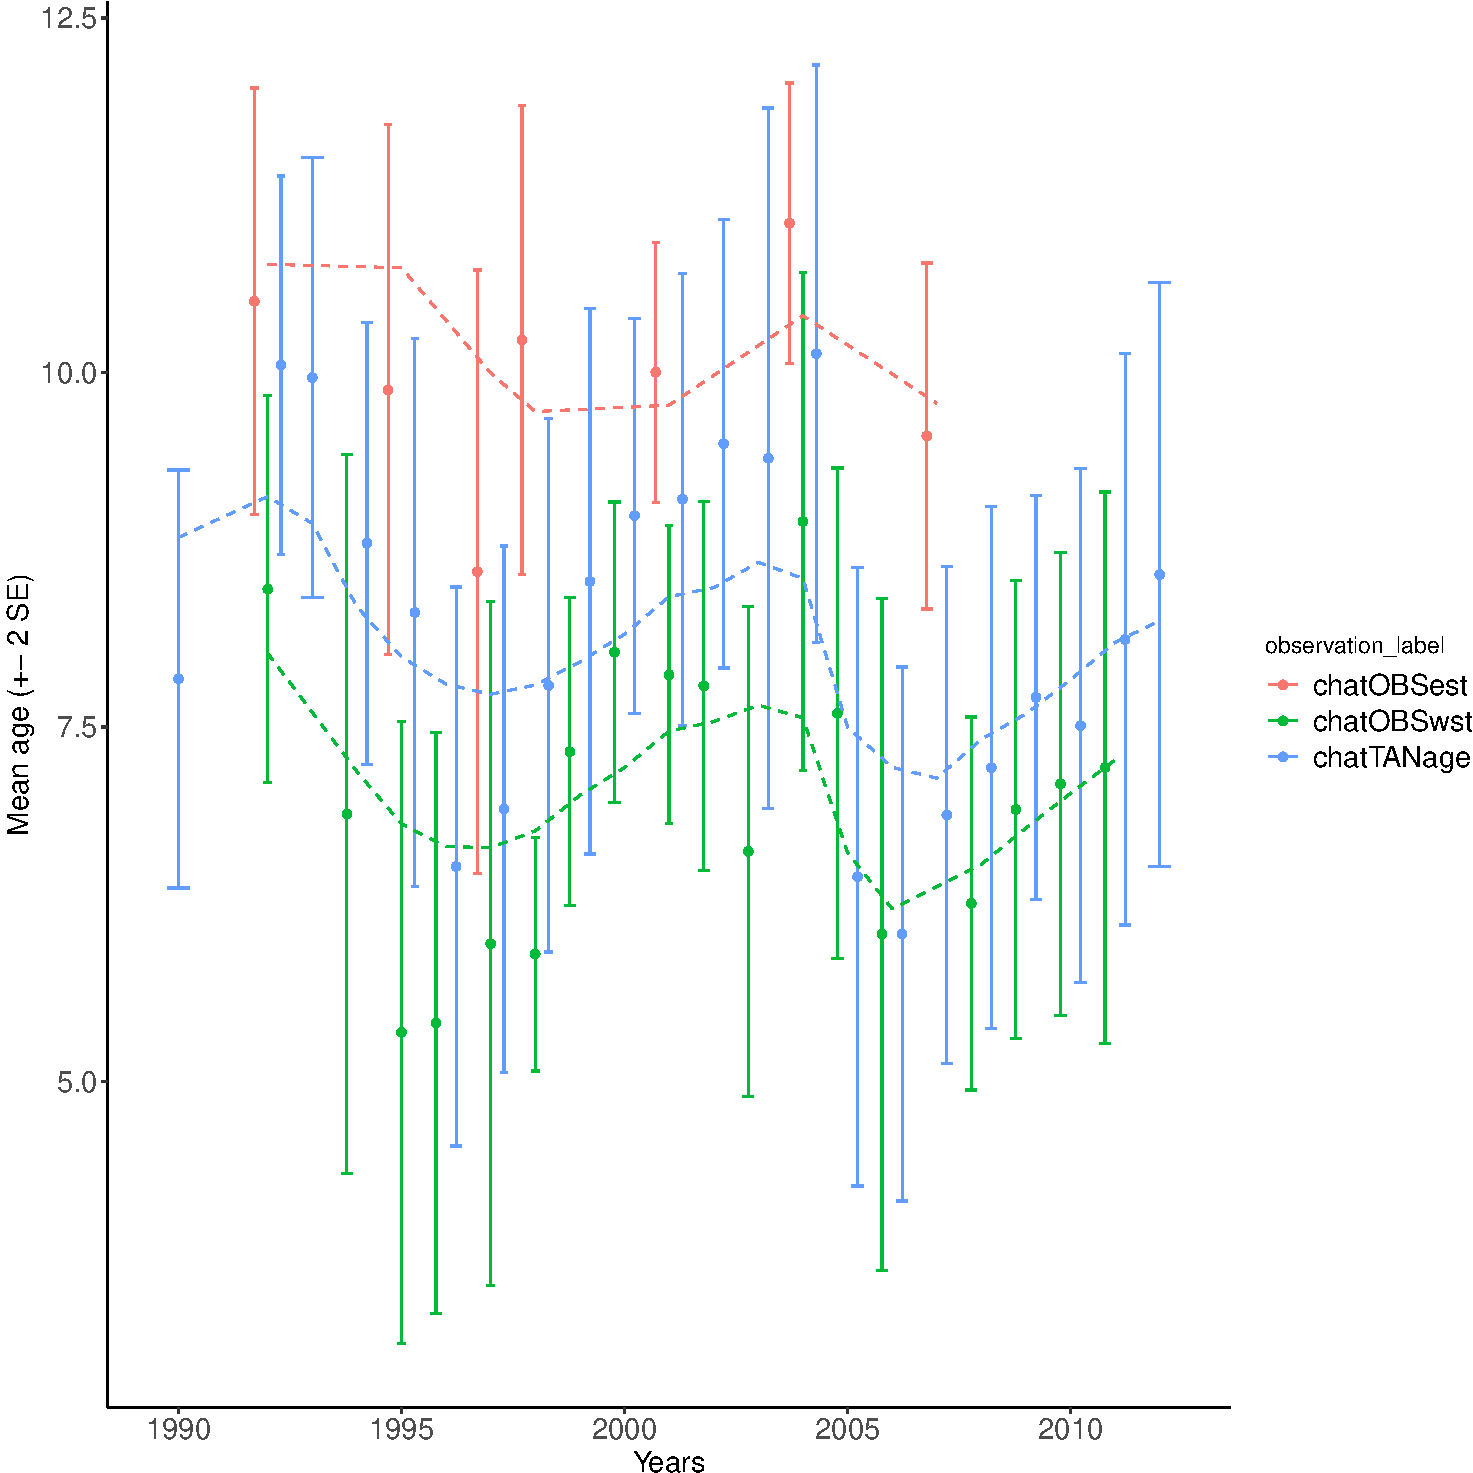
\includegraphics{_main_files/figure-latex/plot_mean_age_fit-2.pdf}

\hypertarget{multiple-casal2-runs-with--i-or--s}{%
\section{Multiple Casal2 runs with -i or -s}\label{multiple-casal2-runs-with--i-or--s}}

\begin{Shaded}
\begin{Highlighting}[]
\NormalTok{file\_name }\OtherTok{=} \FunctionTok{system.file}\NormalTok{(}\StringTok{"extdata"}\NormalTok{, }\StringTok{"SimpleTestModel"}\NormalTok{,}\StringTok{"multi\_run.log"}\NormalTok{, }
                        \AttributeTok{package =} \StringTok{"r4Casal2"}\NormalTok{, }\AttributeTok{mustWork =} \ConstantTok{TRUE}\NormalTok{)}
\NormalTok{mpd }\OtherTok{=} \FunctionTok{extract.mpd}\NormalTok{(}\AttributeTok{file =}\NormalTok{ file\_name)}
\CommentTok{\# Report labels}
\CommentTok{\# names(mpd) }
\CommentTok{\# plot fishing pressures}
\NormalTok{fishery\_df }\OtherTok{=} \FunctionTok{get\_fisheries}\NormalTok{(}\AttributeTok{model =}\NormalTok{ mpd)}
\NormalTok{my\_plot }\OtherTok{=} \FunctionTok{ggplot}\NormalTok{(fishery\_df, }\FunctionTok{aes}\NormalTok{(}\AttributeTok{x =}\NormalTok{ year, }\AttributeTok{y =}\NormalTok{ exploitation, }\AttributeTok{col =} \FunctionTok{factor}\NormalTok{(par\_set))) }\SpecialCharTok{+}
  \FunctionTok{geom\_line}\NormalTok{(}\AttributeTok{size =} \FloatTok{1.4}\NormalTok{) }\SpecialCharTok{+}
  \FunctionTok{facet\_wrap}\NormalTok{(}\SpecialCharTok{\textasciitilde{}}\NormalTok{fishery)}
\NormalTok{my\_plot }\OtherTok{=}\NormalTok{ my\_plot }\SpecialCharTok{+} \FunctionTok{theme}\NormalTok{(}\AttributeTok{axis.text.x =} \FunctionTok{element\_text}\NormalTok{(}\AttributeTok{angle =} \DecValTok{90}\NormalTok{))}
\CommentTok{\# this will generate a generic ggplot}
\FunctionTok{print}\NormalTok{(my\_plot)}
\end{Highlighting}
\end{Shaded}

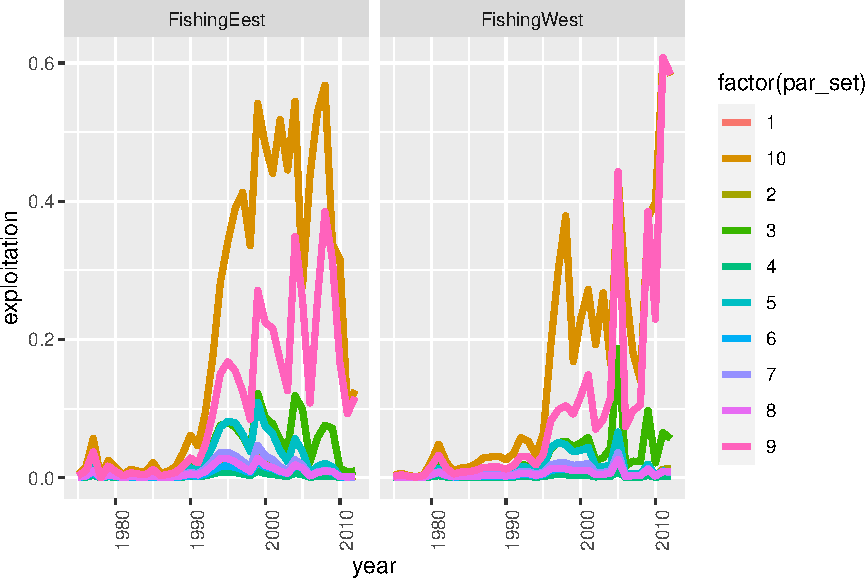
\includegraphics{_main_files/figure-latex/pressures_multi-1.pdf}

\hypertarget{plotting-selectivities-1}{%
\subsection*{Plotting selectivities}\label{plotting-selectivities-1}}
\addcontentsline{toc}{subsection}{Plotting selectivities}

\begin{Shaded}
\begin{Highlighting}[]
\NormalTok{selectivity\_df }\OtherTok{=} \FunctionTok{get\_selectivities}\NormalTok{(mpd)}
\NormalTok{selectivity\_df}\SpecialCharTok{$}\NormalTok{par\_set }\OtherTok{=} \FunctionTok{factor}\NormalTok{(selectivity\_df}\SpecialCharTok{$}\NormalTok{par\_set, }\AttributeTok{ordered =}\NormalTok{ T)}
\FunctionTok{ggplot}\NormalTok{(selectivity\_df, }\FunctionTok{aes}\NormalTok{(}\AttributeTok{x =}\NormalTok{ bin, }\AttributeTok{y =}\NormalTok{ selectivity, }\AttributeTok{col =}\NormalTok{ selectivity\_label, }\AttributeTok{line\_type =}\NormalTok{ par\_set)) }\SpecialCharTok{+}
  \FunctionTok{geom\_line}\NormalTok{(}\AttributeTok{size =} \FloatTok{1.5}\NormalTok{) }\SpecialCharTok{+}
  \FunctionTok{facet\_grid}\NormalTok{(par\_set }\SpecialCharTok{\textasciitilde{}}\NormalTok{ selectivity\_label)}
\end{Highlighting}
\end{Shaded}

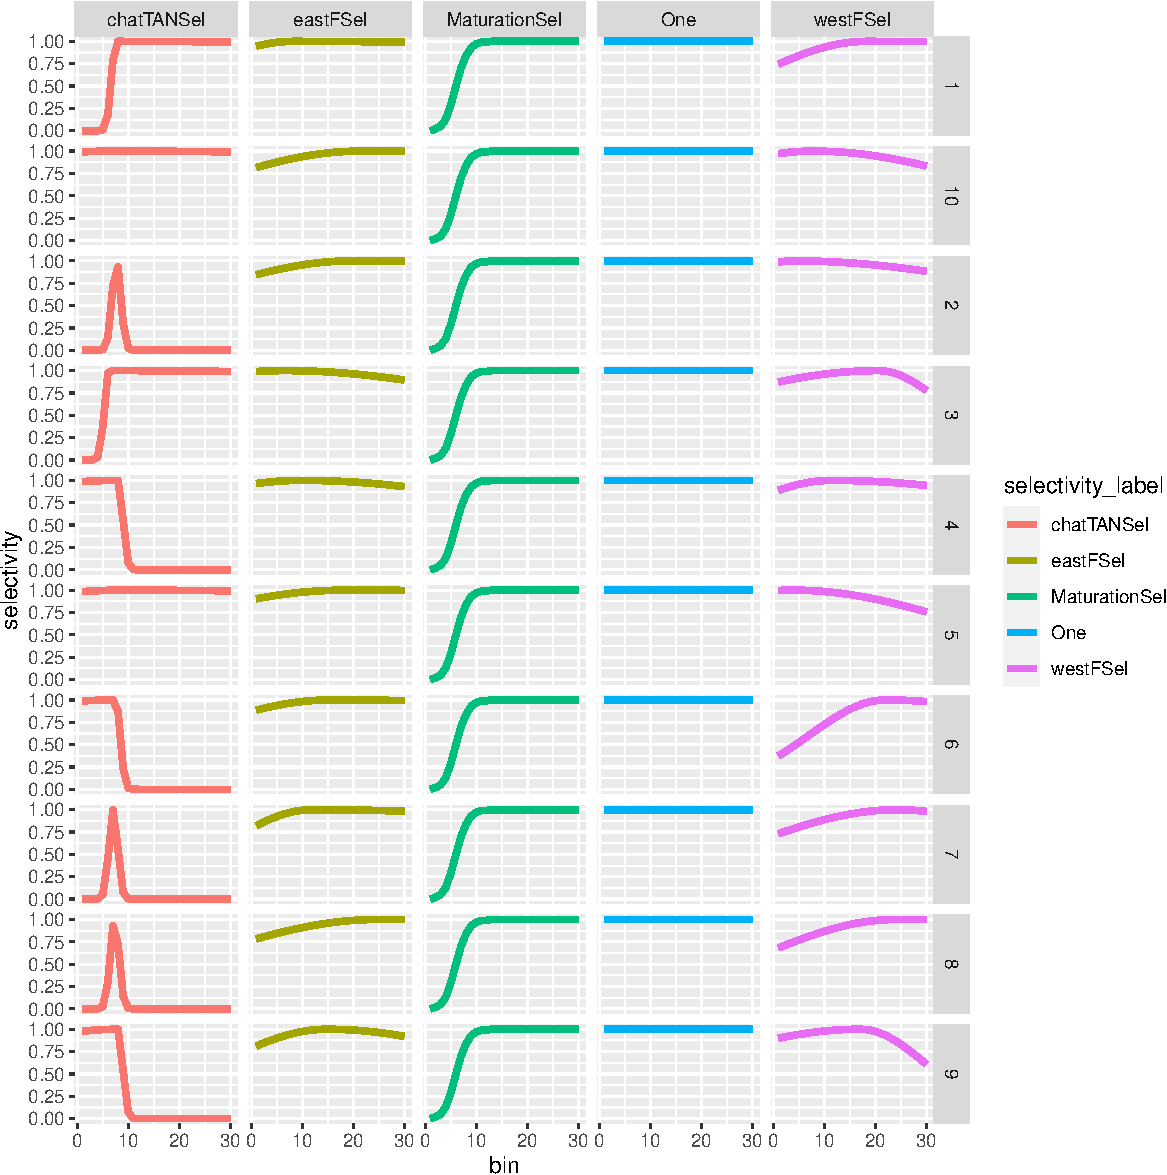
\includegraphics{_main_files/figure-latex/selectivities_multi-1.pdf}

\hypertarget{plotting-fits-1}{%
\subsection*{Plotting Fits}\label{plotting-fits-1}}
\addcontentsline{toc}{subsection}{Plotting Fits}

\begin{Shaded}
\begin{Highlighting}[]
\NormalTok{my\_plot }\OtherTok{=} \FunctionTok{plot\_relative\_index}\NormalTok{(}\AttributeTok{model =}\NormalTok{ mpd, }\AttributeTok{report\_labels =} \FunctionTok{c}\NormalTok{(}\StringTok{"chatTANbiomass"}\NormalTok{), }\AttributeTok{plot.it =}\NormalTok{ T, }\AttributeTok{plot\_type =} \StringTok{"classic"}\NormalTok{)}
\NormalTok{my\_plot}
\end{Highlighting}
\end{Shaded}

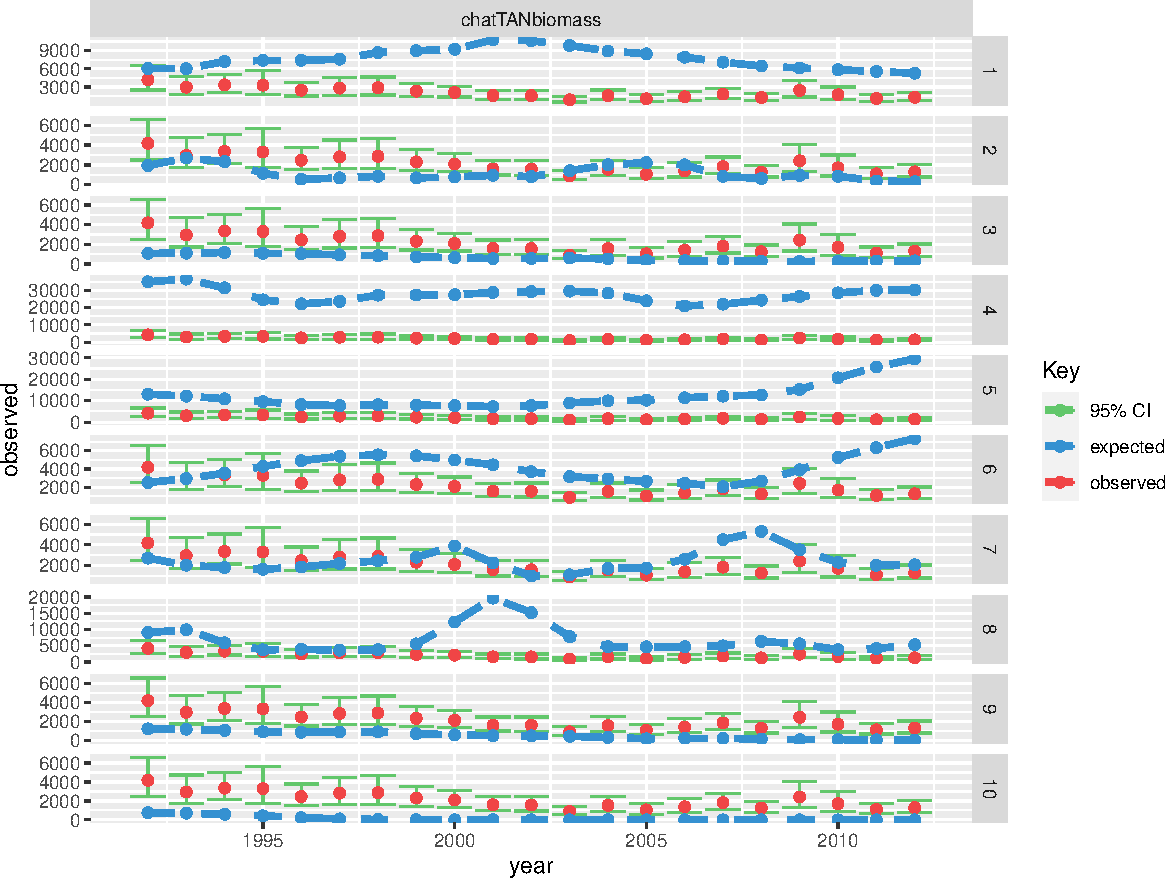
\includegraphics{_main_files/figure-latex/plot_relative_index_multi-1.pdf}

\hypertarget{summarisemultipleinputs}{%
\chapter{Comparing multiple MPD runs}\label{summarisemultipleinputs}}

\hypertarget{read-in-models}{%
\section{Read in models}\label{read-in-models}}

\begin{Shaded}
\begin{Highlighting}[]
\NormalTok{file\_name\_low\_m }\OtherTok{=} \FunctionTok{system.file}\NormalTok{(}\StringTok{"extdata"}\NormalTok{, }\StringTok{"SimpleTestModel"}\NormalTok{ ,}\StringTok{"LowM.log"}\NormalTok{, }
                              \AttributeTok{package =} \StringTok{"r4Casal2"}\NormalTok{, }\AttributeTok{mustWork =} \ConstantTok{TRUE}\NormalTok{)}
\NormalTok{low\_m\_mpd }\OtherTok{=} \FunctionTok{extract.mpd}\NormalTok{(}\AttributeTok{file =}\NormalTok{ file\_name\_low\_m)}
\NormalTok{file\_name\_high\_m }\OtherTok{=} \FunctionTok{system.file}\NormalTok{(}\StringTok{"extdata"}\NormalTok{, }\StringTok{"SimpleTestModel"}\NormalTok{, }\StringTok{"highM.log"}\NormalTok{, }
                               \AttributeTok{package =} \StringTok{"r4Casal2"}\NormalTok{, }\AttributeTok{mustWork =} \ConstantTok{TRUE}\NormalTok{)}
\NormalTok{high\_m\_mpd }\OtherTok{=} \FunctionTok{extract.mpd}\NormalTok{(}\AttributeTok{file =}\NormalTok{ file\_name\_high\_m)}
\DocumentationTok{\#\# create a named list}
\NormalTok{models }\OtherTok{=} \FunctionTok{list}\NormalTok{(}\StringTok{"M = 0.22"} \OtherTok{=}\NormalTok{ low\_m\_mpd, }\StringTok{"M = 0.44"} \OtherTok{=}\NormalTok{ high\_m\_mpd)}
\end{Highlighting}
\end{Shaded}

\hypertarget{compare-model-outputs}{%
\section{Compare model outputs}\label{compare-model-outputs}}

\hypertarget{selectivities}{%
\subsection{selectivities}\label{selectivities}}

\begin{Shaded}
\begin{Highlighting}[]
\NormalTok{selectivity\_df }\OtherTok{=} \FunctionTok{get\_selectivities}\NormalTok{(models)}
\FunctionTok{ggplot}\NormalTok{(selectivity\_df, }\FunctionTok{aes}\NormalTok{(}\AttributeTok{x =}\NormalTok{ bin, }\AttributeTok{y =}\NormalTok{ selectivity, }\AttributeTok{col =}\NormalTok{ model\_label, }\AttributeTok{linetype =}\NormalTok{ model\_label)) }\SpecialCharTok{+}
  \FunctionTok{geom\_line}\NormalTok{(}\AttributeTok{size =} \FloatTok{1.5}\NormalTok{) }\SpecialCharTok{+}
  \FunctionTok{facet\_wrap}\NormalTok{(}\SpecialCharTok{\textasciitilde{}}\NormalTok{selectivity\_label) }\SpecialCharTok{+}
  \FunctionTok{labs}\NormalTok{(}\AttributeTok{x =} \StringTok{"Age"}\NormalTok{, }\AttributeTok{y =} \StringTok{"Ogive"}\NormalTok{, }\AttributeTok{col =} \StringTok{"Model"}\NormalTok{, }\AttributeTok{linetype =} \StringTok{"Model"}\NormalTok{)}
\end{Highlighting}
\end{Shaded}

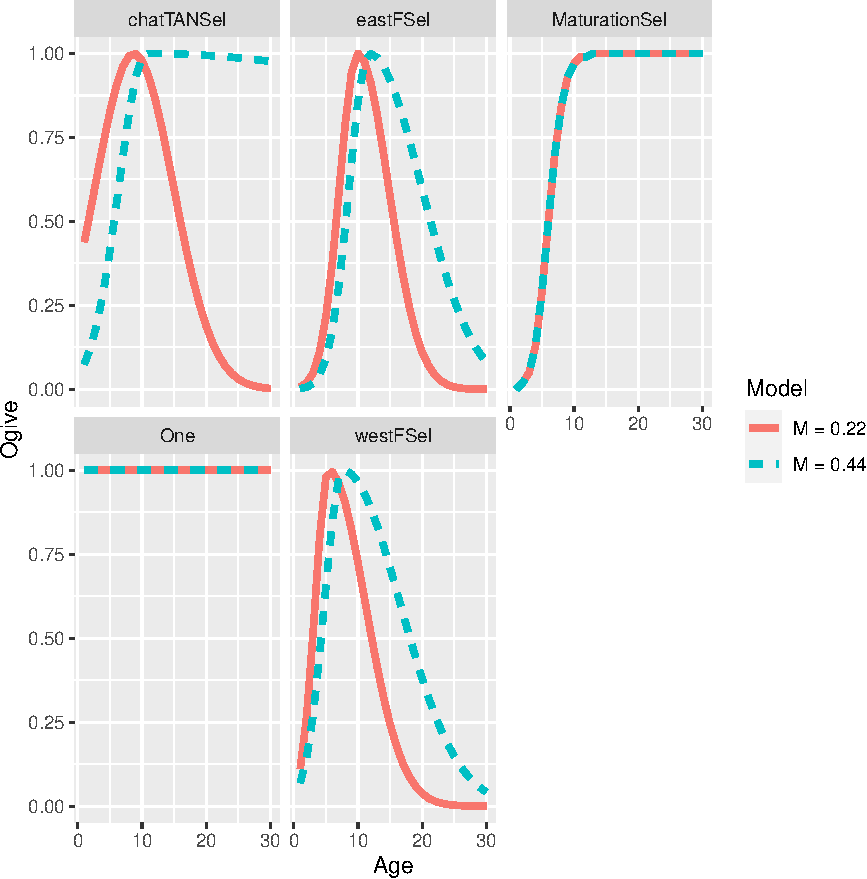
\includegraphics{_main_files/figure-latex/compare_selectivities-1.pdf}

\hypertarget{derived-quantities}{%
\subsection{Derived quantities}\label{derived-quantities}}

\begin{Shaded}
\begin{Highlighting}[]
\NormalTok{dq\_df }\OtherTok{=} \FunctionTok{get\_dqs}\NormalTok{(models)}
\NormalTok{dq\_df}\SpecialCharTok{$}\NormalTok{years }\OtherTok{=} \FunctionTok{as.numeric}\NormalTok{(dq\_df}\SpecialCharTok{$}\NormalTok{years)}
\FunctionTok{ggplot}\NormalTok{(dq\_df, }\FunctionTok{aes}\NormalTok{(}\AttributeTok{x =}\NormalTok{ years, }\AttributeTok{y =}\NormalTok{ values, }\AttributeTok{col =}\NormalTok{ model\_label, }\AttributeTok{linetype =}\NormalTok{ model\_label)) }\SpecialCharTok{+}
  \FunctionTok{geom\_line}\NormalTok{(}\AttributeTok{size =} \FloatTok{1.5}\NormalTok{) }\SpecialCharTok{+}
  \FunctionTok{facet\_wrap}\NormalTok{(}\SpecialCharTok{\textasciitilde{}}\NormalTok{dq\_label) }\SpecialCharTok{+}
  \FunctionTok{labs}\NormalTok{(}\AttributeTok{x =} \StringTok{"Year"}\NormalTok{, }\AttributeTok{y =} \StringTok{"SSB"}\NormalTok{, }\AttributeTok{col =} \StringTok{"Model"}\NormalTok{, }\AttributeTok{linetype =} \StringTok{"Model"}\NormalTok{)}
\end{Highlighting}
\end{Shaded}

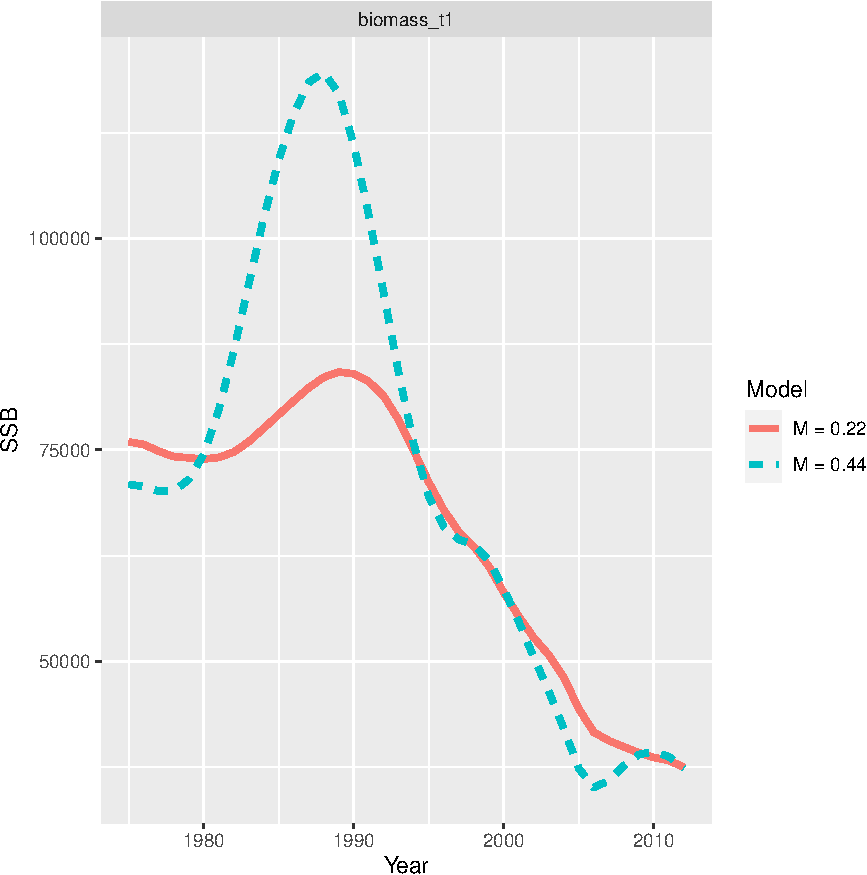
\includegraphics{_main_files/figure-latex/compare_dqs-1.pdf}

\hypertarget{recruitment}{%
\subsection{Recruitment}\label{recruitment}}

\begin{Shaded}
\begin{Highlighting}[]
\NormalTok{recruit\_df }\OtherTok{=} \FunctionTok{get\_BH\_recruitment}\NormalTok{(models)}
\FunctionTok{ggplot}\NormalTok{(recruit\_df, }\FunctionTok{aes}\NormalTok{(}\AttributeTok{x =}\NormalTok{ model\_year, }\AttributeTok{y =}\NormalTok{ standardised\_recruitment\_multipliers, }\AttributeTok{col =}\NormalTok{ model\_label, }\AttributeTok{linetype =}\NormalTok{ model\_label)) }\SpecialCharTok{+}
  \FunctionTok{geom\_line}\NormalTok{(}\AttributeTok{size =} \FloatTok{1.3}\NormalTok{) }\SpecialCharTok{+}
  \FunctionTok{labs}\NormalTok{(}\AttributeTok{x =} \StringTok{"Recruited year"}\NormalTok{, }\AttributeTok{y =} \StringTok{"standardised recruitment multipliers"}\NormalTok{, }\AttributeTok{col =} \StringTok{"Model"}\NormalTok{, }\AttributeTok{linetype =} \StringTok{"Model"}\NormalTok{)}
\end{Highlighting}
\end{Shaded}

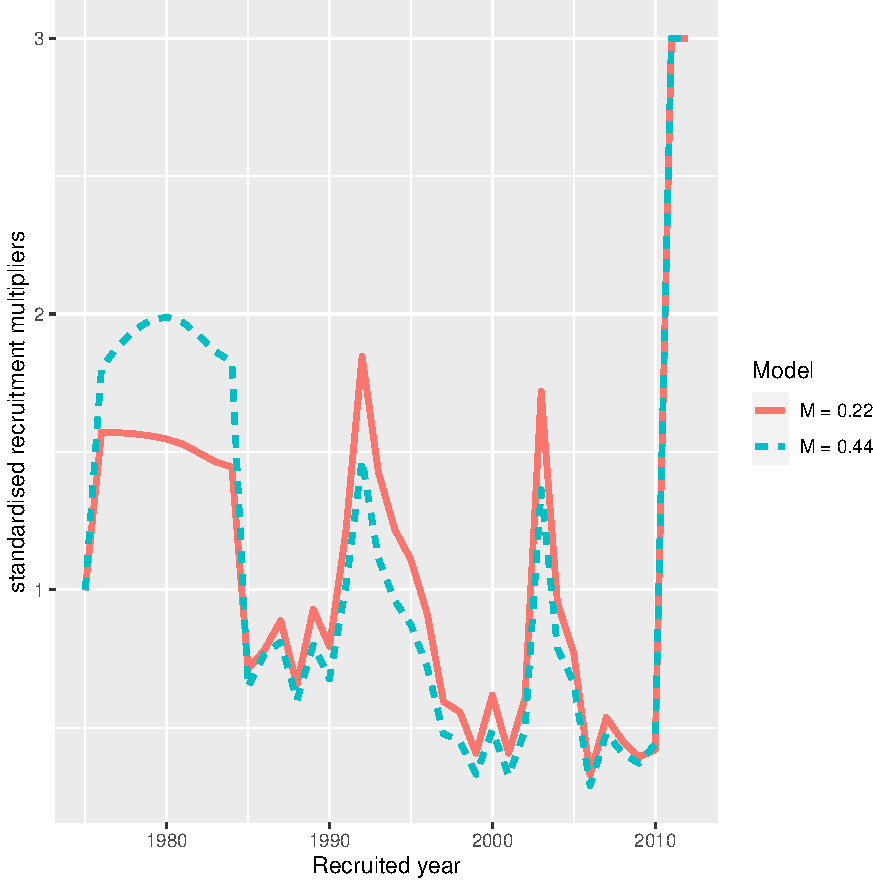
\includegraphics{_main_files/figure-latex/compare_recruit-1.pdf}

\hypertarget{abundance-fits}{%
\subsection{Abundance fits}\label{abundance-fits}}

\begin{Shaded}
\begin{Highlighting}[]
\NormalTok{abundance\_obs\_df }\OtherTok{=} \FunctionTok{get\_abundance\_observations}\NormalTok{(models)}
\FunctionTok{ggplot}\NormalTok{(abundance\_obs\_df, }\FunctionTok{aes}\NormalTok{(}\AttributeTok{x =}\NormalTok{ year)) }\SpecialCharTok{+}
  \FunctionTok{geom\_point}\NormalTok{(}\FunctionTok{aes}\NormalTok{(}\AttributeTok{y =}\NormalTok{ observed), }\AttributeTok{size =} \FloatTok{1.4}\NormalTok{) }\SpecialCharTok{+}
  \FunctionTok{geom\_line}\NormalTok{(}\FunctionTok{aes}\NormalTok{(}\AttributeTok{y =}\NormalTok{ expected, }\AttributeTok{col =}\NormalTok{ model\_label)) }\SpecialCharTok{+}
  \FunctionTok{labs}\NormalTok{(}\AttributeTok{x =} \StringTok{"year"}\NormalTok{, }\AttributeTok{y =} \StringTok{"Abundance"}\NormalTok{, }\AttributeTok{col =} \StringTok{"Model"}\NormalTok{, }\AttributeTok{linetype =} \StringTok{"Model"}\NormalTok{) }\SpecialCharTok{+}
  \FunctionTok{facet\_wrap}\NormalTok{(}\SpecialCharTok{\textasciitilde{}}\NormalTok{observation\_label, }\AttributeTok{scales =} \StringTok{"free"}\NormalTok{)}
\end{Highlighting}
\end{Shaded}

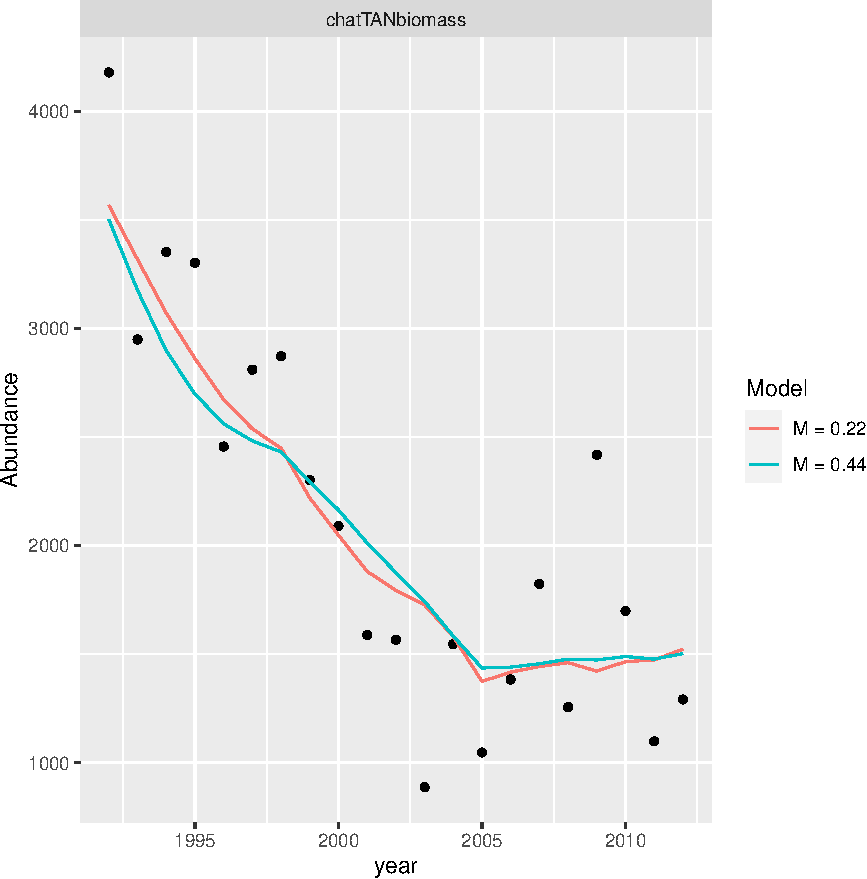
\includegraphics{_main_files/figure-latex/compare_abundance-1.pdf}

\hypertarget{compare-objective-function}{%
\subsection{Compare objective function}\label{compare-objective-function}}

\begin{Shaded}
\begin{Highlighting}[]
\NormalTok{cas2\_obj }\OtherTok{=} \FunctionTok{get\_objective\_function}\NormalTok{(models)}
\NormalTok{compar\_obj }\OtherTok{=}\NormalTok{ cas2\_obj }\SpecialCharTok{\%\textgreater{}\%} \FunctionTok{pivot\_wider}\NormalTok{(}\AttributeTok{values\_from =}\NormalTok{ negative\_loglik, }\AttributeTok{names\_from =}\NormalTok{ model\_label, }\AttributeTok{id\_cols =}\NormalTok{ component, }\AttributeTok{values\_fill =} \ConstantTok{NA}\NormalTok{)}
\FunctionTok{head}\NormalTok{(compar\_obj, }\AttributeTok{n =} \DecValTok{10}\NormalTok{)}
\end{Highlighting}
\end{Shaded}

\begin{verbatim}
## # A tibble: 10 x 3
##    component                   `M = 0.22`  `M = 0.44`
##    <chr>                            <dbl>       <dbl>
##  1 observation-chatTANbiomass -20.2       -19.7      
##  2 observation-chatTANage     339.        346.       
##  3 observation-chatOBSwst     227.        227.       
##  4 observation-chatOBSest     127.        127.       
##  5 penalty-CatchMustBeTaken1    0           0        
##  6 prior-B0                    11.2        11.2      
##  7 prior-chatTANq              -2.32       -1.80     
##  8 prior-TANSel_mu              0.256       3.50     
##  9 prior-TANSel_sig_l           0.0000171   0.0000502
## 10 prior-TANSel_sig_r           0.0000148   0.0177
\end{verbatim}

\begin{Shaded}
\begin{Highlighting}[]
\DocumentationTok{\#\# rescale objective score so the model with the best fit (lowest score)}
\DocumentationTok{\#\# will have zero for a given component and others will have be reference from that}
\NormalTok{obj\_df }\OtherTok{=}\NormalTok{ cas2\_obj }\SpecialCharTok{\%\textgreater{}\%} \FunctionTok{group\_by}\NormalTok{(component) }\SpecialCharTok{\%\textgreater{}\%} 
  \FunctionTok{mutate}\NormalTok{(}\AttributeTok{rescaled\_obj =}\NormalTok{ negative\_loglik }\SpecialCharTok{{-}} \FunctionTok{min}\NormalTok{(negative\_loglik, }\AttributeTok{na.rm =}\NormalTok{ T))}
\DocumentationTok{\#\# plot it for each component}
\FunctionTok{ggplot}\NormalTok{(obj\_df, }\FunctionTok{aes}\NormalTok{(}\AttributeTok{x =}\NormalTok{ rescaled\_obj, }\AttributeTok{y =}\NormalTok{ component, }\AttributeTok{col =}\NormalTok{ model\_label, }\AttributeTok{shape =}\NormalTok{ model\_label)) }\SpecialCharTok{+}
  \FunctionTok{geom\_point}\NormalTok{(}\AttributeTok{size =} \DecValTok{2}\NormalTok{) }\SpecialCharTok{+}
  \FunctionTok{labs}\NormalTok{(}\AttributeTok{x =} \StringTok{"Objective function {-} min (objective function)"}\NormalTok{, }\AttributeTok{y =} \StringTok{""}\NormalTok{) }\SpecialCharTok{+}
  \FunctionTok{geom\_vline}\NormalTok{(}\AttributeTok{xintercept =} \DecValTok{0}\NormalTok{, }\AttributeTok{col =} \StringTok{"gray"}\NormalTok{, }\AttributeTok{linetype =} \StringTok{"dashed"}\NormalTok{, }\AttributeTok{size =} \DecValTok{1}\NormalTok{) }\SpecialCharTok{+}
  \FunctionTok{theme}\NormalTok{(}\AttributeTok{legend.position =} \StringTok{"bottom"}\NormalTok{, }
        \AttributeTok{axis.text =} \FunctionTok{element\_text}\NormalTok{(}\AttributeTok{size =} \DecValTok{12}\NormalTok{), }
        \AttributeTok{axis.title =} \FunctionTok{element\_text}\NormalTok{(}\AttributeTok{size =} \DecValTok{12}\NormalTok{),}
        \AttributeTok{strip.text =} \FunctionTok{element\_text}\NormalTok{(}\AttributeTok{size=}\DecValTok{16}\NormalTok{),}
        \AttributeTok{title=}\FunctionTok{element\_blank}\NormalTok{(),}
        \AttributeTok{legend.text =} \FunctionTok{element\_text}\NormalTok{(}\AttributeTok{size=}\DecValTok{14}\NormalTok{))}
\end{Highlighting}
\end{Shaded}

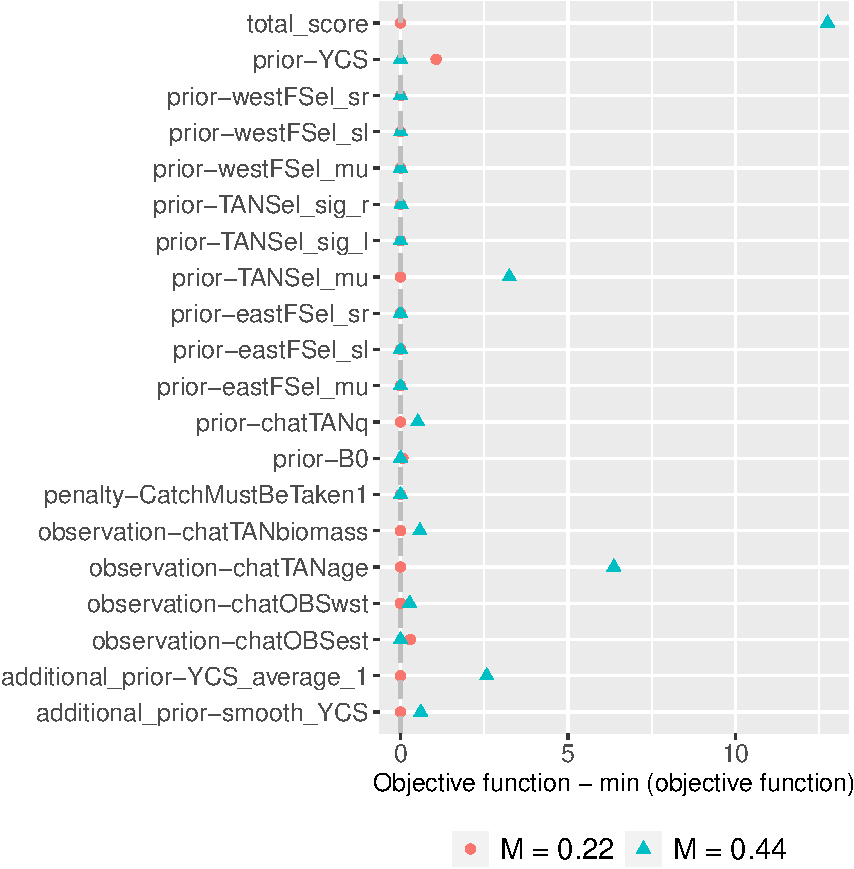
\includegraphics{_main_files/figure-latex/obj_plot-1.pdf}

\hypertarget{mcmc}{%
\chapter{MCMC}\label{mcmc}}

Casal2 MCMC estimation for a single model should be done using ``multiple chains''. A chain in this case is a separate MCMC run, ideally starting from a different set of starting locations and with a different seed number. It is advised to create at least three chains per model. Most of the MCMC diagnostics in this package are designed for multiple chains. These include calculating Rhats (within and between chain variation in parameters) \citep{vehtari2021rank} and effective sample sizes which is a measure of efficiency in your mcmc sampler.

\hypertarget{read-in-models-1}{%
\section{Read in models}\label{read-in-models-1}}

\begin{Shaded}
\begin{Highlighting}[]
\DocumentationTok{\#\# extra packages}
\FunctionTok{library}\NormalTok{(purrr)}
\FunctionTok{library}\NormalTok{(bayesplot)}

\NormalTok{cas2\_file\_dir }\OtherTok{=} \FunctionTok{system.file}\NormalTok{(}\StringTok{"extdata"}\NormalTok{, }\StringTok{"multi\_chain\_mcmc"}\NormalTok{, }\AttributeTok{package =} \StringTok{"r4Casal2"}\NormalTok{, }\AttributeTok{mustWork =} \ConstantTok{TRUE}\NormalTok{)}
\NormalTok{mcmc\_1 }\OtherTok{=} \FunctionTok{extract.mcmc}\NormalTok{(}\AttributeTok{path =}\NormalTok{ cas2\_file\_dir, }\AttributeTok{samples.file =} \StringTok{"samples.4"}\NormalTok{, }\AttributeTok{objectives.file =} \StringTok{"objectives.4"}\NormalTok{)}
\NormalTok{mcmc\_2 }\OtherTok{=} \FunctionTok{extract.mcmc}\NormalTok{(}\AttributeTok{path =}\NormalTok{ cas2\_file\_dir, }\AttributeTok{samples.file =} \StringTok{"samples.5"}\NormalTok{, }\AttributeTok{objectives.file =} \StringTok{"objectives.5"}\NormalTok{)}
\NormalTok{mcmc\_3 }\OtherTok{=} \FunctionTok{extract.mcmc}\NormalTok{(}\AttributeTok{path =}\NormalTok{ cas2\_file\_dir, }\AttributeTok{samples.file =} \StringTok{"samples.6"}\NormalTok{, }\AttributeTok{objectives.file =} \StringTok{"objectives.6"}\NormalTok{)}
\DocumentationTok{\#\# assign chain label}
\NormalTok{mcmc\_1}\SpecialCharTok{$}\NormalTok{chain }\OtherTok{=} \StringTok{"1"}
\NormalTok{mcmc\_2}\SpecialCharTok{$}\NormalTok{chain }\OtherTok{=} \StringTok{"2"}
\NormalTok{mcmc\_3}\SpecialCharTok{$}\NormalTok{chain }\OtherTok{=} \StringTok{"3"}
\DocumentationTok{\#\# Remove burn{-}in iterations}
\NormalTok{mcmc\_post\_1 }\OtherTok{=}\NormalTok{ mcmc\_1 }\SpecialCharTok{\%\textgreater{}\%} \FunctionTok{filter}\NormalTok{(state }\SpecialCharTok{==} \StringTok{"mcmc"}\NormalTok{)}
\NormalTok{mcmc\_post\_2 }\OtherTok{=}\NormalTok{ mcmc\_2 }\SpecialCharTok{\%\textgreater{}\%} \FunctionTok{filter}\NormalTok{(state }\SpecialCharTok{==} \StringTok{"mcmc"}\NormalTok{)}
\NormalTok{mcmc\_post\_3 }\OtherTok{=}\NormalTok{ mcmc\_3 }\SpecialCharTok{\%\textgreater{}\%} \FunctionTok{filter}\NormalTok{(state }\SpecialCharTok{==} \StringTok{"mcmc"}\NormalTok{)}
\DocumentationTok{\#\# combine}
\NormalTok{mcmc\_all }\OtherTok{=} \FunctionTok{rbind}\NormalTok{(mcmc\_1, mcmc\_2, mcmc\_3)}
\NormalTok{mcmc\_non\_burn\_in }\OtherTok{=}\NormalTok{ mcmc\_all }\SpecialCharTok{\%\textgreater{}\%} \FunctionTok{filter}\NormalTok{(state }\SpecialCharTok{==} \StringTok{"mcmc"}\NormalTok{)}
\NormalTok{n\_posterior\_samples }\OtherTok{=}  \FunctionTok{nrow}\NormalTok{(mcmc\_post\_1) }\SpecialCharTok{+} \FunctionTok{nrow}\NormalTok{(mcmc\_post\_2) }\SpecialCharTok{+} \FunctionTok{nrow}\NormalTok{(mcmc\_post\_3)}
\DocumentationTok{\#\# do some modifying so we have just parameters available}
\DocumentationTok{\#\# }\AlertTok{TODO}\DocumentationTok{: change parameter labels so they are not so large and easier to read on figures}
\NormalTok{pars }\OtherTok{=} \FunctionTok{colnames}\NormalTok{(mcmc\_post\_1[,}\DecValTok{12}\SpecialCharTok{:}\NormalTok{(}\FunctionTok{ncol}\NormalTok{(mcmc\_non\_burn\_in) }\SpecialCharTok{{-}} \DecValTok{1}\NormalTok{)])}
\NormalTok{iters }\OtherTok{=} \FunctionTok{max}\NormalTok{(}\FunctionTok{nrow}\NormalTok{(mcmc\_post\_1), }\FunctionTok{nrow}\NormalTok{(mcmc\_post\_2), }\FunctionTok{nrow}\NormalTok{(mcmc\_post\_3))}
\NormalTok{bayes\_array }\OtherTok{=} \FunctionTok{array}\NormalTok{(}\AttributeTok{dim =} \FunctionTok{c}\NormalTok{(iters, }\DecValTok{3}\NormalTok{, }\FunctionTok{length}\NormalTok{(pars)), }\AttributeTok{dimnames =} \FunctionTok{list}\NormalTok{(}\DecValTok{1}\SpecialCharTok{:}\NormalTok{iters, }\DecValTok{1}\SpecialCharTok{:}\DecValTok{3}\NormalTok{, pars))}
\NormalTok{bayes\_array[}\DecValTok{1}\SpecialCharTok{:}\FunctionTok{nrow}\NormalTok{(mcmc\_post\_1),}\DecValTok{1}\NormalTok{,] }\OtherTok{=} \FunctionTok{as.matrix}\NormalTok{(mcmc\_post\_1[,}\DecValTok{12}\SpecialCharTok{:}\NormalTok{(}\FunctionTok{ncol}\NormalTok{(mcmc\_non\_burn\_in) }\SpecialCharTok{{-}} \DecValTok{1}\NormalTok{)])}
\NormalTok{bayes\_array[}\DecValTok{1}\SpecialCharTok{:}\FunctionTok{nrow}\NormalTok{(mcmc\_post\_2),}\DecValTok{2}\NormalTok{,] }\OtherTok{=} \FunctionTok{as.matrix}\NormalTok{(mcmc\_post\_2[,}\DecValTok{12}\SpecialCharTok{:}\NormalTok{(}\FunctionTok{ncol}\NormalTok{(mcmc\_non\_burn\_in) }\SpecialCharTok{{-}} \DecValTok{1}\NormalTok{)])}
\NormalTok{bayes\_array[}\DecValTok{1}\SpecialCharTok{:}\FunctionTok{nrow}\NormalTok{(mcmc\_post\_3),}\DecValTok{3}\NormalTok{,] }\OtherTok{=} \FunctionTok{as.matrix}\NormalTok{(mcmc\_post\_3[,}\DecValTok{12}\SpecialCharTok{:}\NormalTok{(}\FunctionTok{ncol}\NormalTok{(mcmc\_non\_burn\_in) }\SpecialCharTok{{-}} \DecValTok{1}\NormalTok{)])}
\DocumentationTok{\#\# cut off at min}
\NormalTok{min\_cutoff }\OtherTok{=} \FunctionTok{min}\NormalTok{(}\FunctionTok{nrow}\NormalTok{(mcmc\_post\_1), }\FunctionTok{nrow}\NormalTok{(mcmc\_post\_2), }\FunctionTok{nrow}\NormalTok{(mcmc\_post\_3))}
\NormalTok{bayes\_array }\OtherTok{=}\NormalTok{ bayes\_array[}\DecValTok{1}\SpecialCharTok{:}\NormalTok{min\_cutoff, ,]}
\end{Highlighting}
\end{Shaded}

\hypertarget{diagnostics}{%
\section{Diagnostics}\label{diagnostics}}

\begin{Shaded}
\begin{Highlighting}[]
\DocumentationTok{\#\# get Rhats}
\NormalTok{rhats }\OtherTok{=} \FunctionTok{apply}\NormalTok{(bayes\_array, }\AttributeTok{MARGIN =} \DecValTok{3}\NormalTok{, Rhat)}
\DocumentationTok{\#\# get effective sample sizes}
\NormalTok{n\_eff\_bulk }\OtherTok{=} \FunctionTok{apply}\NormalTok{(bayes\_array, }\AttributeTok{MARGIN =} \DecValTok{3}\NormalTok{, ess\_bulk)}
\NormalTok{n\_eff\_tail }\OtherTok{=} \FunctionTok{apply}\NormalTok{(bayes\_array, }\AttributeTok{MARGIN =} \DecValTok{3}\NormalTok{, ess\_tail)}
\DocumentationTok{\#\# }\AlertTok{TODO}\DocumentationTok{: need to think about what is a good general rule of thumb. }
\DocumentationTok{\#\# I was thinking you would want n\_eff of at least 200.}
\end{Highlighting}
\end{Shaded}

The \texttt{Rhat} function produces R-hat convergence diagnostic, which compares the between- and within-chain estimates for model parameters and other univariate quantities of interest. Chains that have not mixed well (i.e., the between-and within-chain estimates don't agree) will result in R-hat larger than 1.1. The \texttt{ess\_bulk} function produces an estimated Bulk Effective Sample Size (bulk-ESS) using rank normalized draws. Bulk-ESS is useful measure for sampling efficiency in the bulk of the distribution (related e.g.~to efficiency of mean and median estimates), and is well defined even if the chains do not have finite mean or variance. The \texttt{ess\_tail} function produces an estimated Tail Effective Sample Size (tail-ESS) by computing the minimum of effective sample sizes for 5\% and 95\% quantiles. Tail-ESS is useful measure for sampling efficiency in the tails of the distribution (related e.g.~to efficiency of variance and tail quantile estimates).

Once you have calculated these quantities you can use \texttt{bayesplot} plotting functions. Need to work on changing parameter labels from the Casal2 model. They make some of these plots difficult to read

\begin{Shaded}
\begin{Highlighting}[]
\FunctionTok{mcmc\_rhat}\NormalTok{(rhats)}
\end{Highlighting}
\end{Shaded}

\begin{verbatim}
## Warning: Dropped 6 NAs from 'new_rhat(rhat)'.
\end{verbatim}

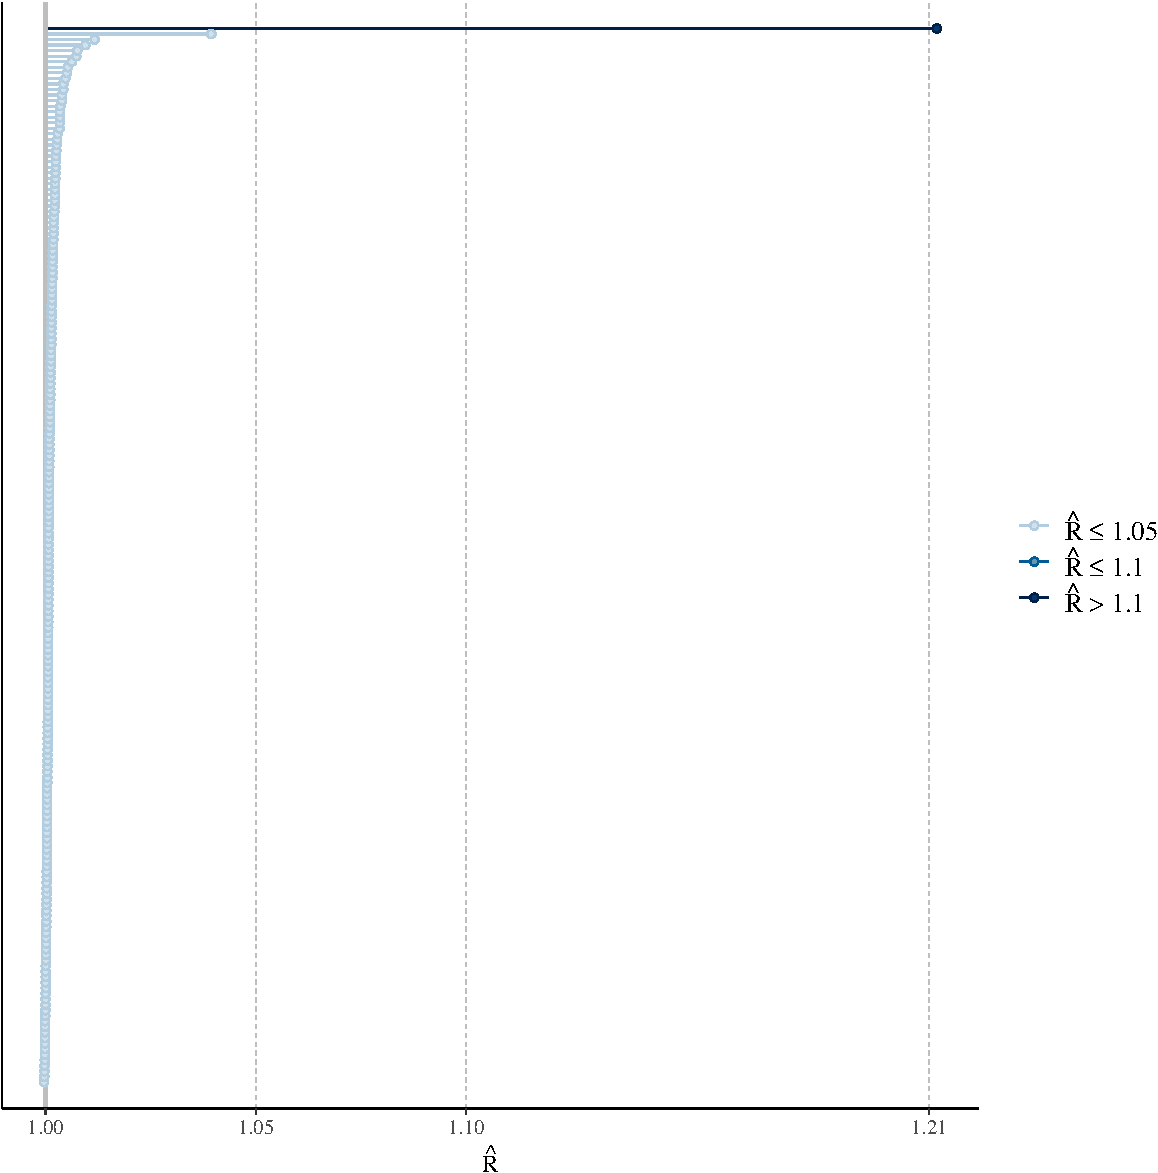
\includegraphics{_main_files/figure-latex/plot_rhats-1.pdf}

\begin{Shaded}
\begin{Highlighting}[]
\CommentTok{\#mcmc\_neff(n\_eff\_bulk)}
\CommentTok{\#mcmc\_neff(n\_eff\_tail)}
\end{Highlighting}
\end{Shaded}

\hypertarget{plotting-quantities}{%
\section{Plotting quantities}\label{plotting-quantities}}

\begin{Shaded}
\begin{Highlighting}[]
\DocumentationTok{\#\# This function helps create 95\% CIs for quantities}
\NormalTok{p }\OtherTok{\textless{}{-}} \FunctionTok{c}\NormalTok{(}\FloatTok{0.025}\NormalTok{, }\FloatTok{0.5}\NormalTok{, }\FloatTok{0.975}\NormalTok{) }\DocumentationTok{\#\# confidence intervals}
\NormalTok{p\_names }\OtherTok{\textless{}{-}} \FunctionTok{map\_chr}\NormalTok{(p, }\SpecialCharTok{\textasciitilde{}}\FunctionTok{paste0}\NormalTok{(.x}\SpecialCharTok{*}\DecValTok{100}\NormalTok{, }\StringTok{"\%"}\NormalTok{))}
\NormalTok{p\_funs }\OtherTok{\textless{}{-}} \FunctionTok{map}\NormalTok{(p, }\SpecialCharTok{\textasciitilde{}}\FunctionTok{partial}\NormalTok{(quantile, }\AttributeTok{probs =}\NormalTok{ .x, }\AttributeTok{na.rm =} \ConstantTok{TRUE}\NormalTok{)) }\SpecialCharTok{\%\textgreater{}\%} 
\NormalTok{  rlang}\SpecialCharTok{::}\FunctionTok{set\_names}\NormalTok{(}\AttributeTok{nm =} \FunctionTok{c}\NormalTok{(}\StringTok{"low"}\NormalTok{, }\StringTok{"mid"}\NormalTok{, }\StringTok{"upp"}\NormalTok{))}
\CommentTok{\#p\_funs}

\DocumentationTok{\#\# Bring in derived quantities}
\NormalTok{cas2\_file\_name }\OtherTok{=} \FunctionTok{system.file}\NormalTok{(}\StringTok{"extdata"}\NormalTok{, }\StringTok{"tabular.log"}\NormalTok{, }\AttributeTok{package =} \StringTok{"r4Casal2"}\NormalTok{, }\AttributeTok{mustWork =} \ConstantTok{TRUE}\NormalTok{)}
\NormalTok{cas2\_tab }\OtherTok{=} \FunctionTok{extract.tabular}\NormalTok{(}\AttributeTok{file =}\NormalTok{ cas2\_file\_name, }\AttributeTok{quiet =}\NormalTok{ T)}
\DocumentationTok{\#\# cut off burn{-}in the first 50 samples}
\NormalTok{cas2\_tab }\OtherTok{=} \FunctionTok{burn.in.tabular}\NormalTok{(cas2\_tab, }\AttributeTok{Row =} \DecValTok{50}\NormalTok{)}
\end{Highlighting}
\end{Shaded}

\hypertarget{selectivities-1}{%
\subsection{selectivities}\label{selectivities-1}}

\begin{Shaded}
\begin{Highlighting}[]
\NormalTok{selectivity\_df }\OtherTok{=} \FunctionTok{get\_selectivities}\NormalTok{(cas2\_tab)}
\NormalTok{quantile\_selectivity\_df }\OtherTok{=}\NormalTok{ selectivity\_df }\SpecialCharTok{\%\textgreater{}\%} 
  \FunctionTok{group\_by}\NormalTok{(bin, selectivity\_label) }\SpecialCharTok{\%\textgreater{}\%} 
  \FunctionTok{summarize\_at}\NormalTok{(}\FunctionTok{vars}\NormalTok{(selectivity), p\_funs)}

\FunctionTok{ggplot}\NormalTok{(quantile\_selectivity\_df, }\FunctionTok{aes}\NormalTok{(}\AttributeTok{x =}\NormalTok{ bin)) }\SpecialCharTok{+}
  \FunctionTok{geom\_ribbon}\NormalTok{(}\FunctionTok{aes}\NormalTok{(}\AttributeTok{ymax  =}\NormalTok{ low, }\AttributeTok{ymin =}\NormalTok{ upp, }\AttributeTok{alpha =} \FloatTok{0.5}\NormalTok{, }\AttributeTok{col =}\NormalTok{ selectivity\_label, }\AttributeTok{fill =}\NormalTok{ selectivity\_label), }\AttributeTok{lwd=}\DecValTok{0}\NormalTok{) }\SpecialCharTok{+}
  \FunctionTok{geom\_line}\NormalTok{(}\FunctionTok{aes}\NormalTok{(}\AttributeTok{y =}\NormalTok{ mid, }\AttributeTok{col =}\NormalTok{ selectivity\_label, }\AttributeTok{group =}\NormalTok{ selectivity\_label), }\AttributeTok{size =}\DecValTok{2}\NormalTok{, }\AttributeTok{alpha =} \DecValTok{1}\NormalTok{) }\SpecialCharTok{+}
  \FunctionTok{facet\_wrap}\NormalTok{(}\SpecialCharTok{\textasciitilde{}}\NormalTok{selectivity\_label) }\SpecialCharTok{+}
  \FunctionTok{labs}\NormalTok{(}\AttributeTok{x =} \StringTok{"Age"}\NormalTok{, }\AttributeTok{y =} \StringTok{"Ogive"}\NormalTok{, }\AttributeTok{col =} \StringTok{"Model"}\NormalTok{, }\AttributeTok{linetype =} \StringTok{"Model"}\NormalTok{)}
\end{Highlighting}
\end{Shaded}

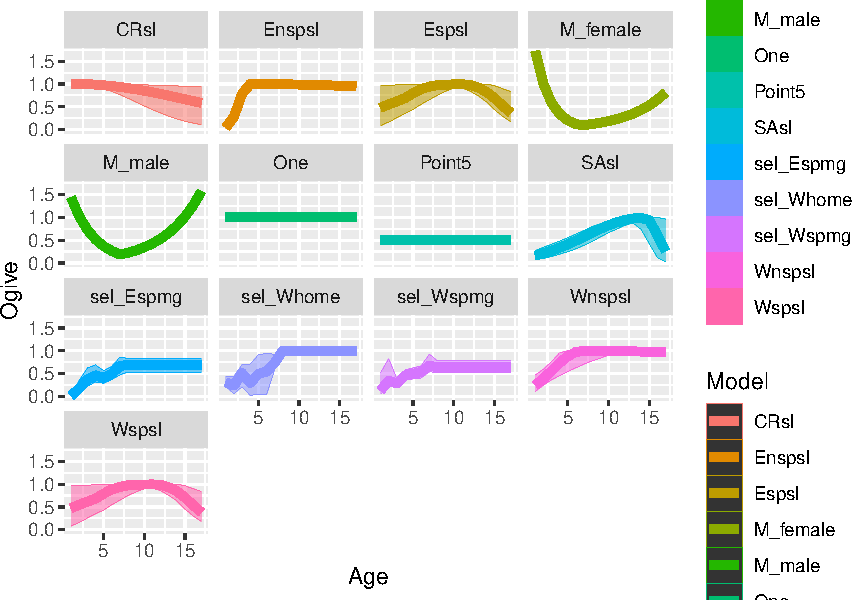
\includegraphics{_main_files/figure-latex/selectivities-1.pdf}

\hypertarget{derived-quantities-1}{%
\subsection{Derived quantities}\label{derived-quantities-1}}

\begin{Shaded}
\begin{Highlighting}[]
\CommentTok{\# plot Ssbs}
\NormalTok{ssbs }\OtherTok{=} \FunctionTok{get\_derived\_quantities}\NormalTok{(}\AttributeTok{model =}\NormalTok{ cas2\_tab)}
\end{Highlighting}
\end{Shaded}

\begin{verbatim}
## getting values for  SSB_E 
## getting values for  SSB_W
\end{verbatim}

\begin{Shaded}
\begin{Highlighting}[]
\CommentTok{\#ssbs\_mpd = get\_derived\_quantities(model = mpd)}
\CommentTok{\#head(ssbs)}
\CommentTok{\#ssbs\_mpd$years = as.numeric(ssbs\_mpd$years)}

\NormalTok{ssbs}\SpecialCharTok{$}\NormalTok{years[ssbs}\SpecialCharTok{$}\NormalTok{years }\SpecialCharTok{==} \StringTok{"initialisation\_phase\_1"}\NormalTok{] }\OtherTok{=} \DecValTok{1971}

\NormalTok{quantile\_ssb\_df }\OtherTok{=}\NormalTok{ ssbs }\SpecialCharTok{\%\textgreater{}\%} 
  \FunctionTok{group\_by}\NormalTok{(years, dq\_label) }\SpecialCharTok{\%\textgreater{}\%} 
  \FunctionTok{summarize\_at}\NormalTok{(}\FunctionTok{vars}\NormalTok{(values), p\_funs)}

\NormalTok{quantile\_ssb\_df}\SpecialCharTok{$}\NormalTok{years }\OtherTok{=} \FunctionTok{as.numeric}\NormalTok{(quantile\_ssb\_df}\SpecialCharTok{$}\NormalTok{years)}
\DocumentationTok{\#\# }
\NormalTok{quant\_ssb\_plot }\OtherTok{=} \FunctionTok{ggplot}\NormalTok{(quantile\_ssb\_df, }\FunctionTok{aes}\NormalTok{(}\AttributeTok{x =}\NormalTok{ years)) }\SpecialCharTok{+} 
  \FunctionTok{geom\_ribbon}\NormalTok{(}\FunctionTok{aes}\NormalTok{(}\AttributeTok{ymax  =}\NormalTok{ low, }\AttributeTok{ymin =}\NormalTok{ upp, }\AttributeTok{alpha =} \FloatTok{0.5}\NormalTok{, }\AttributeTok{col =}\NormalTok{ dq\_label, }\AttributeTok{fill =}\NormalTok{ dq\_label), }\AttributeTok{lwd=}\DecValTok{0}\NormalTok{) }\SpecialCharTok{+}
  \FunctionTok{theme\_bw}\NormalTok{() }\SpecialCharTok{+}
  \FunctionTok{geom\_line}\NormalTok{(}\FunctionTok{aes}\NormalTok{(}\AttributeTok{y =}\NormalTok{ mid, }\AttributeTok{col =}\NormalTok{ dq\_label, }\AttributeTok{group =}\NormalTok{ dq\_label), }\AttributeTok{size =}\DecValTok{2}\NormalTok{, }\AttributeTok{alpha =} \DecValTok{1}\NormalTok{) }\SpecialCharTok{+}
  \FunctionTok{xlab}\NormalTok{(}\StringTok{"Years"}\NormalTok{) }\SpecialCharTok{+}
  \FunctionTok{ylab}\NormalTok{(}\StringTok{"SSB"}\NormalTok{) }\SpecialCharTok{+}
  \FunctionTok{ylim}\NormalTok{(}\DecValTok{0}\NormalTok{, }\DecValTok{2500000}\NormalTok{) }\SpecialCharTok{+}
  \FunctionTok{xlim}\NormalTok{(}\DecValTok{1970}\NormalTok{, }\DecValTok{2020}\NormalTok{) }\SpecialCharTok{+} 
  \FunctionTok{scale\_alpha}\NormalTok{(}\AttributeTok{guide =} \StringTok{\textquotesingle{}none\textquotesingle{}}\NormalTok{) }\SpecialCharTok{+}
  \CommentTok{\#geom\_line(data = ssbs\_mpd, aes(x = years, y = values), inherit.aes = F, col = "black", size = 1.5) +}
  \FunctionTok{facet\_wrap}\NormalTok{(}\SpecialCharTok{\textasciitilde{}}\NormalTok{dq\_label)}
\NormalTok{quant\_ssb\_plot}
\end{Highlighting}
\end{Shaded}

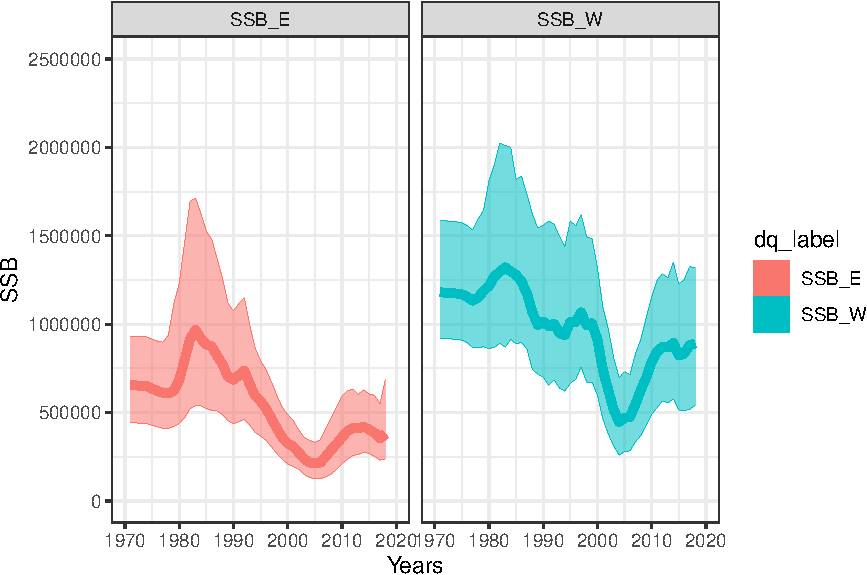
\includegraphics{_main_files/figure-latex/dqs-1.pdf}

\hypertarget{PPC}{%
\chapter{Posterior Predictive Checks}\label{PPC}}

\hypertarget{introduction}{%
\section{Introduction}\label{introduction}}

This vignette demonstrates how to use Casal2s simulation mode with \texttt{r4Casal2} R functions to generate posterior predictive checks for goodness of fit measures. In terms of assessment workflow, this falls in the Diagnostic component.

The following vignette uses the Casal2 model embedded into this R package. If you want to see where this is on you system paste the following line of code into your R console \texttt{system.file("extdata",\ "PosteriorPredictiveChecks",\ package\ =\ "r4Casal2")}

\begin{figure}
\centering
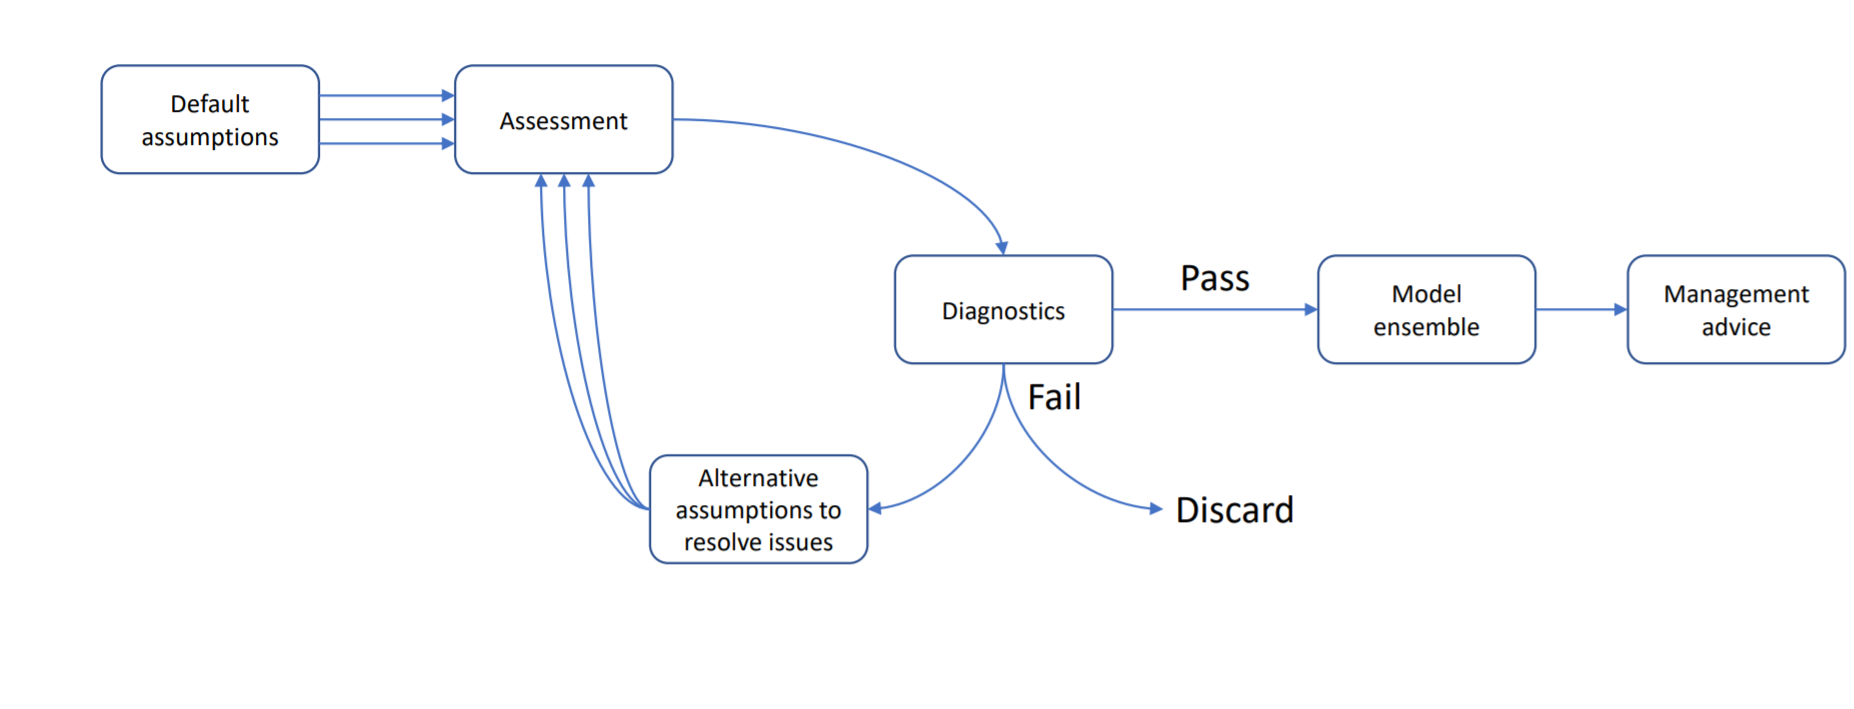
\includegraphics[width=0.5\textwidth,height=\textheight]{Figures/assessment_process.png}
\caption{Assessment Process}
\end{figure}

\hypertarget{estimation}{%
\section{Estimation}\label{estimation}}

Before looking at data goodness of fit you should be checking if the model has converged. We assume that the estimated model has satisfied this criteria i.e.~invertable covariance, acceptable gradient (close to zero) and global minima (as opposed to local - try re-estimating with jittered start values to test for this).

\begin{Shaded}
\begin{Highlighting}[]
\FunctionTok{library}\NormalTok{(DHARMa)}
\FunctionTok{library}\NormalTok{(mvtnorm) }\DocumentationTok{\#\# if simulating obs at MPD}

\NormalTok{mpd\_file\_name }\OtherTok{=} \FunctionTok{system.file}\NormalTok{(}\StringTok{"extdata"}\NormalTok{, }\StringTok{"PosteriorPredictiveChecks"}\NormalTok{,}\StringTok{"estimate.log"}\NormalTok{, }
                            \AttributeTok{package =} \StringTok{"r4Casal2"}\NormalTok{, }\AttributeTok{mustWork =} \ConstantTok{TRUE}\NormalTok{)}
\NormalTok{mpd }\OtherTok{=} \FunctionTok{extract.mpd}\NormalTok{(}\AttributeTok{file =}\NormalTok{ mpd\_file\_name)}
\end{Highlighting}
\end{Shaded}

\begin{verbatim}
## WARNING: The output file was generated with a different version than the R libray being used to read the output.
## This may cause compatibility issues. Please update the R package to be consistent with the version of Casal2 used to generate the output.
## The output was generated with Casal2 v(c) 2
## The Casal2 R package is compatible with Casal2 v23.06
\end{verbatim}

\begin{Shaded}
\begin{Highlighting}[]
\CommentTok{\# Report labels}
\FunctionTok{names}\NormalTok{(mpd)}
\end{Highlighting}
\end{Shaded}

\begin{verbatim}
##  [1] "header"               "obj"                  "estimate_summary"     "covar"               
##  [5] "hess"                 "estimate_value"       "biomass_t1"           "chatOBSest"          
##  [9] "chatOBSwst"           "chatTANage"           "chatTANbiomass"       "Recruitment"         
## [13] "Ageing"               "instant_mort"         "MaturationSel"        "westFSel"            
## [17] "eastFSel"             "chatTANSel"           "One"                  "messages_encountered"
\end{verbatim}

\begin{Shaded}
\begin{Highlighting}[]
\CommentTok{\# is covariance symmetric}
\FunctionTok{isSymmetric}\NormalTok{(mpd}\SpecialCharTok{$}\NormalTok{covar}\SpecialCharTok{$}\NormalTok{covariance\_matrix)}
\end{Highlighting}
\end{Shaded}

\begin{verbatim}
## [1] TRUE
\end{verbatim}

\begin{Shaded}
\begin{Highlighting}[]
\CommentTok{\# is hessian invertable}
\FunctionTok{is\_matrix\_invertable}\NormalTok{(mpd}\SpecialCharTok{$}\NormalTok{hess}\SpecialCharTok{$}\NormalTok{hessian\_matrix)}
\end{Highlighting}
\end{Shaded}

\begin{verbatim}
## [1] TRUE
\end{verbatim}

\hypertarget{simulations}{%
\section{Simulations}\label{simulations}}

The first thing you should do is add reports of type \texttt{simulated\_observation} for each observation in your Casal2 configuration files. The helper function \texttt{?create\_simulation\_reports} will automatically generate a casal2 compatible reports to a file named \texttt{simulated\_reports.csl2} containing all simulated observations in your configuration files. If you use this function you will need to then add an include statement into your Casal2 config files i.e.~\texttt{!include\ simulated\_reports.csl2} before running casal2 in simulation mode \texttt{casal2\ -s\ 1}.

\begin{Shaded}
\begin{Highlighting}[]
\NormalTok{config\_dir }\OtherTok{=} \FunctionTok{system.file}\NormalTok{(}\StringTok{"extdata"}\NormalTok{, }\StringTok{"PosteriorPredictiveChecks"}\NormalTok{, }\AttributeTok{package =} \StringTok{"r4Casal2"}\NormalTok{, }\AttributeTok{mustWork =} \ConstantTok{TRUE}\NormalTok{)}
\NormalTok{config\_files }\OtherTok{=} \StringTok{"Observation.csl2"}
\DocumentationTok{\#\# this will create the file \textquotesingle{}simulated\_reports.csl2\textquotesingle{} in config\_dir}
\DocumentationTok{\#\# in addition to creating the directory labelled output\_folder}
\NormalTok{obs }\OtherTok{=} \FunctionTok{create\_simulation\_reports}\NormalTok{(}\AttributeTok{config\_dir =}\NormalTok{ config\_dir, }\AttributeTok{config\_files =}\NormalTok{ config\_files,}
                                \AttributeTok{output\_folder =} \StringTok{"simulated\_observations"}\NormalTok{)}
\DocumentationTok{\#\# append include statement }
\ControlFlowTok{if}\NormalTok{(}\ConstantTok{FALSE}\NormalTok{)}
  \FunctionTok{cat}\NormalTok{(}\StringTok{"!include simulated\_reports.csl2"}\NormalTok{, }\AttributeTok{file =} 
        \FunctionTok{file.path}\NormalTok{(config\_dir, }\StringTok{"config.csl2"}\NormalTok{), }\AttributeTok{append =}\NormalTok{ T)}
\DocumentationTok{\#\# run Casal2 {-}s}
\CommentTok{\# system(paste0("cd ", config\_dir, "; casal2 {-}s 100 {-}i pars" ))}
\end{Highlighting}
\end{Shaded}

If you don't have these reports in your configuration files, Casal2 will not save simulated observations. Tips when specifying this report class

\begin{enumerate}
\def\labelenumi{\arabic{enumi}.}
\tightlist
\item
  Save each simulated observation into a separate \texttt{file\_name}
\item
  Create a directory to save simulated data sets in.
\item
  Have the report label the same as the \texttt{file\_name} (see example below)
\item
  Avoid the use of periods/dots (``.'') in \texttt{file\_name}
\end{enumerate}

An example report structure would look like

\begin{Shaded}
\begin{Highlighting}[]
\ExtensionTok{@report}\NormalTok{ sim\_chatTANage}
\BuiltInTok{type}\NormalTok{ simulated\_observation}
\ExtensionTok{observation}\NormalTok{ chatTANage}
\ExtensionTok{file\_name}\NormalTok{ simulated\_observations/sim\_chatTANage}
\end{Highlighting}
\end{Shaded}

There are three variants of simulations you can conduct in Casal2, and these depend on if you are in MPD or MCMC estimation phase. If you are evaluating a MPD run, there are two variants and depend if you want to account for parameter uncertainty or not. If you don't want parameter uncertainty, then you need to run the following Casal2 command to produce 100 sets of simulations \texttt{casal2\ -s\ 100\ -i\ mpd\_pars.log\ \textgreater{}\ simulate.log}. If you want to account for parameter uncertainty then you can use a multivariant normal distribution with mean equal to MPD and resulting covariance to produce a set of simulations, example below.

\begin{Shaded}
\begin{Highlighting}[]
\NormalTok{n\_sims }\OtherTok{=} \DecValTok{1000}
\DocumentationTok{\#\# }\AlertTok{NOTE}\DocumentationTok{: might have issue with bounds assuming normal dist}
\NormalTok{sims }\OtherTok{=} \FunctionTok{rmvnorm}\NormalTok{(}\AttributeTok{n =}\NormalTok{ n\_sims, }\AttributeTok{mean =} \FunctionTok{as.numeric}\NormalTok{(mpd}\SpecialCharTok{$}\NormalTok{estimate\_value}\SpecialCharTok{$}\NormalTok{values), }
               \AttributeTok{sigma =}\NormalTok{ mpd}\SpecialCharTok{$}\NormalTok{covar}\SpecialCharTok{$}\NormalTok{covariance\_matrix)}
\FunctionTok{dim}\NormalTok{(sims)}
\end{Highlighting}
\end{Shaded}

\begin{verbatim}
## [1] 1000   46
\end{verbatim}

\begin{Shaded}
\begin{Highlighting}[]
\FunctionTok{colnames}\NormalTok{(sims) }\OtherTok{=} \FunctionTok{names}\NormalTok{(mpd}\SpecialCharTok{$}\NormalTok{estimate\_value}\SpecialCharTok{$}\NormalTok{values)}
\DocumentationTok{\#\# save simulated pars in the same directory as your}
\DocumentationTok{\#\# CSL files}
\ControlFlowTok{if}\NormalTok{(}\ConstantTok{FALSE}\NormalTok{)}
  \FunctionTok{write.table}\NormalTok{(sims, }\AttributeTok{file =} \StringTok{"mpd\_mvnorm\_pars.csl2"}\NormalTok{, }\AttributeTok{quote =}\NormalTok{ F, }\AttributeTok{row.names =}\NormalTok{ F, }\AttributeTok{col.names =}\NormalTok{ T)}
\CommentTok{\# run }
\CommentTok{\# casal2 {-}s 1 {-}i mpd\_mvnorm\_pars.csl2 \textgreater{} simulate.log}
\end{Highlighting}
\end{Shaded}

\hypertarget{summarising-simulated-data-in-r}{%
\section{Summarising simulated data in R}\label{summarising-simulated-data-in-r}}

Assuming you have saved all the simulated observations as separate files in a standalone folder.

\begin{Shaded}
\begin{Highlighting}[]
\NormalTok{sim\_dir }\OtherTok{=} \FunctionTok{system.file}\NormalTok{(}\StringTok{"extdata"}\NormalTok{, }\StringTok{"PosteriorPredictiveChecks"}\NormalTok{,}\StringTok{"simulated\_observations"}\NormalTok{, }
                      \AttributeTok{package =} \StringTok{"r4Casal2"}\NormalTok{, }\AttributeTok{mustWork =} \ConstantTok{TRUE}\NormalTok{)}

\DocumentationTok{\#\# created from running simulations and reading them in with}
\CommentTok{\# sim\_vals = read.simulated.data(dir = sim\_dir, mean\_age = F)}
\CommentTok{\# saveRDS(sim\_vals, file.path("sim\_vals.RDS"))}
\NormalTok{sim\_vals }\OtherTok{=} \FunctionTok{readRDS}\NormalTok{(}\FunctionTok{file.path}\NormalTok{(sim\_dir, }\StringTok{"sim\_vals.RDS"}\NormalTok{))}

\CommentTok{\# check no trouble with files}
\NormalTok{sim\_vals}\SpecialCharTok{$}\NormalTok{failed\_files}
\end{Highlighting}
\end{Shaded}

\begin{verbatim}
## logical(0)
\end{verbatim}

\begin{Shaded}
\begin{Highlighting}[]
\CommentTok{\# }
\FunctionTok{names}\NormalTok{(sim\_vals}\SpecialCharTok{$}\NormalTok{sim\_obs)}
\end{Highlighting}
\end{Shaded}

\begin{verbatim}
## [1] "sim_chatOBSest"     "sim_chatOBSwst"     "sim_chatTANage"     "sim_chatTANbiomass"
\end{verbatim}

\begin{Shaded}
\begin{Highlighting}[]
\NormalTok{sim\_dir\_alt }\OtherTok{=} \FunctionTok{system.file}\NormalTok{(}\StringTok{"extdata"}\NormalTok{, }\StringTok{"PosteriorPredictiveChecks"}\NormalTok{,}\StringTok{"simulated\_observations\_no\_param\_var"}\NormalTok{, }
                          \AttributeTok{package =} \StringTok{"r4Casal2"}\NormalTok{, }\AttributeTok{mustWork =} \ConstantTok{TRUE}\NormalTok{)}

\CommentTok{\#sim\_vals\_alt = read.simulated.data(dir = sim\_dir\_alt, mean\_age = F)}
\CommentTok{\#saveRDS(sim\_vals\_alt, file.path("sim\_vals\_alt.RDS"))}
\NormalTok{sim\_vals\_alt }\OtherTok{=} \FunctionTok{readRDS}\NormalTok{(}\FunctionTok{file.path}\NormalTok{(sim\_dir\_alt, }\StringTok{"sim\_vals\_alt.RDS"}\NormalTok{))}

\CommentTok{\# check no trouble with reading in files}
\NormalTok{sim\_vals\_alt}\SpecialCharTok{$}\NormalTok{failed\_files}
\end{Highlighting}
\end{Shaded}

\begin{verbatim}
## logical(0)
\end{verbatim}

\begin{Shaded}
\begin{Highlighting}[]
\CommentTok{\# }
\FunctionTok{names}\NormalTok{(sim\_vals\_alt}\SpecialCharTok{$}\NormalTok{sim\_obs)}
\end{Highlighting}
\end{Shaded}

\begin{verbatim}
## [1] "sim_chatOBSest"     "sim_chatOBSwst"     "sim_chatTANage"     "sim_chatTANbiomass"
\end{verbatim}

\hypertarget{posterior-predictive-checks}{%
\section{Posterior predictive checks}\label{posterior-predictive-checks}}

Once simulated data has been read into the R environment, we want to compare where the observed values fall relative to the posterior predictive distributions. We recommend using the DHarma r package for this. To interpret P-values or understand the test-statistics that DHARMa does copy this into your R console \texttt{vignette("DHARMa",\ package="DHARMa")} (Assuming you have installed this package).

\begin{Shaded}
\begin{Highlighting}[]
\DocumentationTok{\#\# Create DHARMa objects and P{-}values}
\NormalTok{DHARMaResbio }\OtherTok{=} \FunctionTok{createDHARMa}\NormalTok{(}\AttributeTok{simulatedResponse =}\NormalTok{ sim\_vals}\SpecialCharTok{$}\NormalTok{sim\_obs}\SpecialCharTok{$}\NormalTok{sim\_chatTANbiomass, }
  \AttributeTok{observedResponse =}\NormalTok{ mpd}\SpecialCharTok{$}\NormalTok{chatTANbiomass}\SpecialCharTok{$}\NormalTok{Values}\SpecialCharTok{$}\NormalTok{observed, }
  \AttributeTok{fittedPredictedResponse =}\NormalTok{ mpd}\SpecialCharTok{$}\NormalTok{chatTANbiomass}\SpecialCharTok{$}\NormalTok{Values}\SpecialCharTok{$}\NormalTok{expected, }\AttributeTok{integerResponse =}\NormalTok{ F)}
\DocumentationTok{\#\# Create DHARMa objects and P{-}values}
\DocumentationTok{\#\# for AF }
\NormalTok{mpd}\SpecialCharTok{$}\NormalTok{chatTANage}\SpecialCharTok{$}\NormalTok{Values}\SpecialCharTok{$}\NormalTok{numbers\_at\_age }\OtherTok{=}\NormalTok{ mpd}\SpecialCharTok{$}\NormalTok{chatTANage}\SpecialCharTok{$}\NormalTok{Values}\SpecialCharTok{$}\NormalTok{observed }\SpecialCharTok{*}\NormalTok{ mpd}\SpecialCharTok{$}\NormalTok{chatTANage}\SpecialCharTok{$}\NormalTok{Values}\SpecialCharTok{$}\NormalTok{error\_value}
\NormalTok{year }\OtherTok{=} \DecValTok{1999}
\NormalTok{obs }\OtherTok{=}\NormalTok{ mpd}\SpecialCharTok{$}\NormalTok{chatTANage}\SpecialCharTok{$}\NormalTok{Values}\SpecialCharTok{$}\NormalTok{numbers\_at\_age[mpd}\SpecialCharTok{$}\NormalTok{chatTANage}\SpecialCharTok{$}\NormalTok{Values}\SpecialCharTok{$}\NormalTok{year }\SpecialCharTok{==}\NormalTok{ year]}
\NormalTok{DHARMaResAF }\OtherTok{=} \FunctionTok{createDHARMa}\NormalTok{(}\AttributeTok{simulatedResponse =}\NormalTok{ sim\_vals}\SpecialCharTok{$}\NormalTok{sim\_obs}\SpecialCharTok{$}\NormalTok{sim\_chatTANage[[}\FunctionTok{as.character}\NormalTok{(year)]], }\AttributeTok{observedResponse =}\NormalTok{ obs, }
  \AttributeTok{fittedPredictedResponse =} \ConstantTok{NULL}\NormalTok{, }\AttributeTok{integerResponse =}\NormalTok{ F)}
\end{Highlighting}
\end{Shaded}

\begin{verbatim}
## No fitted predicted response provided, using the mean of the simulations
\end{verbatim}

\begin{Shaded}
\begin{Highlighting}[]
\DocumentationTok{\#\# use DHARMa functions}
\FunctionTok{plot}\NormalTok{(DHARMaResbio, }\AttributeTok{quantreg =}\NormalTok{ F)}
\end{Highlighting}
\end{Shaded}

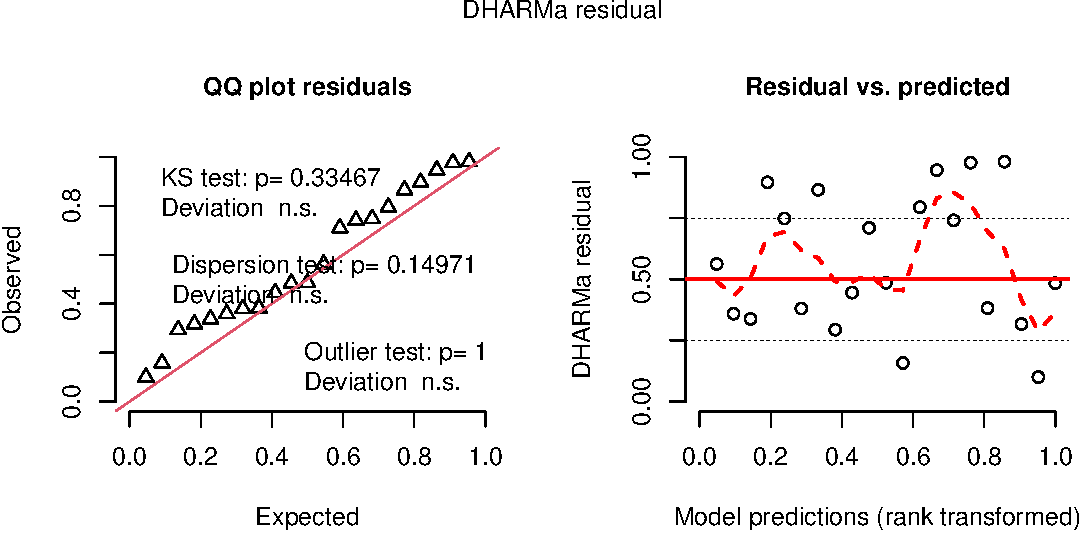
\includegraphics{_main_files/figure-latex/ppp-1.pdf}

\begin{Shaded}
\begin{Highlighting}[]
\FunctionTok{plot}\NormalTok{(DHARMaResAF, }\AttributeTok{quantreg =}\NormalTok{ F)}
\end{Highlighting}
\end{Shaded}

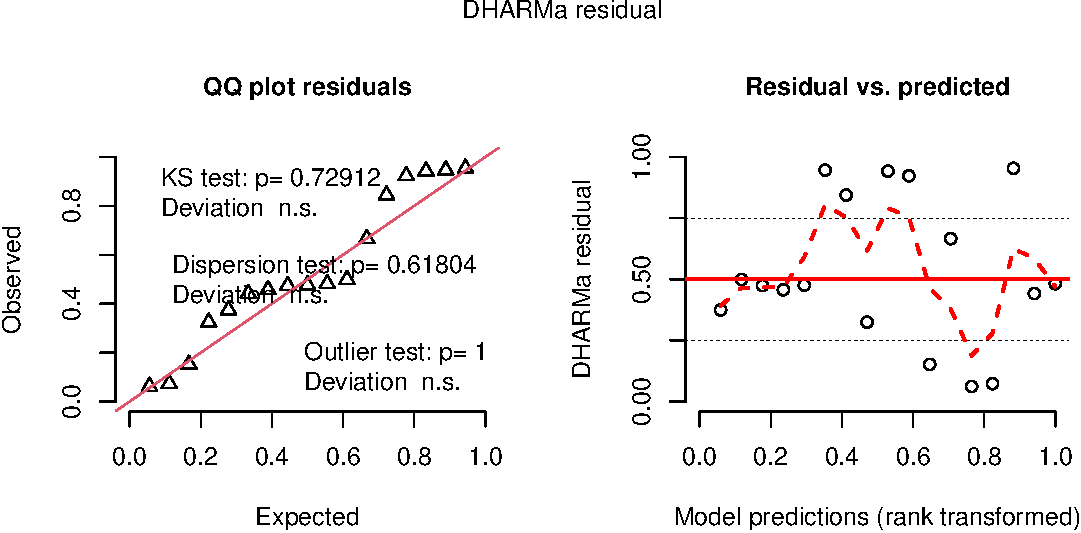
\includegraphics{_main_files/figure-latex/ppp-2.pdf}

Examples of custom plots

\begin{Shaded}
\begin{Highlighting}[]
\NormalTok{sim\_chatTANbiomass }\OtherTok{=}\NormalTok{ sim\_vals}\SpecialCharTok{$}\NormalTok{sim\_obs}\SpecialCharTok{$}\NormalTok{sim\_chatTANbiomass}
\FunctionTok{rownames}\NormalTok{(sim\_chatTANbiomass) }\OtherTok{=}\NormalTok{ mpd}\SpecialCharTok{$}\NormalTok{chatTANbiomass}\SpecialCharTok{$}\NormalTok{Values}\SpecialCharTok{$}\NormalTok{year}
\NormalTok{DHARMaResbio\_quant\_resids }\OtherTok{=} \FunctionTok{createDHARMa}\NormalTok{(}\AttributeTok{simulatedResponse =}\NormalTok{ sim\_chatTANbiomass, }
                            \AttributeTok{observedResponse =}\NormalTok{ mpd}\SpecialCharTok{$}\NormalTok{chatTANbiomass}\SpecialCharTok{$}\NormalTok{Values}\SpecialCharTok{$}\NormalTok{observed, }
                            \AttributeTok{fittedPredictedResponse =}\NormalTok{ mpd}\SpecialCharTok{$}\NormalTok{chatTANbiomass}\SpecialCharTok{$}\NormalTok{Values}\SpecialCharTok{$}\NormalTok{expected, }\AttributeTok{integerResponse =}\NormalTok{ F)}
\DocumentationTok{\#\# convert from uniform variable {-}\textgreater{} standard normal}
\NormalTok{norm\_quant\_resids }\OtherTok{=} \FunctionTok{qnorm}\NormalTok{(DHARMaResbio\_quant\_resids}\SpecialCharTok{$}\NormalTok{scaledResiduals)}
\CommentTok{\# formal tests}
\CommentTok{\#dispersion\_test = testDispersion(DHARMaResbio\_quant\_resids)}
\CommentTok{\#zero\_inflat\_test = testZeroInflation(DHARMaResbio\_quant\_resids)}
\NormalTok{temporal\_correlation }\OtherTok{=} \FunctionTok{testTemporalAutocorrelation}\NormalTok{(}\AttributeTok{simulationOutput =}\NormalTok{ DHARMaResbio\_quant\_resids, }\AttributeTok{time =}\NormalTok{ mpd}\SpecialCharTok{$}\NormalTok{chatTANbiomass}\SpecialCharTok{$}\NormalTok{Values}\SpecialCharTok{$}\NormalTok{year, }\AttributeTok{plot =}\NormalTok{ F) }\DocumentationTok{\#\# HO: rho = 0, HA: rho != 0}
\NormalTok{temporal\_correlation}
\end{Highlighting}
\end{Shaded}

\begin{verbatim}
## 
##  Durbin-Watson test
## 
## data:  simulationOutput$scaledResiduals ~ 1
## DW = 1.9861, p-value = 0.9743
## alternative hypothesis: true autocorrelation is not 0
\end{verbatim}

\begin{Shaded}
\begin{Highlighting}[]
\DocumentationTok{\#\# plot posterior predictive checks}
\NormalTok{bioplt }\OtherTok{=} \FunctionTok{plot\_abundance\_predictive\_dist}\NormalTok{(}\AttributeTok{sim\_data =}\NormalTok{ sim\_chatTANbiomass, }
                              \AttributeTok{obs =} \FunctionTok{data.frame}\NormalTok{(}\AttributeTok{obs =}\NormalTok{ mpd}\SpecialCharTok{$}\NormalTok{chatTANbiomass}\SpecialCharTok{$}\NormalTok{Values}\SpecialCharTok{$}\NormalTok{observed, }
                                               \AttributeTok{year =}\NormalTok{ mpd}\SpecialCharTok{$}\NormalTok{chatTANbiomass}\SpecialCharTok{$}\NormalTok{Values}\SpecialCharTok{$}\NormalTok{year,}
                                               \AttributeTok{mpd\_fit =}\NormalTok{ mpd}\SpecialCharTok{$}\NormalTok{chatTANbiomass}\SpecialCharTok{$}\NormalTok{Values}\SpecialCharTok{$}\NormalTok{expected),}
                              \AttributeTok{lab =} \StringTok{""}\NormalTok{, }\AttributeTok{plot\_type =} \StringTok{"violin"}\NormalTok{)}
\end{Highlighting}
\end{Shaded}

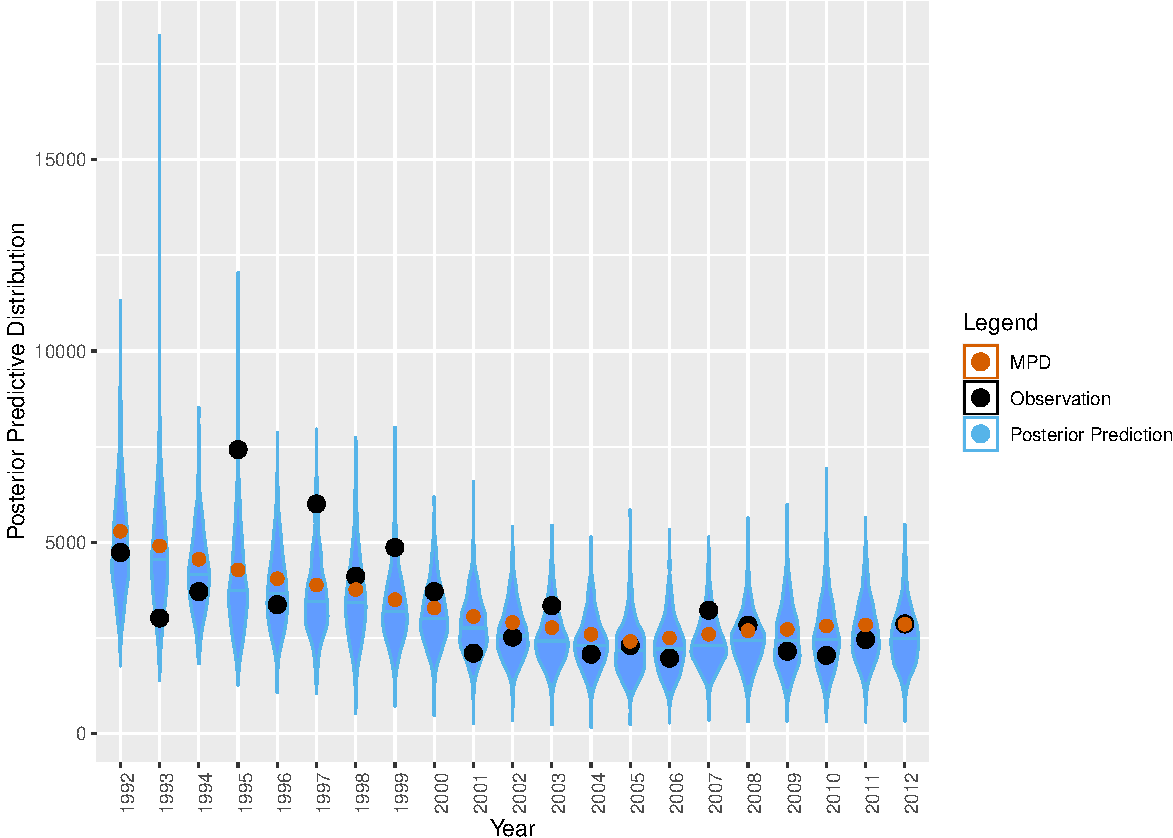
\includegraphics{_main_files/figure-latex/custom_figures-1.pdf}

\begin{Shaded}
\begin{Highlighting}[]
\NormalTok{bioplt}\OtherTok{=}\NormalTok{ bioplt }\SpecialCharTok{+} \FunctionTok{theme}\NormalTok{(}\AttributeTok{axis.text.x =} \FunctionTok{element\_text}\NormalTok{(}\AttributeTok{angle =} \DecValTok{90}\NormalTok{)) }\SpecialCharTok{+}
  \FunctionTok{ggtitle}\NormalTok{(}\StringTok{"MPD Predictive distributions"}\NormalTok{)}
\DocumentationTok{\#\# qq plot for simulated quantile residuals.}
\NormalTok{norm\_resid }\OtherTok{=} \FunctionTok{ggplot}\NormalTok{(}\FunctionTok{data.frame}\NormalTok{(}\AttributeTok{resids =}\NormalTok{ norm\_quant\_resids), }\FunctionTok{aes}\NormalTok{(}\AttributeTok{sample =}\NormalTok{ resids)) }\SpecialCharTok{+}
  \FunctionTok{stat\_qq}\NormalTok{(}\AttributeTok{size =} \DecValTok{3}\NormalTok{) }\SpecialCharTok{+}
  \FunctionTok{stat\_qq\_line}\NormalTok{(}\AttributeTok{col =} \StringTok{"steelblue"}\NormalTok{, }\AttributeTok{size =} \FloatTok{1.5}\NormalTok{, }\AttributeTok{linetype =} \StringTok{"dashed"}\NormalTok{) }\SpecialCharTok{+}
  \FunctionTok{labs}\NormalTok{(}\AttributeTok{x =} \StringTok{"Theoretical"}\NormalTok{, }\AttributeTok{y =} \StringTok{"Sample"}\NormalTok{)}
\DocumentationTok{\#\# Plot normalised residuals generated from Casal2}
\NormalTok{normalised\_resids }\OtherTok{=} \FunctionTok{ggplot}\NormalTok{(mpd}\SpecialCharTok{$}\NormalTok{chatTANbiomass}\SpecialCharTok{$}\NormalTok{Values, }\FunctionTok{aes}\NormalTok{(}\AttributeTok{sample =}\NormalTok{ normalised\_residuals)) }\SpecialCharTok{+}
  \FunctionTok{stat\_qq}\NormalTok{(}\AttributeTok{size =} \DecValTok{3}\NormalTok{) }\SpecialCharTok{+}
  \FunctionTok{stat\_qq\_line}\NormalTok{(}\AttributeTok{col =} \StringTok{"steelblue"}\NormalTok{, }\AttributeTok{size =} \FloatTok{1.5}\NormalTok{, }\AttributeTok{linetype =} \StringTok{"dashed"}\NormalTok{) }\SpecialCharTok{+}
  \FunctionTok{labs}\NormalTok{(}\AttributeTok{x =} \StringTok{"Theoretical"}\NormalTok{, }\AttributeTok{y =} \StringTok{"Sample"}\NormalTok{)}
\DocumentationTok{\#\# Plot fits obs}
\NormalTok{fits }\OtherTok{=} \FunctionTok{plot\_relative\_index}\NormalTok{(}\AttributeTok{model =}\NormalTok{ mpd, }\AttributeTok{report\_label =} \StringTok{"chatTANbiomass"}\NormalTok{) }\SpecialCharTok{+} \FunctionTok{ggtitle}\NormalTok{(}\StringTok{""}\NormalTok{)}
\DocumentationTok{\#\#}
\NormalTok{fits}
\end{Highlighting}
\end{Shaded}

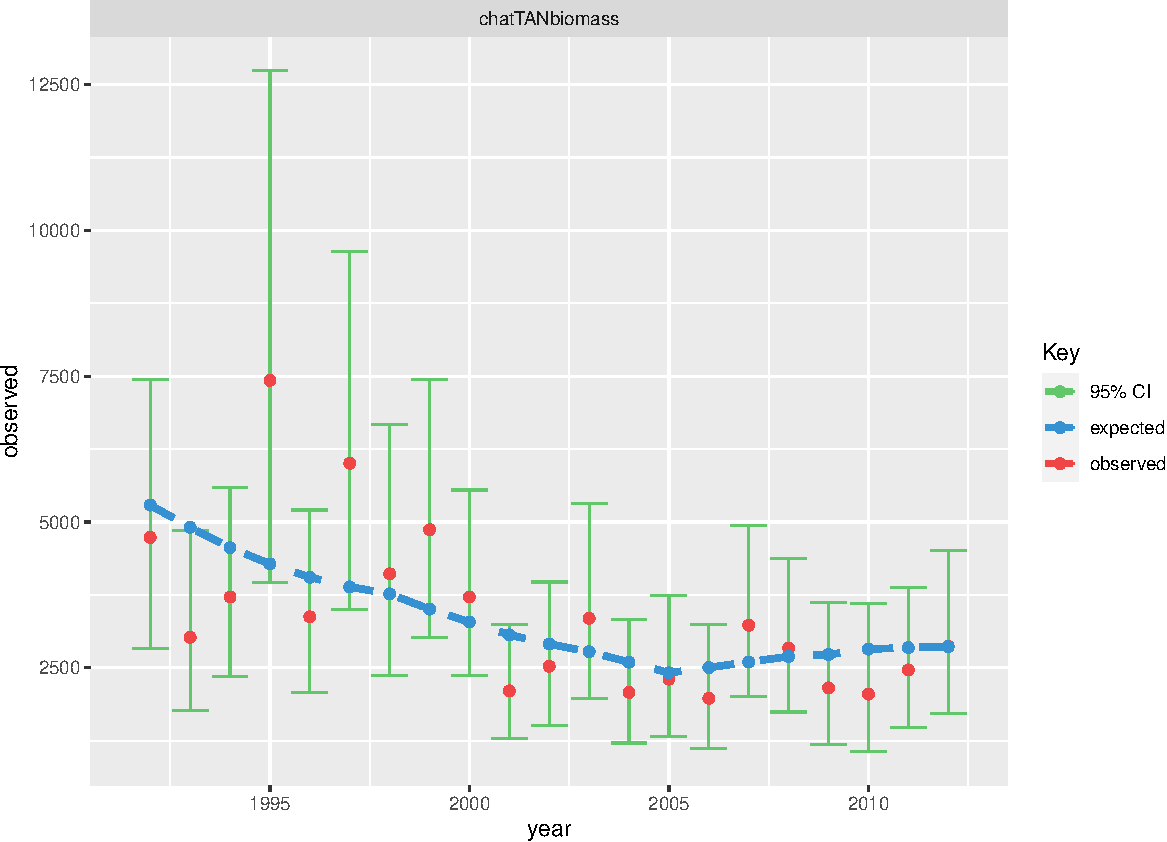
\includegraphics{_main_files/figure-latex/custom_figures-2.pdf}

Look at Predictive checks when generated with variability in parameter estimates as well.

\begin{Shaded}
\begin{Highlighting}[]
\DocumentationTok{\#\# Create DHARMa objects and P{-}values}
\NormalTok{DHARMaResbio }\OtherTok{=} \FunctionTok{createDHARMa}\NormalTok{(}\AttributeTok{simulatedResponse =}\NormalTok{ sim\_vals\_alt}\SpecialCharTok{$}\NormalTok{sim\_obs}\SpecialCharTok{$}\NormalTok{sim\_chatTANbiomass, }
  \AttributeTok{observedResponse =}\NormalTok{ mpd}\SpecialCharTok{$}\NormalTok{chatTANbiomass}\SpecialCharTok{$}\NormalTok{Values}\SpecialCharTok{$}\NormalTok{observed, }
  \AttributeTok{fittedPredictedResponse =}\NormalTok{ mpd}\SpecialCharTok{$}\NormalTok{chatTANbiomass}\SpecialCharTok{$}\NormalTok{Values}\SpecialCharTok{$}\NormalTok{expected, }\AttributeTok{integerResponse =}\NormalTok{ F)}
\DocumentationTok{\#\# Create DHARMa objects and P{-}values}
\DocumentationTok{\#\# for AF }
\NormalTok{year }\OtherTok{=} \DecValTok{2000}
\NormalTok{obs }\OtherTok{=}\NormalTok{ mpd}\SpecialCharTok{$}\NormalTok{chatTANage}\SpecialCharTok{$}\NormalTok{Values}\SpecialCharTok{$}\NormalTok{numbers\_at\_age[mpd}\SpecialCharTok{$}\NormalTok{chatTANage}\SpecialCharTok{$}\NormalTok{Values}\SpecialCharTok{$}\NormalTok{year }\SpecialCharTok{==}\NormalTok{ year]}

\NormalTok{DHARMaResAF }\OtherTok{=} \FunctionTok{createDHARMa}\NormalTok{(}\AttributeTok{simulatedResponse =}\NormalTok{ sim\_vals\_alt}\SpecialCharTok{$}\NormalTok{sim\_obs}\SpecialCharTok{$}\NormalTok{sim\_chatTANage[[}\FunctionTok{as.character}\NormalTok{(year)]], }\AttributeTok{observedResponse =}\NormalTok{ obs, }
  \AttributeTok{fittedPredictedResponse =} \ConstantTok{NULL}\NormalTok{, }\AttributeTok{integerResponse =}\NormalTok{ T)}
\end{Highlighting}
\end{Shaded}

\begin{verbatim}
## No fitted predicted response provided, using the mean of the simulations
\end{verbatim}

\begin{Shaded}
\begin{Highlighting}[]
\FunctionTok{plot}\NormalTok{(DHARMaResbio, }\AttributeTok{quantreg =}\NormalTok{ F)}
\end{Highlighting}
\end{Shaded}

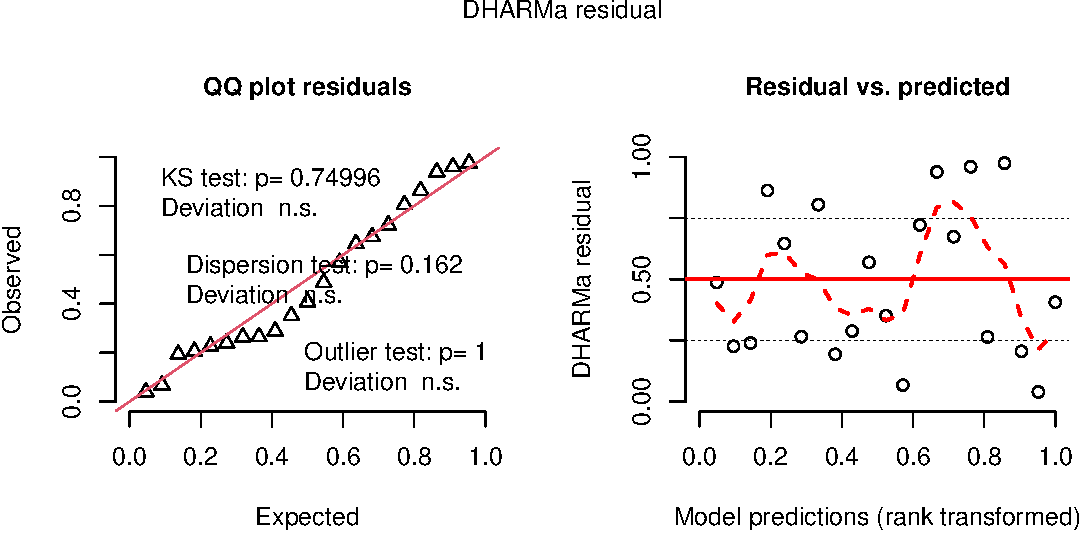
\includegraphics{_main_files/figure-latex/ppp_no_param_var-1.pdf}

\begin{Shaded}
\begin{Highlighting}[]
\FunctionTok{plot}\NormalTok{(DHARMaResAF, }\AttributeTok{quantreg =}\NormalTok{ F)}
\end{Highlighting}
\end{Shaded}

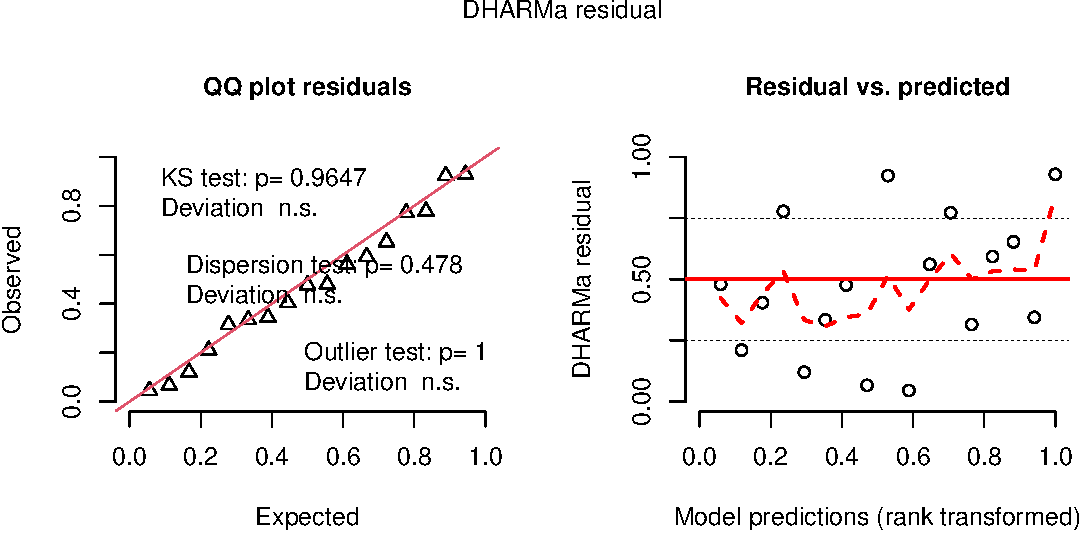
\includegraphics{_main_files/figure-latex/ppp_no_param_var-2.pdf}

Some other visualizations plots

\begin{Shaded}
\begin{Highlighting}[]
\DocumentationTok{\#\#\#\#\#\#\#\#\#\#\#\#\#\#\#\#\#\#\#\#\#\#\#\#}
\DocumentationTok{\#\# boxplot predictive distribution vs observation}
\NormalTok{legend }\OtherTok{=} \FunctionTok{c}\NormalTok{(}\StringTok{"Posterior Prediction"} \OtherTok{=} \StringTok{"\#56B4E9"}\NormalTok{, }\StringTok{"Observation"} \OtherTok{=} \StringTok{"black"}\NormalTok{ , }\StringTok{"MPD"} \OtherTok{=} \StringTok{"\#D55E00"}\NormalTok{)}

\NormalTok{sim\_data }\OtherTok{=}\NormalTok{ sim\_vals}\SpecialCharTok{$}\NormalTok{sim\_obs}\SpecialCharTok{$}\NormalTok{sim\_chatTANbiomass}
\FunctionTok{rownames}\NormalTok{(sim\_data) }\OtherTok{=}\NormalTok{ mpd}\SpecialCharTok{$}\NormalTok{chatTANbiomass}\SpecialCharTok{$}\NormalTok{Values}\SpecialCharTok{$}\NormalTok{year}

\NormalTok{bioplt }\OtherTok{=} \FunctionTok{plot\_abundance\_predictive\_dist}\NormalTok{(}\AttributeTok{sim\_data =}\NormalTok{ sim\_data, }
    \AttributeTok{obs =} \FunctionTok{data.frame}\NormalTok{(}\AttributeTok{obs =}\NormalTok{ mpd}\SpecialCharTok{$}\NormalTok{chatTANbiomass}\SpecialCharTok{$}\NormalTok{Values}\SpecialCharTok{$}\NormalTok{observed, }
    \AttributeTok{year =}\NormalTok{ mpd}\SpecialCharTok{$}\NormalTok{chatTANbiomass}\SpecialCharTok{$}\NormalTok{Values}\SpecialCharTok{$}\NormalTok{year,}
    \AttributeTok{mpd\_fit =}\NormalTok{ mpd}\SpecialCharTok{$}\NormalTok{chatTANbiomass}\SpecialCharTok{$}\NormalTok{Values}\SpecialCharTok{$}\NormalTok{expected), }
    \AttributeTok{lab =} \StringTok{"chatTANbiomass"}\NormalTok{, }\AttributeTok{plot\_type =} \StringTok{"violin"}\NormalTok{)}
\end{Highlighting}
\end{Shaded}

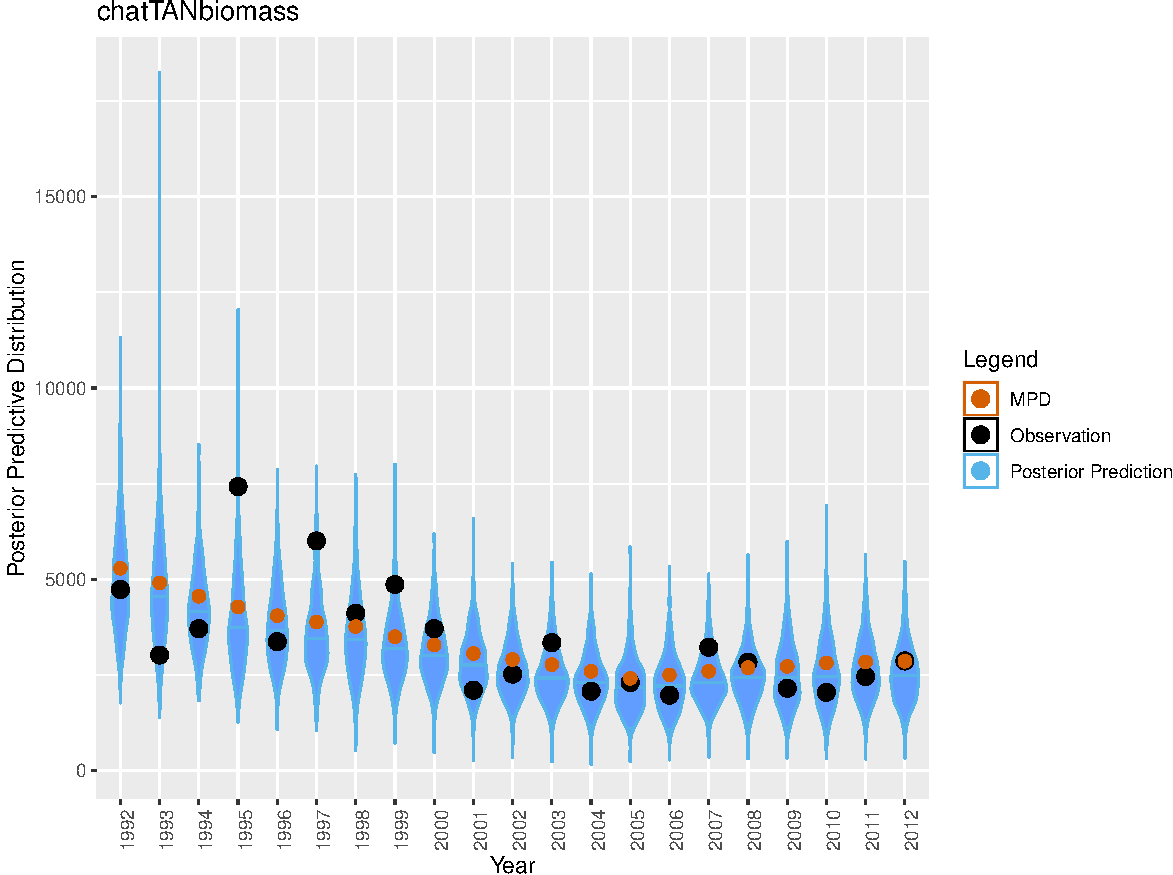
\includegraphics{_main_files/figure-latex/ggplots_ppp-1.pdf}

\begin{Shaded}
\begin{Highlighting}[]
\NormalTok{chat\_sim\_vals }\OtherTok{=} \FunctionTok{get\_simulated\_age\_resids}\NormalTok{(sim\_vals}\SpecialCharTok{$}\NormalTok{sim\_obs}\SpecialCharTok{$}\NormalTok{sim\_chatTANage, mpd}\SpecialCharTok{$}\NormalTok{chatTANage)}
\NormalTok{obs\_years }\OtherTok{=} \FunctionTok{unique}\NormalTok{(chat\_sim\_vals}\SpecialCharTok{$}\NormalTok{mpd\_df}\SpecialCharTok{$}\NormalTok{year)}
\NormalTok{years\_to\_plot }\OtherTok{=}\NormalTok{ obs\_years[}\DecValTok{1}\SpecialCharTok{:}\DecValTok{12}\NormalTok{]}
\NormalTok{pppAFplt\_1 }\OtherTok{=}  \FunctionTok{ggplot}\NormalTok{(chat\_sim\_vals}\SpecialCharTok{$}\NormalTok{full\_simulated\_values }\SpecialCharTok{\%\textgreater{}\%} 
    \FunctionTok{filter}\NormalTok{(year }\SpecialCharTok{\%in\%}\NormalTok{ years\_to\_plot), }\FunctionTok{aes}\NormalTok{(}\AttributeTok{x =} \FunctionTok{factor}\NormalTok{(age, }\AttributeTok{ordered =}\NormalTok{ T), }\AttributeTok{y =}\NormalTok{ simulated\_value)) }\SpecialCharTok{+}
  \FunctionTok{geom\_violin}\NormalTok{(}\FunctionTok{aes}\NormalTok{(}\AttributeTok{color =} \StringTok{"Posterior Prediction"}\NormalTok{, }\AttributeTok{fill =} \StringTok{"Posterior Prediction"}\NormalTok{),}\AttributeTok{adjust=}\DecValTok{2}\NormalTok{) }\SpecialCharTok{+}
  \FunctionTok{scale\_color\_manual}\NormalTok{(}\AttributeTok{values =}\NormalTok{ legend) }\SpecialCharTok{+}
  \FunctionTok{guides}\NormalTok{(}\AttributeTok{fill =} \StringTok{"none"}\NormalTok{) }\SpecialCharTok{+}
  \FunctionTok{theme}\NormalTok{(}\AttributeTok{axis.text.x =} \FunctionTok{element\_text}\NormalTok{(}\AttributeTok{angle =} \DecValTok{45}\NormalTok{)) }\SpecialCharTok{+}
  \FunctionTok{labs}\NormalTok{(}\AttributeTok{colour =} \StringTok{"Legend"}\NormalTok{, }\AttributeTok{x =} \StringTok{"Age"}\NormalTok{, }\AttributeTok{y =} \StringTok{"Posterior Predictive Distribution"}\NormalTok{) }\SpecialCharTok{+}
  \FunctionTok{geom\_point}\NormalTok{(}\AttributeTok{data =}\NormalTok{ chat\_sim\_vals}\SpecialCharTok{$}\NormalTok{mpd\_df }\SpecialCharTok{\%\textgreater{}\%} \FunctionTok{filter}\NormalTok{(year }\SpecialCharTok{\%in\%}\NormalTok{ years\_to\_plot), }\FunctionTok{aes}\NormalTok{(}\AttributeTok{x =} \FunctionTok{factor}\NormalTok{(age, }\AttributeTok{ordered =}\NormalTok{ T), }\AttributeTok{y =}\NormalTok{ observed }\SpecialCharTok{*}\NormalTok{ error\_value, }\AttributeTok{color =} \StringTok{"Observation"}\NormalTok{, }\AttributeTok{fill =} \StringTok{"Observation"}\NormalTok{), }\AttributeTok{size =} \FloatTok{2.4}\NormalTok{, }\AttributeTok{inherit.aes =}\NormalTok{ F ) }\SpecialCharTok{+}
  \FunctionTok{facet\_wrap}\NormalTok{(}\SpecialCharTok{\textasciitilde{}}\NormalTok{year, }\AttributeTok{scales =} \StringTok{"free\_y"}\NormalTok{, }\AttributeTok{ncol =} \DecValTok{3}\NormalTok{)    }\SpecialCharTok{+}
  \FunctionTok{ggtitle}\NormalTok{(}\StringTok{"chatTANage"}\NormalTok{)}
\NormalTok{pppAFplt\_1}
\end{Highlighting}
\end{Shaded}

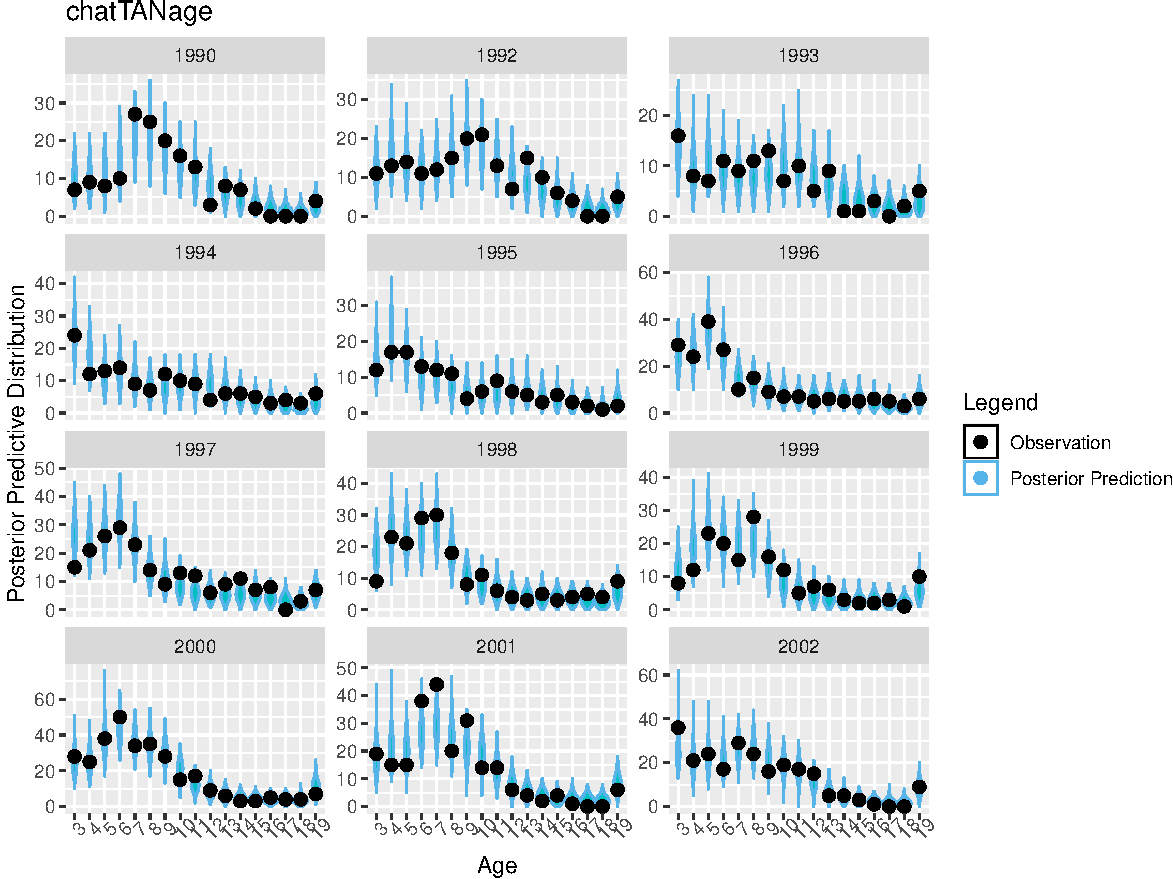
\includegraphics{_main_files/figure-latex/ggplots_ppp-2.pdf}

\begin{Shaded}
\begin{Highlighting}[]
\NormalTok{OM\_file }\OtherTok{=} \FunctionTok{system.file}\NormalTok{(}\StringTok{"extdata"}\NormalTok{, }\StringTok{"PosteriorPredictiveChecks"}\NormalTok{,}\StringTok{"OM"}\NormalTok{,}\StringTok{"OM\_vary.log"}\NormalTok{, }\AttributeTok{package =} \StringTok{"r4Casal2"}\NormalTok{, }\AttributeTok{mustWork =} \ConstantTok{TRUE}\NormalTok{)}
\NormalTok{OM\_run }\OtherTok{=} \FunctionTok{extract.mpd}\NormalTok{(}\AttributeTok{file =}\NormalTok{ OM\_file)}
\end{Highlighting}
\end{Shaded}

\begin{verbatim}
## WARNING: The output file was generated with a different version than the R libray being used to read the output.
## This may cause compatibility issues. Please update the R package to be consistent with the version of Casal2 used to generate the output.
## The output was generated with Casal2 v(c) 2
## The Casal2 R package is compatible with Casal2 v23.06
## 
## loading a Casal2 output from a multi parameter input format
## loading a Casal2 output from a multi parameter input format
\end{verbatim}

\begin{Shaded}
\begin{Highlighting}[]
\DocumentationTok{\#\# plot SSBs}
\NormalTok{my\_plot }\OtherTok{=}\NormalTok{ r4Casal2}\SpecialCharTok{::}\FunctionTok{plot\_derived\_quantities}\NormalTok{(}\AttributeTok{model =} \FunctionTok{list}\NormalTok{(}\AttributeTok{OM =}\NormalTok{ OM\_run, }\AttributeTok{EM =}\NormalTok{ mpd))}
\NormalTok{my\_plot }\OtherTok{=}\NormalTok{ my\_plot }\SpecialCharTok{+} \FunctionTok{xlab}\NormalTok{(}\StringTok{"SSB"}\NormalTok{) }\SpecialCharTok{+} \FunctionTok{ylim}\NormalTok{(}\DecValTok{0}\NormalTok{, }\DecValTok{120000}\NormalTok{)}
\end{Highlighting}
\end{Shaded}

\begin{verbatim}
## Scale for y is already present.
## Adding another scale for y, which will replace the existing scale.
\end{verbatim}

\hypertarget{pit-residuals}{%
\section{PIT residuals}\label{pit-residuals}}

Pearson residuals for multinomial distributed random variables can be difficult to interpret for a lot of reasons, data-weighting for mean age to standardised residuals = 1 \citep{francis2011data}, sparsity can create funny patterns etc. An alternative is to use randomised quantile PIT residuals \citep{warton2017pit, dunn1996randomized}

Assuming we have data denoted by \(y\) which has cumulative distribution function \(F(y; \theta), u = F(y; \theta) \sim Uniform(0,1)\). For discrete variables the following adjustment can be made
\begin{align}
u_i = q_i F(y; \theta) + (1 - q_i) F(y^{-}; \theta) 
\end{align}
where, \(q_i\) is a standard uniform random variable and \(y^{-}\) is the previous allowable value for \(y\).
they do not behave like residuals in the usual sense they are centred around a value of 0.5 rather than a value of 0, and are bounded between 0 and 1.

\begin{Shaded}
\begin{Highlighting}[]
\CommentTok{\# hello}
\FunctionTok{set.seed}\NormalTok{(}\DecValTok{123}\NormalTok{)}
\NormalTok{n }\OtherTok{=} \DecValTok{50}
\NormalTok{nsims }\OtherTok{=} \DecValTok{1000}
\NormalTok{x }\OtherTok{=} \FunctionTok{rnorm}\NormalTok{(n, }\DecValTok{5}\NormalTok{, }\DecValTok{3}\NormalTok{)}
\NormalTok{beta0 }\OtherTok{=} \DecValTok{3}
\NormalTok{beta1 }\OtherTok{=} \FloatTok{1.2}
\NormalTok{true\_beta1 }\OtherTok{=} \DecValTok{1}
\NormalTok{y }\OtherTok{=} \FunctionTok{rpois}\NormalTok{(n, beta0 }\SpecialCharTok{+}\NormalTok{ true\_beta1 }\SpecialCharTok{*}\NormalTok{ x)}
\NormalTok{y\_sim }\OtherTok{=} \FunctionTok{matrix}\NormalTok{(}\AttributeTok{nrow =}\NormalTok{ n, }\AttributeTok{ncol =}\NormalTok{ nsims) }
\ControlFlowTok{for}\NormalTok{(i }\ControlFlowTok{in} \DecValTok{1}\SpecialCharTok{:}\NormalTok{nsims)}
\NormalTok{  y\_sim[,i] }\OtherTok{=} \FunctionTok{rpois}\NormalTok{(n, beta0 }\SpecialCharTok{+}\NormalTok{ beta1 }\SpecialCharTok{*}\NormalTok{ x)}
\DocumentationTok{\#\# calculate PIT}
\NormalTok{PITResiduals }\OtherTok{=} \FunctionTok{rep}\NormalTok{(}\ConstantTok{NA}\NormalTok{, n)}
\NormalTok{altPITResiduals }\OtherTok{=} \FunctionTok{rep}\NormalTok{(}\ConstantTok{NA}\NormalTok{, n)}
\ControlFlowTok{for}\NormalTok{ (i }\ControlFlowTok{in} \DecValTok{1}\SpecialCharTok{:}\NormalTok{n)\{}
\NormalTok{  minSim }\OtherTok{\textless{}{-}} \FunctionTok{mean}\NormalTok{(y\_sim[i,] }\SpecialCharTok{\textless{}}\NormalTok{ y[i]) }
\NormalTok{  maxSim }\OtherTok{\textless{}{-}} \FunctionTok{mean}\NormalTok{(y\_sim[i,] }\SpecialCharTok{\textless{}=}\NormalTok{ y[i]) }
  \ControlFlowTok{if}\NormalTok{ (minSim }\SpecialCharTok{==}\NormalTok{ maxSim) \{}
\NormalTok{    PITResiduals[i] }\OtherTok{=}\NormalTok{ minSim}
\NormalTok{  \} }\ControlFlowTok{else}\NormalTok{ \{}
\NormalTok{    PITResiduals[i] }\OtherTok{=} \FunctionTok{runif}\NormalTok{(}\DecValTok{1}\NormalTok{, minSim, maxSim)}
\NormalTok{  \}}
\NormalTok{  qi }\OtherTok{=} \FunctionTok{runif}\NormalTok{(}\DecValTok{1}\NormalTok{)}
\NormalTok{  lower\_limit }\OtherTok{=} \FunctionTok{mean}\NormalTok{(y\_sim[i,] }\SpecialCharTok{\textless{}}\NormalTok{ y[i])}
\NormalTok{  cum\_ecdf }\OtherTok{=} \FunctionTok{mean}\NormalTok{(y\_sim[i,] }\SpecialCharTok{\textless{}=}\NormalTok{ y[i])}
\NormalTok{  altPITResiduals[i] }\OtherTok{=}\NormalTok{ qi }\SpecialCharTok{*}\NormalTok{ cum\_ecdf }\SpecialCharTok{+}\NormalTok{ (}\DecValTok{1} \SpecialCharTok{{-}}\NormalTok{ qi) }\SpecialCharTok{*}\NormalTok{ lower\_limit}
\NormalTok{\}}
\FunctionTok{plot}\NormalTok{(PITResiduals, altPITResiduals)}
\end{Highlighting}
\end{Shaded}

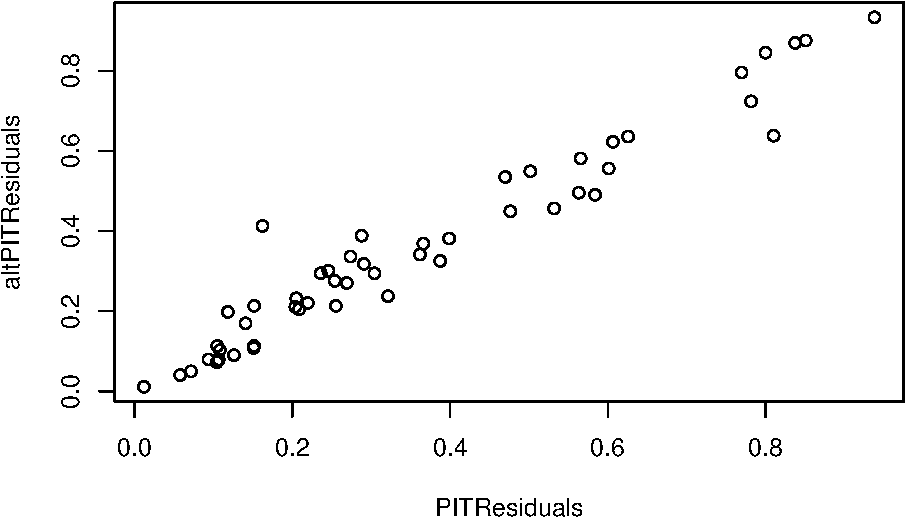
\includegraphics{_main_files/figure-latex/illustrate_PIT-1.pdf}

\begin{Shaded}
\begin{Highlighting}[]
\CommentTok{\# It is assumed that PIT residuals are from uniform(0,1)}
\CommentTok{\# most people transform them to normal distribution for testing}
\CommentTok{\# for familiarity more than anything.}
\NormalTok{normal\_transformed }\OtherTok{=} \FunctionTok{qnorm}\NormalTok{(PITResiduals)}
\FunctionTok{qqnorm}\NormalTok{(normal\_transformed)}
\FunctionTok{qqline}\NormalTok{(normal\_transformed, }\AttributeTok{col =} \StringTok{"steelblue"}\NormalTok{, }\AttributeTok{lwd =} \DecValTok{3}\NormalTok{, }\AttributeTok{lty =} \DecValTok{2}\NormalTok{)}
\end{Highlighting}
\end{Shaded}

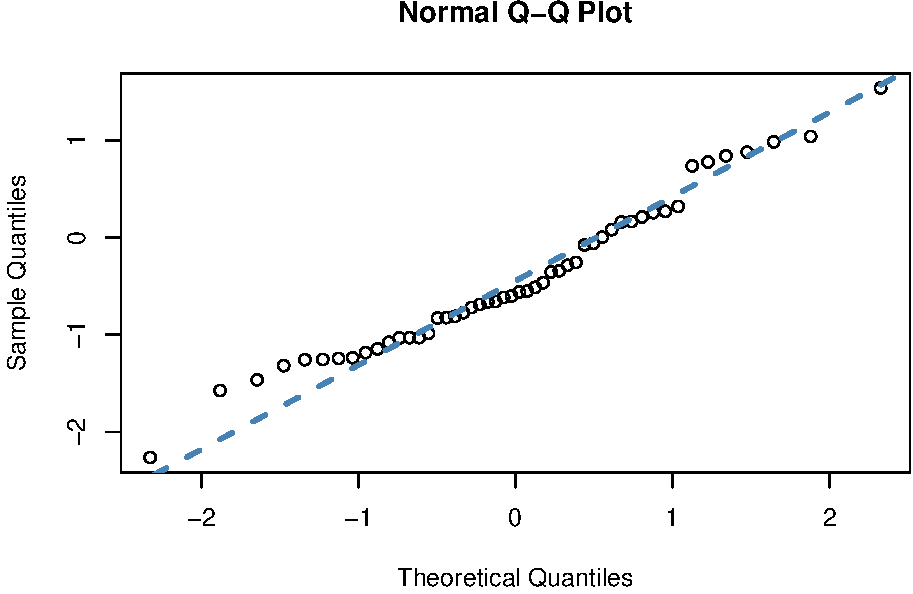
\includegraphics{_main_files/figure-latex/illustrate_PIT-2.pdf}

\begin{Shaded}
\begin{Highlighting}[]
\FunctionTok{shapiro.test}\NormalTok{(normal\_transformed)}
\end{Highlighting}
\end{Shaded}

\begin{verbatim}
## 
##  Shapiro-Wilk normality test
## 
## data:  normal_transformed
## W = 0.97169, p-value = 0.2707
\end{verbatim}

\begin{Shaded}
\begin{Highlighting}[]
\CommentTok{\# From the output, the p{-}value \textgreater{} 0.05 implying that the distribution }
\CommentTok{\# of the data are not significantly different from normal distribution. }
\CommentTok{\# In other words, we can assume the normality.}
\end{Highlighting}
\end{Shaded}

\hypertarget{presentwithBookdown}{%
\chapter{Presenting Models using Bookdown}\label{presentwithBookdown}}

Recently there has been a lot of development with respect to using R Shiny apps to present stock assessment models to technical working groups. A problem with Shiny is it requires you to host the app somewhere which can encounter permission and confidentiality issues. An approach that I believe is worth exploring is using the R package \texttt{library(bookdown)}. This package allows users to bundle results into an html book that can be accessed locally by opening the html files within a web browser. This would allow it for easy distribution of HTML files to the necessary parties/stakeholders, in addition to it being easily archived by administrators (which is difficult with shiny apps).

Often when presenting Casal2 models we present a suite of models. This means each presentation will be bespoke to the problem as you may want to emphasis different model characteristics. That being said, this chapter will walk through an example that I have recently been working on, with the aim of providing a template for others to use.

The main function that has been created for this task is \texttt{?build\_assessment\_bookdown}.

  \bibliography{book.bib,packages.bib}

\end{document}
